% \hyphenation{pré-pro-ces-sa-men-to over-sam-pling}
% \captionsetup{justification=centerlast}
%
% ------------------------------------------------------------------------
% ------------------------------------------------------------------------
% ICMC: Modelo de Trabalho Acadêmico (tese de doutorado, dissertação de
% mestrado e trabalhos monográficos em geral) em conformidade com
% ABNT NBR 14724:2011: Informação e documentação - Trabalhos acadêmicos -
% Apresentação
% ------------------------------------------------------------------------
% ------------------------------------------------------------------------

% Opções:
%   Qualificação         = qualificacao
%   Curso                = doutorado/mestrado
%   Situação do trabalho = pre-defesa/pos-defesa (exceto para qualificação)
% -- opções do pacote babel --
% Idioma padrão = brazil
	%english,			% idioma adicional para hifenização
	%brazil				% o último idioma é o principal do documento
\documentclass[mestrado, pre-defesa, english, brazil]{packages/icmc}
\renewcommand{\bf}{\textbf}
\usepackage{xargs}                      % Use more than one optional parameter in a new commands
% \usepackage[pdftex,dvipsnames]{xcolor}  % Coloured text etc.
% \usepackage{indentfirst}
\usepackage[colorinlistoftodos,prependcaption, textwidth=25mm, textsize=footnotesize]{todonotes}
\newcommandx{\meutodo}[2][1=]{\todo[inline, linecolor=blue,backgroundcolor=red!25,bordercolor=red,#1]{\color{red}{\bf{#2}}}}

% ---
% Pacotes Opcionais
% ---
\usepackage{rotating}           % Usado para rotacionar o texto
\usepackage[all,knot,arc,import,poly]{xy}   % Pacote para desenhos gráficos
% Este pacote pode conflitar com outros pacotes gráficos como o ``pictex''
% Então é necessário usar apenas um dos pacotes conflitantes

\newcommand{\VerbL}{0.52\textwidth}
\newcommand{\LatL}{0.42\textwidth}

\usepackage[linesnumbered,ruled,vlined]{algorithm2e}
%\usepackage{algorithm}
\usepackage{algpseudocode}
\SetKwFor{Para}{para}{fa\c{c}a}{fim}
\SetKwFor{ParaCada}{para cada}{fa\c{c}a}{fim}
\SetKwRepeat{DoWhile}{faça}{enquanto}

\usepackage[section]{placeins}
\usepackage{float}
\usepackage[position=b]{subfig}

\pagenumbering{roman}

% ---
% Informações de dados para CAPA e FOLHA DE ROSTO
% ---
% Tanto na capa quanto nas folhas de rosto apenas a primeira letra da primeira palavra (ou nomes próprios) devem estar em letra maiúscula, todas as demais devem ser em letra minúscula.
\tituloPT{Geração de imagens artificiais e quantização de imagens aplicadas à classificação de imagens}
\tituloEN{Artificial images generation and image quantization applied to image classification}
\autor[Thumé, G. S.]{Gabriela Salvador Thumé}
\genero{F} % Gênero do autor (M = Masculino / F = Feminino)
\orientador[Orientador]{Prof. Dr.}{Moacir Antonelli Ponti}
\coorientador{Prof. Dr.}{João do Espirito Santo Batista Neto}
\curso{CCMC}
\data{30}{2}{2016} % Data do depósito
% ---


% ---
% RESUMOS
% ---


% Resumo em PORTUGUÊS
% conter no máximo 500 palavras
% conter no mínimo 1 e no máximo 5 palavras-chave
\textoresumo[brazil]{
Cada imagem pode ser representada como uma combinação de diversas características, como por exemplo o histograma de intensidades de cor ou propriedades de textura da imagem. Essas características compõem um vetor multidimensional que representa a imagem. É comum esse vetor ser dado como entrada para um método de classificação de padrões que, após aprender por meio de diversos exemplos, pode gerar um modelo de decisão. Estudos sugerem evidências de que a preparação das imagens -- por meio da especificação cuidadosa da aquisição, pré-processamento e segmentação -- pode impactar significativamente a classificação. Além da falta de tratamento das imagens antes da extração de características, o desbalanceamento de classes também se apresenta como um obstáculo para que a classificação seja satisfatória.
% Imagens possuem características que podem ser exploradas para melhorar a descrição dos objetos de interesse e, portanto, sua classificação. Entre as possibilidades de melhorias estão: a redução do número de cores das imagens antes da extração de características ao invés de métodos de quantização no vetor já extraído; e a geração de imagens a partir das imagens originais, de forma a promover o balanceamento de bases de dados cujo número de exemplos de cada classe é desbalanceado.
A proposta desta dissertação é melhorar a classificação de imagens utilizando métodos de processamento de imagens antes da extração de características. Especificamente analisar a influência do balanceamento de bases de dados e da quantização na classificação. Esse estudo analisa ainda a visualização do espaço de características após os métodos de geração artificial de imagens e de interpolação das características extraídas das imagens originais (SMOTE), contracenando com o espaço original. A ênfase dessa visualização se dá na facilidade de observação da importância do rebalanceamento das classes quando comparado com valores de métricas estatísticas, como a acurácia da classificação. Os resultados indicam que a quantização simplifica as imagens antes da extração de características e posterior redução de dimensionalidade, produzindo vetores mais compactos; e que o rebalanceamento de imagens com geração de imagens artificiais pode melhorar a classificação da base de imagens, em relação à classificação original e ao uso de métodos no espaço de características já extraídas. A principal contribuição desta pesquisa é a investigação de métodos que melhorem a classificação de imagens ao obter melhores espaços de características.
}{Processamento de imagens, bases de dados desbalanceados, geração de imagens, quantização, classificação de imagens}

\textoresumo[english]{
An image can be represented as a combination of several features like histograms or texture properties. Those features are composed in a multidimensional vector, which represents the original image. Commonly this vector is given as input to a classification method that can indicate how much separated are the images. The literature suggests that image processing steps like \textit{accute acquisition}, \textit{preprocessing} and \textit{segmentation} can positively impact such classification. Besides that, \textit{class unbalancing} is also a barrier to achieve good classification accuracy. Some features and methods can be explored to improve objects' description, thus their classification. Possible suggestions include: reducing color's number before feature extraction instead of applying quantization methods to vectors already extracted; and generating synthetic images by means of original ones to balance the number of samples in an uneven dataset. We propose to improve image classification using image processing methods before feature extraction. Specifically we want to analyse the influence of both balancing and quantization methods while applied to datasets in a classification routine. This research also analyses the visualization of feature space after the artificial image generation and feature interpolation (SMOTE), against to original space. Such visualization is used because it allows us to know how important is the rebalacing method when compared with statistical metrics. The main contribution of this research is in methods to improve image classification by obtaining a better feature space.
}{Image processing, unbalanced datasets, image generation, image quantization image classification}

% ---
% Configurações de aparência do PDF final
% ---
% alterando o aspecto da cor azul
\definecolor{blue}{RGB}{41,5,195}

% informações do PDF
\makeatletter
\hypersetup{
     	pagebackref=true,
		pdftitle={\@title},
		pdfauthor={\@author},
    	pdfsubject={\imprimirpreambulo},
	    pdfcreator={LaTeX with abnTeX2/ICMC-USP},
		pdfkeywords={\palavraschave},
		colorlinks=true,       		% false: boxed links; true: colored links
    	linkcolor=blue,          	% color of internal links
    	citecolor=blue,        		% color of links to bibliography
    	filecolor=magenta,      	% color of file links
		urlcolor=blue,
		bookmarksdepth=4
}
\makeatother
% ---

% ----------------------------------------------------------
% ELEMENTOS PRÉ-TEXTUAIS
% ----------------------------------------------------------

% Inserir a ficha catalográfica
%\incluifichacatalografica*{tex/fichaCatalografica.pdf}
\incluifichacatalografica{634} % Código Cutter: número atribuído ao sobrenome do autor. Para obtê-lo, consulte a tabela Cutter Sanborn (em http://www.davignon.qc.ca/cutter1.html), procure pelo sobrenome ou forma mais próxima ao sobrenome completo e coloque o número indicado como parâmetro.


% DEDICATÓRIA / AGRADECIMENTO / EPÍGRAFE
\textodedicatoria*{tex/pre-textual/dedicatoria}
\textoagradecimentos*{tex/pre-textual/agradecimentos}
\textoepigrafe*{tex/pre-textual/epigrafe}

% Inclui a lista de figuras
\incluilistadefiguras

% Inclui a lista de tabelas
\incluilistadetabelas

% Inclui a lista de quadros
% \incluilistadequadros

% Inclui a lista de algoritmos
\incluilistadealgoritmos

% Inclui a lista de códigos
% \incluilistadecodigos

% Inclui a lista de siglas e abreviaturas
\incluilistadesiglas

% Inclui a lista de símbolos
% \incluilistadesimbolos

% ----
% Início do documento
% ----
\begin{document}
% ----------------------------------------------------------
% ELEMENTOS TEXTUAIS
% ----------------------------------------------------------
\textual

\pagenumbering{arabic}
\setcounter{page}{1}

\chapter{Introdução}
\label{cap:introducao}
A tarefa de classificação de imagens consiste em predizer corretamente uma imagem como pertencente a uma classe previamente determinada. Um exemplo prático é a classificação da imagem de um \textit{oceano} como parte de uma classe denominada \textit{praia}. Uma forma de definir que certa imagem pertence à uma classe é especificar todas as regras que a caracterizam.
Porém, para a maioria dos casos isso é impossível. Considere imagens coloridas, com três canais de cores e de tamanho $256\times256$ pixels onde cada um desses 65536 pixels pode ser representado por $256^3$ combinações discretas de cores. Essa complexidade pode ser reduzida ao utilizar métodos de extração de características, os quais visam representar uma imagem com um número significativamente menor de valores vetoriais. Utilizando-se tal representação, pode-se desenvolver métodos computacionais que consigam definir e identificar a qual classe pertence a imagem -- sem a necessidade de se codificar todas as regras possíveis -- por meio de algoritmos de Aprendizado de Máquina. Esses algoritmos possuem capacidade de generalização, crucial para classificar novos exemplos não contidos na base de imagens originalmente utilizada para o seu treinamento. Assim, ``aprendem'' a determinar a classe correta para as imagens de entrada. Em uma etapa posterior pode-se validar esse aprendizado, aplicando o algoritmo a novos exemplos não contidos no treinamento.

O reconhecimento de padrões em imagens possui aspectos particulares para cada aplicação. Apesar da grande variedade de extratores de características disponíveis, nem sempre é possível representar as imagens de maneira satisfatória. Isso porque existem conjuntos de características que dificultam a diferenciação entre as classes. Um dos objetivos da engenharia de atributos é encontrar quais são essas características que melhor discriminam as classes e, dessa forma, obter melhores resultados na etapa de reconhecimento. Para lidar com a deficiência da extração dessas características é comum concentrar o maior esforço dessa tarefa no espaço de características já extraídas, utilizando transformações do espaço ou sistemas de classificação complexos. No entanto, imagens obtidas de diferentes fontes, como imagens naturais, de microscopia, telescopia e tomografia, possuem características que podem ser exploradas além dos métodos clássicos. Por isso é importante investigar métodos de processamento e preparação de imagens antes da extração dessas características, ao invés de lidar com a má representação das imagens. O uso desses métodos pode revelar características não visíveis nas imagens originais (\textit{latentes}). Tais características podem melhor descrever certas classes, pois melhoram o conjunto de representações de imagens fornecidas à etapa de classificação.

Considerando que é comum realizar a extração de características a partir da imagem original, sem preocupação com a preparação da imagem, o enfoque desse estudo é na etapa de pré-processamento, destacada na Figura~\ref{fig:etapascanonicas}. Esta ilustra as etapas canônicas do reconhecimento de padrões desde a aquisição da imagem até sua posterior classificação. As etapas de pré-processamento e segmentação --- apresentadas em destaque --- são normalmente pouco exploradas, quando comparadas com as etapas posteriores.


\begin{figure}[!htbp]
 \begin{center}
   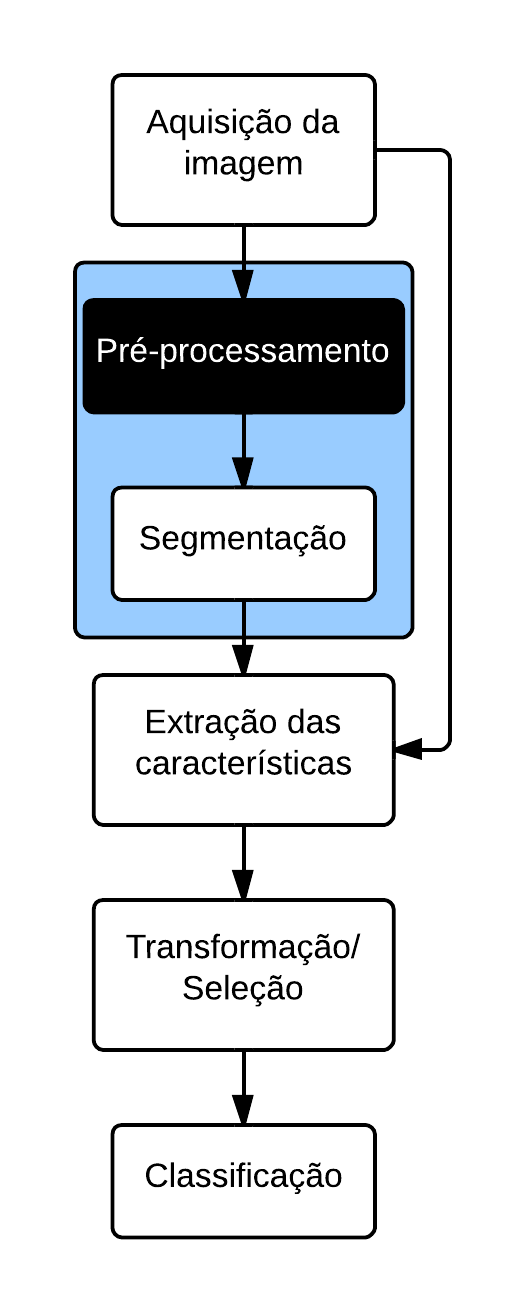
\includegraphics[width=0.3\linewidth]{figuras/flow.png}
 \end{center}
 \caption[Etapas canônicas do reconhecimento de padrões desde a aquisição da imagem até sua posterior classificação.]{Etapas canônicas do reconhecimento de padrões desde a aquisição da imagem até sua posterior classificação. As etapas de pré-processamento e segmentação --- apresentadas em destaque --- são normalmente pouco exploradas, quando comparadas com as etapas posteriores. O enfoque desse estudo é dar maior atenção à etapa de pré-processamento. \textit{Fonte:~Elaborado pela autora.}}
 \label{fig:etapascanonicas}
\end{figure}

\enlargethispage{-\baselineskip}

% Algumas pesquisas sobre os efeitos da sobreamostragem e geração de exemplos artificiais em dados de aprendizado de máquina já foram realizadas~\cite{Kuncheva2004,Chawla2002}. O método mais divulgado na literatura é conhecido como SMOTE (\textit{Synthetic Minority Over-sampling Technique}). Este método propõe a geração de exemplos artificiais a partir dos vetores de características originais das classes minoritárias. Não há registro conhecido de um estudo dessas técnicas em dados de informação visual para o rebalanceamento de classes.

Ao invés de focar em métodos complexos de transformação do espaço de características, propõe-se a redução da complexidade do problema no início do processo do reconhecimento, ao quantizar as imagens antes da extração de características. Embora a quantização normalmente faça parte do \textit{pipeline}, faltam estudos na literatura que descrevam o método de quantização e seus parâmetros. Ao negligenciar essa etapa, perde-se a oportunidade de redução da dimensionalidade e/ou do tempo de execução. Dessa forma, essa pesquisa propõe o utilização de menos de oito bits para armazenar as informações de cor (imagens quantizadas) e posteriormente extrair as características com dimensionalidade reduzida.

O desbalanceamento de classes também se apresenta como um obstáculo para que a classificação de imagens seja satisfatória. Esse problema é caracterizado pela diferença entre o número de exemplos disponíveis para cada classe da base de imagens. Em bases médicas, por exemplo, a quantidade de imagens relacionadas com uma doença rara é menor do que as imagens de pacientes sem a doença. Nessas situações, em que as imagens representam eventos importantes porém menos frequentes, o sistema de classificação pode ter problemas para lidar com a classe minoritária. Muitos métodos de transformação do espaço de características e de classificação assumem que as classes da base estão balanceadas, o que nem sempre é verdade. Propõe-se, portanto, a geração de imagens artificiais a partir do processamento das imagens originais, com o objetivo de rebalancear a base de imagens e consequentemente o modelo criado para a classificação. Esse método é comparado com o \sigla{SMOTE}{\textit{Synthetic Minority Over-sampling Technique}}, técnica de sobreamostragem dos vetores de características ao interpolar os exemplos mais próximos.

De maneira sumária, \textbf{esta pesquisa busca melhorar a classificação de imagens, utilizando métodos de processamento de imagens com foco na quantização e no rebalanceamento de classes, ambos antes da extração de características.} Os resultados obtidos, posteriormente apresentados na Seção \ref{cap:resultados}, demonstram o potencial do processamento de imagens antes da extração de características. Além disso, é fornecido uma visualização do espaço de características após o rebalanceamento das classes, crucial para analisar se as novas características extraídas são relevantes, ou seja, se adicionaram informações que estavam latentes ao aprendizado. Os resultados também demonstram que a quantização das imagens permite ao mesmo tempo obter vetores de características mais compactos e com maior capacidade de discriminação entre classes.


%--------------------------------------------------------------------------------
\section{Contextualização}

O grupo de pesquisa em Visualização, Imagens e Computação Gráfica (VICG), do Instituto de Ciências Matemáticas e de Computação (ICMC), tem atuado nas áreas de apoio para a classificação de coleções de imagens. Os trabalhos do grupo estão relacionados à visualização de informação com projeções multidimensionais e árvores~\cite{Joia2011}, assim como à extração de características e classificação de coleções de imagens~\cite{Paiva2011}. No que tange o processamento de imagens digitais, \citeonline{Picon2011} e \citeonline{Ponti2013} focam no pré-processamento para obter melhores resultados de classificação.

Ainda, \citeonline{Paiva2011} mostraram que os espaços de características formados por cor e textura podem ser melhorados, porém há um limite até o qual as características podem ser transformadas, ou selecionadas, de forma a garantir a discriminação entre as classes. Tal projeto atua na investigação de métodos que permitam gerar espaços de características com maior discriminação entre as classes, facilitando a classificação.

Em outros dois trabalhos relacionados é possível ver a diferença da performance para problemas de classificação de imagens. No primeiro, os autores atingem acurácia acima de 98\% na classificação de frutas após investigar alterações nos parâmetros de aquisição, realizar pré-processamento e obter a segmentação \cite{Rocha2010}. No segundo, os autores indicam que o método utilizado para obter a imagem em escala de cinza (comumente utilizada por algoritmos de extração), pode impactar significativamente a classificação final de diversas bases de imagens~\cite{Kanan2012}.

\meutodo{adicionar alguma pesquisa mais recente aqui}
\meutodo{adicionar http://arxiv.org/pdf/1602.03264v1.pdf}

%--------------------------------------------------------------------------------
\section{Hipóteses}

Conforme anteriormente mencionado, muitos aspectos influenciam a performance da classificação de coleções de imagens. É comum encontrar bases cuja extração de características é considerada difícil, ou seja, nas quais algoritmos canônicos de extração não conseguem extrair características que diferenciem bem as classes, prejudicando sua posterior classificação. Nessa situação, normalmente tenta-se lidar com as particularidades das características extraídas através de transformações no espaço de atributos ou mesmo projetando classificadores mais elaborados. Acredita-se que, ao invés disso, é importante investigar métodos de processamento e preparação de imagens antes da extração das características.

O objetivo desta pesquisa é explorar as etapas de processamento de imagens com o intuito de melhorar a discriminação entre classes de uma coleção de imagens. \textbf{Utilizar um número reduzido de cores juntamente com um método de quantização apropriado antes da extração de características pode permitir ao mesmo tempo obter vetores de características mais compactos e com maior capacidade de discriminação entre classes.} Analisando para tal, como a extração de características e posterior redução de dimensionalidade são afetados por diferentes métodos de quantização. Melhorando, assim, a classificação e diminuindo a complexidade do sistema.

Além disso, o desbalanceamento de classes é um obstáculo para uma classificação satisfatória, e por isso também é estudado. A hipótese, nesse caso, é que \textbf{a geração de imagens artificiais como preparação para a extração de características pode melhorar a acurácia da classificação, quando comparada à geração de exemplos artificiais no espaço de atributos.} Ou seja, gerar novas imagens artificiais — que serão posteriormente reduzidas a atributos — pode apresentar melhores resultados para a classificação do que o \textit{bootstrap} de atributos artificiais. Esse método é comparado com o SMOTE, técnica de sobreamostragem dos vetores de características ao interpolar os exemplos mais próximos.

\section{Contribuições}

Dados tais aspectos, pode-se então diferenciar as contribuições desta pesquisa:

\begin{description}
\item[Contribuição Geral] \

Investigar os métodos de pré-processamento de imagens de forma a preparar uma coleção de imagens para a extração de características. Com isso, espera-se observar o efeito da quantização de imagens na classificação e do balanceamento do número de instâncias de diferentes classes.

\item[Contribuições Específicas] \

  \begin{itemize}

    \item Demonstrar que é possível obter vetores de características compactos e efetivos ao extrair características de imagens com reduzido níveis de intensidade a um custo computacional baixo. Reduzindo o tamanho do vetor de características de métodos de descrição de cor após a quantização e possibilidade de redução do tempo de processamento para os métodos de descrição de textura;

    \item Demonstrar que a geração de imagens artificiais utilizando métodos de processamento --- como borramento, mistura e combinação de imagens --- pode contribuir com o balanceamento entre classes (em se tratando de problemas de classes desbalanceadas). Melhorando, dessa forma, o \textit{f1-score} resultante de algoritmos de classificação, quando comparada à geração de exemplos artificiais no espaço de atributos (SMOTE) e à classificação da base original.

  \end{itemize}
\end{description}

%--------------------------------------------------------------------------------
\section{Estrutura do documento}

O conteúdo desta dissertação está estruturado como segue.

\begin{description}
\item [Capítulo~\ref{cap:revisao}:] são conceituados os principais fundamentos necessários para o desenvolvimento desta pesquisa: pré-processamento de imagens, extração de características, desbalanceamento de classes e redução de dimensionalidade.

\item [Capítulo~\ref{cap:quantization}:] a redução do número de intensidades de cor utilizando métodos de quantização antes da etapa de extração de características é descrita.

\item [Capítulo~\ref{cap:metodo}:] descreve-se os métodos de processamento utilizados para a geração artificial de imagens --- sobre as imagens originais --- com o objetivo de rebalancear classes.

\item [Capítulo~\ref{cap:resultados}:] os resultados obtidos com a quantização e a geração de imagens artificiais são apresentados e discutidos.

\item [Capítulo~\ref{cap:conclusoes}:] reflete sobre as contribuições deste trabalho e apresenta os trabalhos futuros.

\end{description}


\chapter{Fundamentos}
\label{cap:revisao}
\section{Considerações iniciais}

Neste capítulo são destacados os tópicos mais relevantes para a compreensão do estado da arte de processamento de imagens, com foco na preparação das imagens para a extração de características. O problema do desbalanceamento de classes e seu efeito na classificação satisfatória também são abordados, assim como a extração de características para compreender as propriedades extraídas das imagens. Alguns trabalhos relacionados são utilizados como exemplo, com o objetivo de elucidar tais tópicos.

Inicialmente, a Seção~\ref{sec:preprocessamento} apresenta alguns dos principais métodos utilizados para o pré-processamento de imagens (i.e.\ remoção de ruído, realce de imagens e convolução), relevantes para o desenvolvimento desta pesquisa. Tendo como proposta melhor compreender o que são as características latentes, a Seção~\ref{sec:latentes} exemplifica as operações de pré-processamento utilizadas para visualizar tais características em uma aplicação específica. A extração de características é brevemente definida na Seção~\ref{sec:extracao}. Por fim, o problema do desbalanceamento de classes é apresentado na Seção~\ref{cap:desbalanceamento}. Nessa seção, além de caracterizar o problema, são apresentadas duas vertentes para solucioná-lo: sobreamostragem e subamostragem. Esses conceitos são necessários para a compreensão do capítulo de proposta desta dissertação.

% A área de \textit{deep learning} é definida e as redes de convolução e máquinas de Boltzmann restritas são contextualizadas no âmbito desta pesquisa.
% A seção seguinte (\ref{sec:deeplearning}) destaca o uso de \textit{deep learning} para o aprendizado de características e a Seção~\ref{sec:rbm} aborda as máquinas de Boltzmann restritas como método para aprendizado da distribuição das imagens de entrada.

%--------------------------------------------------------------------------------
\section{Pré-processamento de imagens}
\label{sec:preprocessamento}

Uma imagem digital $I$ pode ser definida como uma função $f(x,y)$, onde $x$ e $y$ são as coordenadas cartesianas de um determinado ponto e $f$ a intensidade (brilho) da imagem naquele ponto. Essa imagem é composta por finitos elementos chamados de pixels que podem ser diretamente acessados através de sua posição $x$ e $y$. Digitalmente, uma imagem é representada por uma matriz de valores com $M$ linhas e $N$ colunas onde cada elemento representa a sua intensidade. Uma imagem colorida $I$ do sistema RGB possui três canais de cores representantes das cores vermelha, verde e azul. Cada elemento $I(x,y)$ corresponde a uma tripla $(r, g, b)$ de números, com $0 \leq r \leq 255$, $0 \leq g \leq 255$ e $0 \leq b \leq 255$, onde 0 é a intensidade de cor mais escura e 255 a mais clara. A combinação dessas intensidades resulta na cor do pixel \cite{Gonzalez2007}. A Figura \ref{fig:pixel} mostra uma visualização ampliada dos pixels de uma imagem digital.

\begin{figure}[htbp]
 \begin{center}
   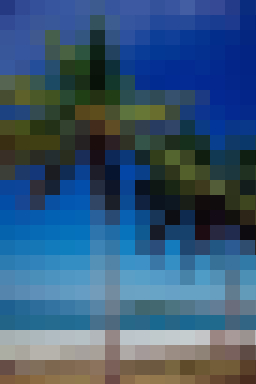
\includegraphics[width=0.4\linewidth]{figuras/pixel.jpg}
 \caption[Visualização pixelizada de uma imagem da base COREL-1000.]{Visualização pixelizada de uma imagem da base COREL-1000\footnotemark. \\ \textit{Fonte:~Elaborado pela autora.}}
 \label{fig:pixel}
 \end{center}
\end{figure}
\footnotetext{Disponível em http://wang.ist.psu.edu/docs/related/}
O processo de aquisição por um sistema de imageamento pode causar diversas imperfeições nas imagens, como pixels ruidosos, brilho inadequado e outras degradações. O pré-processamento de imagens é caracterizado por receber uma imagem de entrada e fornecer uma imagem de saída. Nessa etapa, efeitos indesejáveis podem ser eliminados e certas características realçadas (Figura \ref{fig:preproc}). Considera-se que um determinado critério utilizado para uma imagem pode não ser o mais eficiente para outra, dependendo assim da área de aplicação.

\vspace{12pt}
\begin{figure}[htbp]
 \begin{center}
   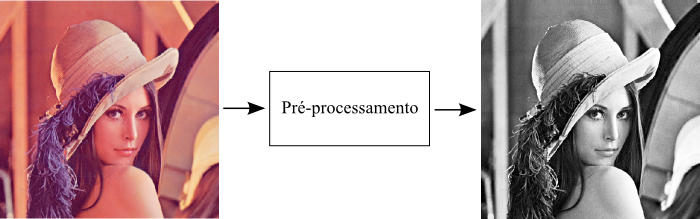
\includegraphics[width=1\linewidth]{figuras/preprocessamento.png}
 \caption[Sobre a imagem RGB de entrada foram realizadas operações de borramento, realce e de equalização de histograma. A imagem à direita é resultante dessas operações.]{O pré-processamento de imagens é caracterizado por receber uma imagem como entrada e fornecer uma imagem de saída. Sobre a imagem RGB de entrada (à esquerda) foram realizadas operações de borramento, realce e de equalização de histograma. A imagem à direita é resultante dessas operações. \textit{Fonte:~Elaborado pela autora.}}
 \label{fig:preproc}
 \end{center}
\end{figure}

% Alguns exemplos de técnicas utilizadas para o pré-processamento de dados para algoritmos de Aprendizado de Máquina são: amostragem, tratamentos para dados desbalanceados, limpeza dos dados, transformações e redução de dimensionalidade \cite{Faceli2011}.

Assim, técnicas de pré-processamento tornam os dados mais adequados para posterior análise, ao eliminar ou reduzir problemas como ruídos e imperfeições. Em \citeonline{Ponti2010}, o autor relata que a utilização de métodos de restauração na etapa de pré-processamento da imagem, antes da segmentação, resultou em uma qualidade superior para todos os testes, com valores de erro e desvio padrão menores. No referido estudo, métodos de realce causaram perda de informação e por isso não são indicados para uso em imagens obtidas por microscópio. O método indicado para evitar a amplificação de ruído nessas imagens é o algoritmo iterativo Richardson-Lucy, que será apresentado na Seção \ref{sub:deconvolucao}.

Em contrapartida, \citeonline{6} propuseram uma representação para imagens faciais baseada em características de textura, sem utilizar pré-processamento. Este aparece somente como sugestão de trabalho futuro, como possível correção de problemas do sistema de captura (i.e. suavização causada pela captura fora de foco). O que implica que, apesar dos bons resultados, a melhoria com a utilização de pré-processamento não foi investigada. Pode-se imaginar, portanto, que o uso de pré-processamento pode melhorar os resultados já obtidos, através do realce de textura e eliminação de imperfeições nas imagens.

Como exemplo do uso de métodos de pré-processamento, considere imagens de algas verdes obtidas por um microscópio de alta resolução. Essas algas são mergulhadas em um líquido que normalmente causa problemas de ruído e pouco contraste. Para a preparação dessas imagens, antes da extração de características, \citeonline{Borges2013} cita algumas etapas comuns em processamento de imagens digitais:

\begin{itemize}
\item As imagens -- originalmente em RGB -- são convertidas para uma escala de cinza;
\item A dimensão da imagem é reduzida para diminuir o tempo de execução dos passos subsequentes de processamento;
\item O constraste é ``ajustado'', para aumentar a diferença das intensidades dos pixels da imagem e corrigir o brilho;
\item A imagem é filtrada, removendo ruídos causados pelo processo de captura;
\item O contorno é realçado, pois a forma é uma das características mais importantes para discriminar algas (e outros objetos);
\item Por fim, o histograma é equalizado.
\end{itemize}

%--------------------------------------------------------------------------------
\subsection{Filtragem espacial e convolução}

% %--------------------------------------------------------------------------------
% \subsection{Convolução}
\label{sec:convolucao}

Um filtro espacial, também conhecido como \textit{kernel}, máscara ou janela, consiste em uma matriz de vizinhanças e uma operação a ser realizada nos pixels de uma imagem. A filtragem cria um novo pixel com as mesmas coordenadas do centro da vizinhança, contendo o valor resultante da filtragem. Dessa forma, a imagem filtrada contém os pixels resultantes da passagem do centro do filtro espacial por todos os pixels da imagem original \cite{Gonzalez2007}.

O processo de percorrer a imagem com um filtro espacial é chamado de correlação. A convolução, que pode ser definida como o operador $*$ na Equação \eqref{eq:conv}, é o mesmo processo, mas com o filtro previamente rotacionado em $180^{\circ}$ \cite{Gonzalez2007}.

\begin{equation}
\text{Mapa de características} = \text{imagem de entrada} * \text{filtro}
\label{eq:conv}
\end{equation}
% \vspace{0.2pt}

Os métodos de filtragem possuem como objetivo aperfeiçoar certos aspectos da imagem de entrada. Essa filtragem pode ser realizada no domínio da frequência ou no domínio espacial. Um filtro de suavização típico no domínio espacial é o de Gaussiana, que resulta no borramento e redução de ruído, a fim de remover detalhes da imagem (Figura~\ref{fig:blur}). Esse filtro utiliza uma função Gaussiana para calcular a transformação a ser realizada a cada pixel. A equação que representa a função Gaussiana em duas dimensões é definida por
\begin{equation*}
    G_{\sigma}(x,y) = \frac{1}{2\pi \sigma^2} e^{-\frac{x^2 + y^2}{2 \sigma^2}},
\label{eq:Gaussian}
\end{equation*}

\noindent onde $x,y$ são coordenadas de um determinado pixel da imagem e $\sigma$ o desvio padrão que determina o raio da distribuição Gaussiana aplicada. Valores altos de variância fazem com que o resultado da função se aproxime da média.

% A filtragem Gaussiana seletiva objetiva borrar áreas da imagem onde há pouco detalhe, porém preservando contraste e pequenas estruturas. Esse tipo de filtragem é dita adaptativa, pois modifica-se o parâmetro $\sigma$ (Equação~\ref{eq:Gaussian}) para cada pixel da imagem. Uma implementação dessa técnica utiliza a variância global da imagem $\sigma_g$ e variâncias locais $\sigma_r$, suavizando com maior intensidade regiões onde a $\sigma_r \leq \sigma_g$, e suavizando menos as regiões onde $\sigma_r > \sigma_g$.
\vspace{12pt}
\begin{figure}[!hbpt]
 \begin{center}
\begin{subfigure}{.4\textwidth}
  \centering
  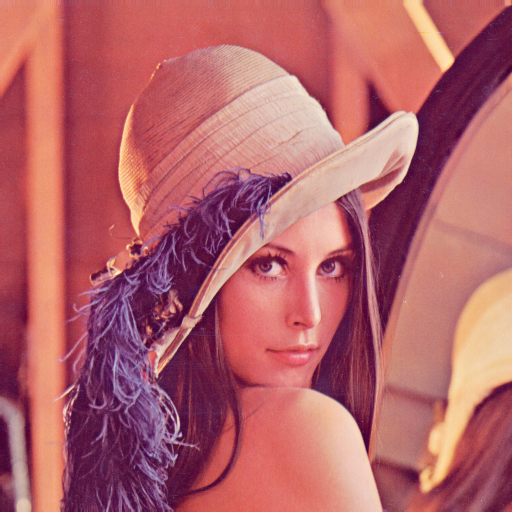
\includegraphics[width=\linewidth]{\detokenize{figuras/original.png}}
  \caption{Original}
\end{subfigure}
\hspace{0.1\textwidth}
\begin{subfigure}{.4\textwidth}
  \centering
  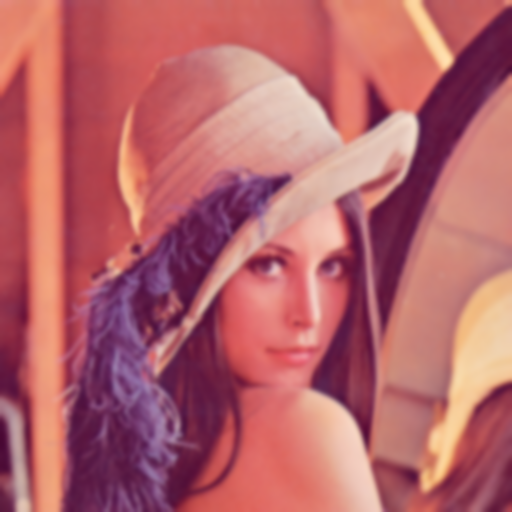
\includegraphics[width=\linewidth]{\detokenize{figuras/blur.png}}
  \caption{Filtrada}
\end{subfigure}
 \end{center}
 \caption[Exemplo de filtragem gaussiana como operação de pré-processamento.]{Exemplo de filtragem gaussiana como operação de pré-processamento. \textit{Fonte:~Elaborado pela autora.}}
 \label{fig:blur}
\end{figure}

%--------------------------------------------------------------------------------
\subsection{Deconvolução}
\label{sub:deconvolucao}

O processo de convolução, descrito na seção anterior, também pode ser definido como a passagem de uma imagem por um processo de aquisição que atue como um filtro de passa-baixas, resultando em uma imagem borrada. A deconvolução realiza a inversão desse borramento, o que pode facilitar a segmentação e detecção de características~\cite{Ponti2010}. Para tal, é necessário conhecer previamente ou estimar a função que causou a degradação na imagem, geralmente denotada por $h(\mathbf{u})$, onde $\mathbf{u}$ representa as coordenadas $(x,y,z)$ para um sinal tridimensional.

Em casos mais simples é possível utilizar o filtro pseudo-inverso, obtendo o filtro a partir da transformada de Fourier da função $h$, denotada por $H$ em
\begin{equation*}
W(\mathbf{u}) = \left\lbrace
      \begin{array}{ll}
    H(\mathbf{u}),  & H(\mathbf{u}) > \gamma \\
    \gamma,     & \text{ caso contrário},
      \end{array}
\right.
\end{equation*}
\noindent onde o limiar $\gamma$ utilizado é em geral um valor entre $0,0001$ e $0,1$. O filtro $W$ é utilizado para realizar a inversão, no domínio da frequências, da imagem $g$ borrada, obtendo a imagem restaurada a partir de

\begin{equation*}
    \hat{F}(\mathbf{u}) = \frac{G(\mathbf{u})}{W(\mathbf{u})},
\end{equation*}
\noindent onde $\hat{F}$ é a transformada de Fourier da imagem restaurada, $G$ é a transformada de Fourier da imagem borrada, e $W$ é o filtro pseudo-inverso, que realiza a deconvolução.

Um outro exemplo de algoritmo de deconvolução é o Richardson-Lucy~\cite{Ponti-Jr2011}, que utiliza um processo iterativo para recuperar uma imagem degradada que foi borrada por algum processo conhecido. Utiliza uma metodologia probabilística, baseada em EM-ML (\textit{Expectation-Maximization Maximum Likelihood}), para encontrar uma imagem que maximize a probabilidade de se visualizar a imagem original sem degradação, considerando um modelo de ruído de Poisson. O algoritmo é descrito na Equação~\ref{eq:RL}, onde $n$ é o número da iteração.

\begin{equation}
  \hat{f}_{n+1}(\mathbf{u})=
      \left[\left(
              \frac{g(\mathbf{u})}{\hat{f}_n(\mathbf{u})*h(\mathbf{u})}\right)
           *h(\mathbf{u})\right]
      \times \hat{f}_{n}(\mathbf{u}).
  \label{eq:RL}
\end{equation}
\vspace{2pt}

Algoritmos iterativos como o Richardson-Lucy tem a vantagem de permitir soluções parciais, evitando amplificação de ruído.

%--------------------------------------------------------------------------------
\subsection{Realce de imagens}

O realce de imagens é o processo de modificar uma imagem para que se torne mais adequada para uma aplicação específica do que na sua forma original. É subjetivo, porque depende do sujeito que está analisando a imagem dissernir a qualidade desse realce \cite{Gonzalez2007}.

Na Figura \ref{fig:pre-sharp} está demonstrado o efeito do algoritmo de \textit{unsharp masking}, utilizando como borramento um filtro de média. Com o objetivo de realçar imagens, os passos deste método são:

\begin{enumerate}
\item Borramento da imagem original;
\item Cálculo da diferença entre a imagem suavizada e a original;
\item Soma dessa diferença à imagem original.
\end{enumerate}

\begin{figure}[!htbp]
 \begin{center}
\begin{subfigure}{.4\textwidth}
  \centering
  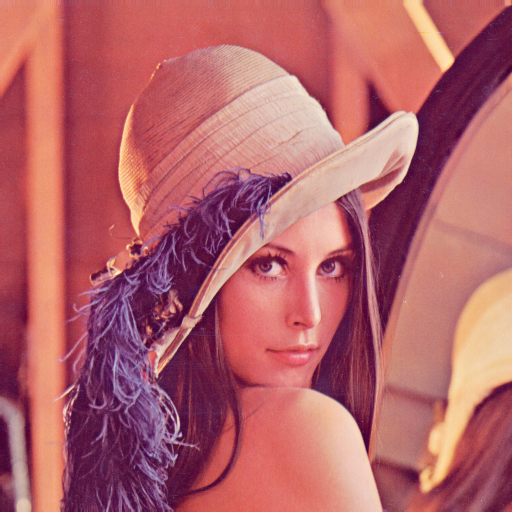
\includegraphics[width=\linewidth]{\detokenize{figuras/original.png}}
  \caption{Original}
\end{subfigure}
\hspace{0.1\textwidth}
\begin{subfigure}{.4\textwidth}
  \centering
  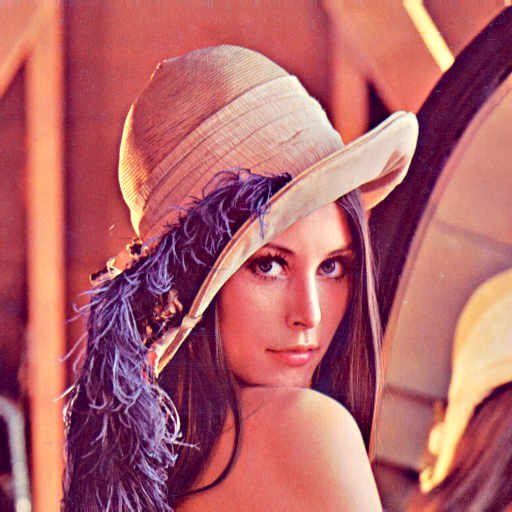
\includegraphics[width=\linewidth]{\detokenize{figuras/unsharpmask.png}}
  \caption{\textit{Unsharp masking}}
  \label{fig:unsharp}
\end{subfigure}
 \end{center}
 \caption[A imagem original, já em escala de cinza, foi realçada utilizando o método \textit{unsharp masking}.]{A imagem original, já em escala de cinza, foi realçada utilizando o método \textit{unsharp masking}. \textit{Fonte:~Elaborado pela autora.}}
 \label{fig:pre-sharp}
\end{figure}

% Uma variação do \textit{Unsharp Mask} é uma versão adaptativa apresentada por \cite{Polesel2000}. Essa solução pretende reduzir a sensibilidade a ruido e também evitar a adição de artefatos, com o objetivo de enfatizar os detalhes que contém contraste médio e sem aplicar sharpening em áreas suaves. O resultado disso é uma imagem com maior dinâmica em áreas de detalhe e sem mudança em áreas uniformes. Para classificar uma dada região entre essas três classes (alto, médio e nenhum detalhe) foi calculado a variância local de um bloco 3x3 pixels. Esse algoritmo utiliza dois filtros direcionais com coeficientes atualizados por uma estratégia de adaptação de Gauss-Newton.

Um exemplo clássico de utilização de realce, é para compensar a variação de iluminação em diversas imagens. Em \citeonline{Gross2003}, os autores propuseram um algoritmo para o reconhecimento de faces invariante à iluminação. Eles ressaltam que, desconsiderando a variação da posição, a iluminação é o fator de maior impacto na aparência das faces. A luz varia durante o dia, entre um dia e outro e entre diferentes ambientes. Isso afeta o conjunto de imagens a ser analisado, que passa a conter imagens com diferentes constrastes, o que pode acentuar ou diminuir certas características faciais.

O constraste é a diferença de intensidade entre os níveis de maior e menor intensidade na imagem. Imagens com baixa resolução podem ser geradas a partir de uma iluminação pobre ou outros problemas com a captura. Dessa forma, o processo de ``esticar'' o contraste expande os níveis de intensidade da imagem \cite{Gonzalez2007}.

\meutodo{Explicar melhor histograma e k}

É possível aumentar o contraste de uma imagem ao manipular o seu histograma $h$, que pode ser definido como
\begin{equation*}
h(i_k) = n_k,
\end{equation*}
\noindent onde $n_k$ é o número de pixels de intensidade $i_k$. Ao observar os histogramas de diferentes imagens é possível notar que imagens com alto contraste possuem um histograma com níveis próximos a uma distribuição uniforme. Isso permite que certas operações, como a equalização de histograma, obtenham o melhor contraste de uma imagem. Essa operação é caracterizada pela máxima variância do histograma e pode ser definida como
\begin{equation}
s_k = T(i_k) = \frac{L-1}{MN} \sum_{j=0}^{k}n_j,
\end{equation}
\noindent onde $L$ é o número de intensidades e $MN$ as dimensões da imagem. A imagem de saída é obtida ao mapear cada pixel de intensidade $i_k$ em um nível $s_k$, com $i$ entre $[0,L-1]$, sendo $i = 0$ um pixel preto e $i = L-1$, branco \cite{Gonzalez2007}.

\enlargethispage{\baselineskip}
%--------------------------------------------------------------------------------
\subsection{Restauração}

Ao contrário do realce, a etapa da restauração é objetiva. Também procura melhorar os aspectos visuais de uma imagem, mas com base em modelos probabilísticos de degradação de imagens. Dessa forma, tendo-se um modelo de degradação, procura-se recuperar a imagem original \cite{Gonzalez2007}. Mas um problema comum em algoritmos de remoção de ruído é que alguns detalhes, como textura, irão sofrer alta suavização.

O objetivo dos algoritmos de remoção de ruído é recuperar a imagem original. Assim o modelo estatístico da imagem natural é crucial para a remoção de ruído. O tipo mais simples de ruído  é o aditivo, que pode ser caracterizado como
\begin{equation*}
p = p_0 + n,
\end{equation*}
\noindent onde $p_0$ é o valor real do pixel e $n$ é a perturbação de ruído naquele pixel.

% A maneira mais simples de modelar o efeito de ruído em uma imagem digital é adicionar um ruído branco gaussiano, com média zero e variância $\sigma^2$.

Um algoritmo alternativo para remoção de ruído é o de médias não locais. Isso porque pixels similares não necessariamente estão próximos em suas coordenadas cartesianas, assim, informações não locais podem ser utilizadas na redução de ruído. De acordo com \citeonline{Buades2005}, dada uma imagem ruidosa $v = {v(i) | i \in I}$, o valor estimado é calculado como uma média ponderada de todos os pixels em uma mesma imagem com
\begin{equation*}
v(i)= \sum_{j \in I} w(i, j)v(j),
\end{equation*}
\noindent onde os pesos $w(i, j)$ dependem da similaridade entre pixels.

%--------------------------------------------------------------------------------
\subsection{Quantização}
\label{sec:quantizacao}

A maioria dos métodos de extração de características utiliza imagens de entrada em escala de cinza. Isso ocorre porque a complexidade de lidar com um pixel representado em três dimensões é muito maior do que em apenas uma dimensão. Assim, os métodos de quantização visam, de alguma forma, reduzir os canais de cores (24 bits) em apenas um (8 bits). \citeonline{Kanan2012} demonstraram que os métodos para a quantização (conversão de uma imagem colorida para escala de cinza) influenciam a performance no reconhecimento de imagens. Eles também salientam que o método utilizado deveria estar claramente descrito nas publicações da área.

% Em um trabalho recente \cite{Ponti2016}, com participação da autora desta dissertação, quatro métodos de quantização foram investigados. Foi constatado que os melhores métodos de conversão para escala de cinza antes da utilização dos descritores de características a serem mencionados na Seção \ref{sec:extracao} são:

\begin{description}
\item [Intensidade:] método mais simples, consiste em computar a média entre os canais RGB da imagem a partir de
\begin{equation*}
	Q_{Intensidade} = \frac{1}{3}(R + G + B)
\end{equation*}
\noindent e então realizar a correção por \textit{gamma}.

\item [Bits mais significativos (MSB):] ao invés de realizar uma combinação linear dos canais de cores, ordena os bits dos canais coloridos em um único canal. Computa quantos bits de cada canal de cor contribuem para a imagem final e extrai os bits do código binário dos canais originais \cite{Ponti-Jr2013}.
\end{description}

\meutodo{Adicionar aqui os métodos de quantização utilizados no paper}

A Figura \ref{fig:quantizacao} apresenta a conversão na escala de cinza obtida com o uso destes métodos.

\begin{figure}
 \begin{center}
\begin{subfigure}{.3\textwidth}
  \centering
  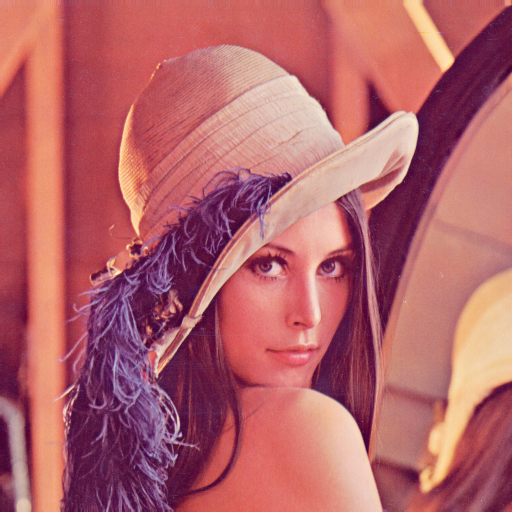
\includegraphics[width=\linewidth]{\detokenize{figuras/original.png}}
  \caption{Original}
\end{subfigure}
\begin{subfigure}{.3\textwidth}
  \centering
  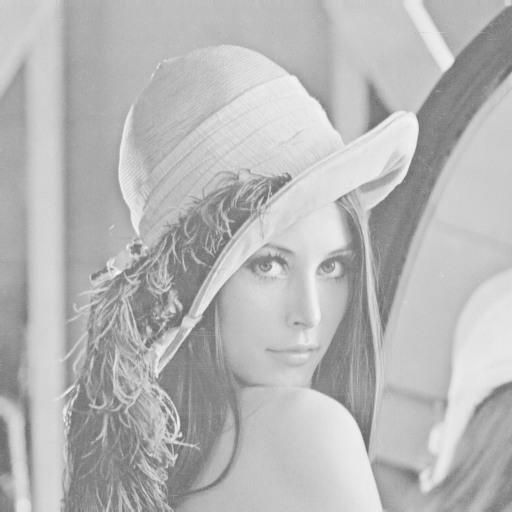
\includegraphics[width=\linewidth]{\detokenize{figuras/intensity.png}}
  \caption{Intensidade}
  \label{fig:intensidade}
\end{subfigure}
\begin{subfigure}{.3\textwidth}
  \centering
  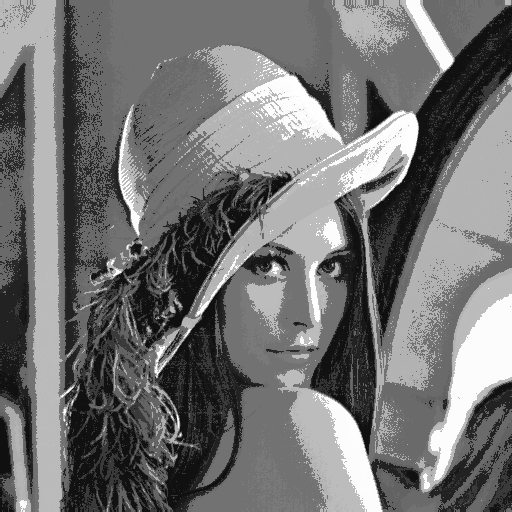
\includegraphics[width=\linewidth]{\detokenize{figuras/MSB.png}}
  \caption{MSB}
  \label{fig:msb}
\end{subfigure}
 \end{center}
 \caption[Conversão para a escala de cinza com os métodos de Intensidade e MSB.]{Conversão para a escala de cinza com os métodos de Intensidade e MSB. \textit{Fonte:~Elaborado pela autora.}}
 \label{fig:quantizacao}
\end{figure}

%--------------------------------------------------------------------------------
% \subsection{Reconstrução}

% \meutodo{Seção reconstrução? fisher faces}

% Fisherfaces é utilizado para reconhecimento de faces, reconstrói faces para a posterior classificação. No contexto deste estudo, esse método pode ser utilizado para gerar novas imagens a partir das já existentes como para auxiliar no problema do desbalanceamento de classes (descrito na Seção \ref{cap:desbalanceamento}). Especificamente para a sobreamostragem do conjunto de dados de entrada.

% Calcula os autovetores de todas as imagens de treinamento. Seleciona as com maior valor de autovalores.

% Primeiramente é realizado o cálculo do PCA para reduzir a dimensão $N-c$ (onde $N$ é o número de imagens e $c$ o número de classes) e então aplicado o FLD (\textit{Fisher Linear Discriminant}) para reduzir a $c-1$. A reconstrução tende a desconsiderar porções da imagem que não a discriminam. Considera cada pixel em uma imagem como uma coordenada.

% Esse método calcula a matriz de covariância das imagens originais e sua matriz de transformação $W$ com colunas ortonormais. Em seguida, tenta-se encontrar a melhor matriz $W$. Essa matriz é selecionada pela maximização da razão entre as matrizes de espalhamento intra e inter~\cite{Belhumeur1997}. Isso é expresso pela equação:

% \begin{equation}
% W = W_{FLD}^{T} W_{PCA}^{T}.
% \end{equation}

% As matrizes de transformação que projetam a matriz original é então dada por:

% \begin{eqnarray}
%     W_{PCA} &=& \operatorname{arg\,max}_{W} |W^T S_T W| \\
%     W_{FLD} &=& \operatorname{arg\,max}_{W} \frac{|W^T W_{PCA}^T S_{B} W_{PCA} W|}{|W^T W_{PCA}^T S_{W} W_{PCA} W|}
% \end{eqnarray}

% Essa matriz $W$ é portanto a reconstrução da imagem original.

%--------------------------------------------------------------------------------
\section{Extração de características}
\label{sec:extracao}

O objetivo da extração de características é descrever as informações visuais relevantes em um vetor de características. Esse vetor pode ser utilizado como entrada para um algoritmo de classificação de padrões. Como por exemplo, em aplicações que envolvem a classificação de algas, uma informação muito importante para a discriminação entre classes é a forma \cite{Borges2013}. Essas características devem salientar as diferenças entre imagens de classes distintas e suavizar possíveis diferenças de imagens da mesma classe. Algumas características, segundo~\citeonline{Gonzalez2007}, são:

\begin{description}
\item [Textura:] na sua descrição estatística, possui propriedades como: suavidade, aspereza e uniformidade. Um exemplo de medida para descrever a textura é a entropia.
\item [Forma:] representa os objetos em termos de suas características externas, como, por exemplo, a medida da curvatura.
\item [Cor:] considera a distribuição espacial de cores na imagem. O histograma de uma imagem pode descrever essa configuração de forma global.
\end{description}

Exemplos de métodos conhecidos capazes de descrever forma e outras características são: histogramas de orientação de gradiente~\cite{Wang2009}, curvatura, descritores de Fourier, métodos baseados na detecção de SUSAN~\cite{Smith1997}, Harris-Affine~\cite{Han2005b} e diferença de Gaussianas~\cite{Lowe2004a}. Os descritores utilizados no desenvolvimento desta pesquisa para a obtenção dos resultados da Seção~\ref{cap:resultados} estão abaixo descritos.

\begin{description}
\item[Histograma global de cor (GCH):] calcula o histograma global dos níveis de intensidade da imagem. É a alternativa mais simples para representar as informações de uma imagem~\cite{Gonzalez2007}. Produz um vetor de $N$ dimensões, sendo $N$ o número de intensidades.

\item[Vetor de coerência de cor (CCV):] captura informações sobre como as cores são organizadas em regiões conectadas, de acordo com um \textit{threshold}. Classifica os pixels da imagem em coerentes e incoerentes, computa os respectivos histogramas e os concatena \cite{ccv}. Dessa forma, o vetor de características produzido possui $2N$ dimensões.
% , uma dimensão para o número de pixeis coerentes e outra para incoerentes, que são determinados de acordo com um determinado threshold.

\item[Classificação de pixels de borda e interior (BIC):] computa dois histogramas, um para pixels definidos como borda e outro como interior. Se um pixel possuir a mesma cor que seus vizinhos, é pixel de interior; caso contrário, será pixel de borda. Os histogramas são concatenados, gerando um vetor de $2N$ dimensões \cite{bic}.

\item[Auto-correlograma de cor (ACC):] captura a correlação espacial entre cores idênticas. Computa a probabilidade de encontrar dois pixels com a mesma cor, a uma distância $d$ um do outro \cite{acc}. Neste estudo, são consideradas quatro distâncias: 1, 3, 5 e 7; resultando em um vetor com $4N$ características.

\item[Haralick-6:] extrai seis características a partir uma matriz de coocorrência: entropia, homogeneidade, contraste, correlação, probabilidade máxima e uniformidade. O vetor resultante possui 6 dimensões \cite{Haralick1973}.
\end{description}

%--------------------------------------------------------------------------------
\section{Características latentes}
\label{sec:latentes}

Assim como o método de quantização se mostrou relevante na classificação, nesta dissertação são estudados diversos métodos de pré-processamento de imagens, como filtros de borramento e deconvolução, com o objetivo de obter imagens processadas que sejam mais bem caracterizadas para a etapa de classificação (ou seja, aumentando a variância entre as classes, sem aumentar a variância intra-classe). O enfoque está em como realçar determinadas características, como por exemplo cor, textura e forma. A esses atributos pode-se dar o nome de características latentes, não visíveis na imagem original. Identificar e realçar tais características é objetivo deste estudo. Essa abordagem se diferencia das técnicas multi-resolução, pois não pretende encontrar apenas características em versões de diferentes resoluções (convoluídas com filtros passa-baixa), e sim também em versões deconvoluídas ou transformadas por outros operadores.

Se uma das principais características que diferenciam classes de uma certa base utiliza a sua forma, é possível utilizar o método de diferença de Gaussianas para ressaltá-la.
% Considerando, por exemplo, uma série de imagens filtradas por um filtro Gaussiano definido como $f_1(x,y) = G_{\sigma}(f(x,y))$.
O método DoG (\textit{Difference of Gaussians}) se baseia na diferença entre duas imagens filtradas. A operação comumente é feita usando $\sigma = \sqrt{2}$ e sua definição para dois níveis de filtragem é definida por
\begin{eqnarray*}
         f_1(x,y) &=& G_{\sigma}(f(x,y)) \\
         f_2(x,y) &=& G_{\sigma}(f_1(x,y)) \\
         DoG_1(x,y,\sigma) &=& f_2 - f_1
\end{eqnarray*}

A Figura~\ref{fig:caracteristicas} demonstra uma possível execução de filtragem e restauração seguida pela detecção de bordas por DoG, aplicadas em uma base de imagens de algas verdes.

\renewcommand{\tabcolsep}{0.0cm}
\begin{figure}[htbp]
 \begin{center}
\begin{subfigure}{.2\textwidth}
  \centering
  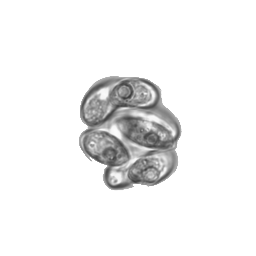
\includegraphics[width=\linewidth]{\detokenize{figuras/alga_05b.png}}
  \caption{}
  \label{fig:algaa}
\end{subfigure}
\begin{subfigure}{.2\textwidth}
  \centering
  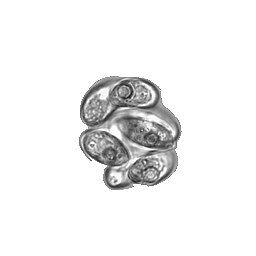
\includegraphics[width=\linewidth]{\detokenize{figuras/alga_05c.png}}
  \caption{}
  \label{fig:algab}
\end{subfigure}
\begin{subfigure}{.2\textwidth}
  \centering
    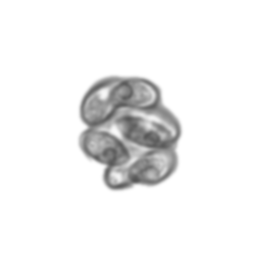
\includegraphics[width=\linewidth]{\detokenize{figuras/alga_05d.png}}
  \caption{}
  \label{fig:algac}
\end{subfigure}
\begin{subfigure}{.2\textwidth}
  \centering
  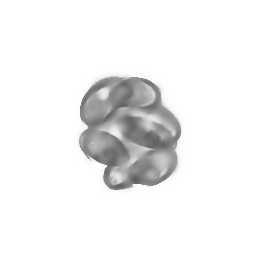
\includegraphics[width=\linewidth]{\detokenize{figuras/alga_05e.png}}
  \caption{}
  \label{fig:algad}
\end{subfigure}
\begin{subfigure}{.2\textwidth}
  \centering
  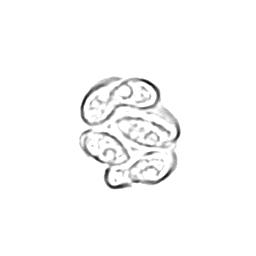
\includegraphics[width=\linewidth]{\detokenize{figuras/alga_05ba.png}}
  \caption{}
  \label{fig:algae}
\end{subfigure}
\begin{subfigure}{.2\textwidth}
  \centering
  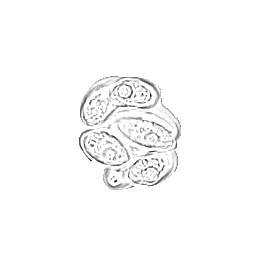
\includegraphics[width=\linewidth]{\detokenize{figuras/alga_05ca.png}}
  \caption{}
  \label{fig:algaf}
\end{subfigure}
\begin{subfigure}{.2\textwidth}
  \centering
  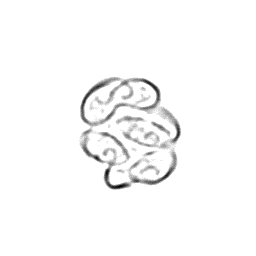
\includegraphics[width=\linewidth]{\detokenize{figuras/alga_05da.png}}
  \caption{}
  \label{fig:algag}
\end{subfigure}
\begin{subfigure}{.2\textwidth}
  \centering
  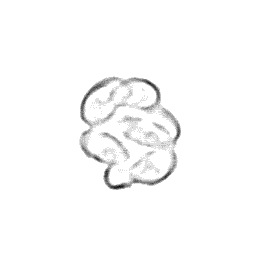
\includegraphics[width=\linewidth]{\detokenize{figuras/alga_05ea.png}}
  \caption{}
  \label{fig:algah}
\end{subfigure}
\begin{subfigure}{.2\textwidth}
  \centering
  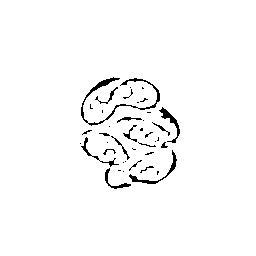
\includegraphics[width=\linewidth]{\detokenize{figuras/alga_05bb.png}}
  \caption{}
  \label{fig:algai}
\end{subfigure}
\begin{subfigure}{.2\textwidth}
  \centering
  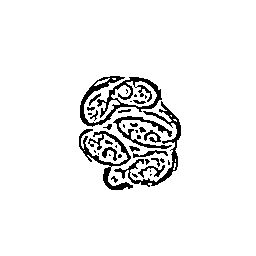
\includegraphics[width=\linewidth]{\detokenize{figuras/alga_05cb.png}}
  \caption{}
  \label{fig:algaj}
\end{subfigure}
\begin{subfigure}{.2\textwidth}
  \centering
  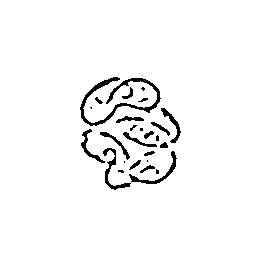
\includegraphics[width=\linewidth]{\detokenize{figuras/alga_05db.png}}
  \caption{}
  \label{fig:algak}
\end{subfigure}
\begin{subfigure}{.2\textwidth}
  \centering
  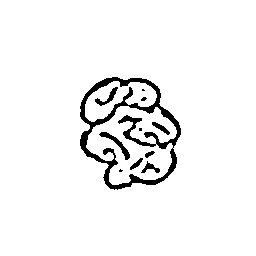
\includegraphics[width=\linewidth]{\detokenize{figuras/alga_05eb.png}}
  \caption{}
  \label{fig:algal}
\end{subfigure}

 \caption[Características latentes de algas verdes.]{Características latentes de algas verdes. A primeira imagem (a) é uma imagem original segmentada de alga. As próximas colunas são imagens resultantes da deconvolução da imagem (coluna 2), filtragem Gaussiana (coluna 3) e filtragem Gaussiana seletiva (coluna 4). A primeira linha mostra versões diferentes de imagens de algas, a segunda linha exibe imagens resultantes da diferença de Gaussianas, e a terceira linha demonstra imagens binárias obtidas por limiarização das imagens contidas na segunda linha). \textit{Fonte:~Elaborado pela autora.}}
 \label{fig:caracteristicas}
 \end{center}
\end{figure}
\renewcommand{\tabcolsep}{0.25cm}

A imagem \ref{fig:algaa} é uma imagem original segmentada de alga. As próximas colunas são imagens resultantes da deconvolução da imagem (coluna 2), filtragem Gaussiana (coluna 3) e filtragem Gaussiana seletiva (coluna 4). As modificações apresentadas na primeira linha geram informações em diferentes planos axiais da imagem de microscopia. Imagens na segunda coluna representam uma versão deconvoluída das imagens originais, ressaltando a textura na superfície das algas, resultantes da diferença de Gaussianas. Já a terceira linha demonstra imagens binárias obtidas por limiarização das imagens da segunda linha, realçando as características da base da célula.

Acredita-se que ao manipular as imagens através de técnicas de pré-processamento, pode-se gerar imagens artificiais com características latentes realçadas, melhorando a extração de características.

%--------------------------------------------------------------------------------
% \section{Deep learning}
% \label{sec:deeplearning}
%
% % O cérebro humano está em constante aprendizado. Suponha que uma determinada pessoa nunca tenha visto um \textit{drone}. Ela então lê uma pesquisa recente sobre esses veículos aéreos contendo uma foto de um exemplar. Enquanto isso, essa tecnologia acaba se tornando mais acessível e surgem várias publicações na mídia sobre eles. Após tê-los visto algumas vezes, essa pessoa será capaz de reconhecer visualmente um \textit{drone} em imagens, vídeos e até mesmo de diferentes cores e tamanhos em relação às imagens que tinha visto anteriormente.
%
% % Dessa forma, ao se expor a alguns padrões, ela aprendeu a reconhecê-los. Essa capacidade dos sistemas de aprendizado (como o cérebro humano) de reconhecer novos padrões está diretamente relacionada com a capacidade de generalização. Nesse sentido, generalizar é como ter visto um \textit{drone} de cor preta medindo 1 metro e ao ver um outro de cor branca de 20 metros, classificá-lo como sendo um \textit{drone} também, porque aprendeu as principais características.
%
% A habilidade humana de reconhecimento de padrões em imagens é surpreendente. Os algoritmos de aprendizado de máquina e de reconhecimento de padrões tentam habilitar os computadores a aprender, baseando-se no modelo de aprendizado de seres humanos \cite{thesisDeep}. Considerando que existem milhões de neurônios em cada córtex visual e que o cérebro humano é composto por cinco desses córtex que evoluíram durante milhões de anos, pode-se afirmar que a tarefa de algoritmos de reconhecimento de padrões em imagens não é simples \cite{neuralNielsen}.
%
% A capacidade humana de reconhecer novos padrões está diretamente relacionada com a capacidade de generalização, que para tal, utiliza hierarquias \cite{thesisDeep}. Nessa linha, o aprendizado profundo ou \textit{deep learning} é caracterizado por explorar o aprendizado ao simular o funcionamento do cérebro humano. Essa área está diretamente relacionada com aprendizado de máquina e inteligência artificial e lida com o aprendizado através de múltiplas camadas.
%
% Explicitar quais são as regras para aprender um determinado conceito pode se tornar impossível. No caso de um avião, por exemplo, ``voar'' pode ser uma regra decomposta em ``possuir largura maior que altura'' e ``ser aerodinâmico''. Essas subdivisões geram múltiplos níveis que possuem maior complexidade e abstração, de maneira similar ao aprendizado por camadas. Uma rede neural artificial utiliza imagens como treinamento para automaticamente inferir quais são as regras para o reconhecimento. São chamadas de redes neurais profundas ou \textit{deep neural networks} as redes que possuem uma estrutura de muitas camadas -- duas ou mais ocultas \cite{neuralNielsen}. Assim, dada uma imagem como entrada, o problema é subdividido em problemas mais simples de serem resolvidos, podendo chegar ao nível de pixels isolados.
%
% As redes neurais artificiais consistem em um método para solucionar problemas de forma a simular o comportamento do cérebro humano. Ao tentar uma determinada solução e errar, essas redes aprendem e podem tentar novamente. Ou seja, adquirem conhecimento através da experiência. Elas contém neurônios de entrada, ocultos e de saída. Aprender nesse contexto significa encontrar os pesos que fazem com que a rede neural exiba o comportamento esperado \cite{Schmidhuber2014}.
%
% % Hubel e Wiesel publicaram em 1962 uma pesquisa relacionada ao estudo do córtex visual primário de gatos. Eles identificaram células simples, similares aos layers de bancos de filtros de uma ConvNet e células complexas similares aos layers de pooling.
%
% A simulação desse modelo inspirado biologicamente utilizada hoje é de \citeonline{lecun1998} e chama-se Rede Neural de Convolução (CNN ou ConvNet). Eles simplificaram tal arquitetura para utilizar um algoritmo de retropropagação para o treino. Desde então, essas redes vêm sendo utilizadas para detecção, reconhecimento, restauração, remoção de ruído e segmentação de imagens e vídeos, além de sua aplicação em áudio. Um exemplo de utilização dessa rede inspirada no modelo de LeCun foi desenvolvida pela empresa Google, com o objetivo de detectar faces e placas de carros para proteger a privacidade nas imagens de StreetView \cite{google09}.
%
% % \meutodo{Figura da visualização do resultado dos filtros}
%
% Apesar de redes profundas representarem o estado da arte em visão computacional, um bom entendimento das suas propriedades ainda está faltando. Alguns artigos recentes como \citeonline{Mahendran2014}, \citeonline{Zeiler2011} \citeonline{Zeiler2013} e \citeonline{Simonyan2013} introduzem técnicas utilizadas para analisar o comportamento e operações internas dessas redes ao visualizá-las. Esta pesquisa situa-se nesse viés, ao analisar as características latentes extraídas por uma rede neural de convolução.
%
% Para o uso em bases desbalanceadas, as imagens utilizadas para o rebalanceamento de forma visual podem ser geradas após o estudo das características latentes, encontradas no treinamento da classe minoritária em uma CNN. Essas características também podem ser realçadas de forma a melhorar a classificação de imagens.
%
% %--------------------------------------------------------------------------------
% \subsection{Redes de convolução}
% % As redes de convolução são modelos que podem aprender características, e são compostas por diversas camadas.
%
% São um tipo de rede neural que utiliza uma operação chamada de convolução, previamente descrita na Seção \ref{sec:convolucao}. Pode ser entendida como sendo várias multiplições de um filtro espacial pela imagem de entrada, resultando em um mapa de características ativadas. Esse filtro é um vetor de parâmetros capaz de aprender. Cada imagem possui seu conjunto de mapas de características, mas os filtros são comuns a todas as imagens. Dependendo dos valores do filtro, as características ativadas são diferentes. Nesse contexto, a camada de convolução consiste em muitas aplicações de convolução em paralelo, dado que um filtro é capaz de extrair apenas um tipo de característica \cite{Bengio-et-al-2014-Book}.
%
% Basicamente, uma CNN é uma arquitetura que pode aprender características invariantes. Com múltiplas camadas, ela pode aprender multiníveis de características \cite{lecun2010}. Ou seja, permite ao computador criar conceitos complexos a partir de conceitos simples. Como o conceito de \textit{deep learning} enfatiza o uso de variáveis latentes, sugere que algoritmo de treinamento pode inventar os conceitos que precisa para representar determinada base de dados \cite{Bengio-et-al-2014-Book}.
%
% Cada camada é composta de três estágios~\citeonline{lecun2010}, representados na Figura~\ref{fig:cnn}:
%
% \begin{description}
% \item [Estágio de convolução:] várias convoluções em paralelo para produzir um conjunto de ativações pré-sinápticas;
% \item [Estágio de detecção:] função de ativação, como a unidade linear retificada ou a sigmoide;
% \item [Estágio de \textit{pooling}:] retorna uma representação invariante a pequenas translações da entrada. Um exemplo é utilizar o valor máximo entre vizinhos (conhecido como \textit{max-pooling}). %Essa operação é de pós-processamento.
% \end{description}
% \begin{figure}[htbp]
%  \begin{center}
%    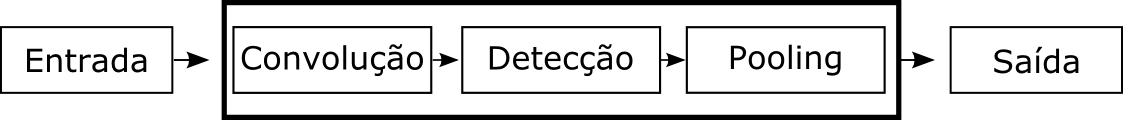
\includegraphics[width=1\linewidth]{figuras/convlayer.png}
%  \end{center}
%  \caption[Componentes típicos de uma camada de uma rede neural de convolução.]{Componentes típicos de uma camada de uma rede neural de convolução. Nessa terminologia a rede possui camadas complexas que possuem estágios \cite{Bengio-et-al-2014-Book}. \textit{Fonte:~Elaborado pela autora.}}
%  \label{fig:cnn}
% \end{figure}
%
% % Normalmente o kernel é muito menor que a imagem, o que resulta em menos parâmetros a serem armazenados, o que reduz o uso de memória e melhorando a eficiência.
% % Cada membro do kernel é usado em todas as posições da entrada, provocando invariância a translação. Por isso só é interessante usar uma camada de convolução quando o que é para ser aprendido é invariante a translação. Em alguns casos, como detecção de faces, não é tão interessante -- deve procurar a sombrancelha em cima e o queixo embaixo.
% % Ao processar dados temporais, o resultado de séries de convoluções produzem uma espécie de timeline ou mapa que mostra quando e aonde características diferentes aparecem na entrada.
% % Não é invariante a escala e a rotação.
% % É possível aprender invariâncias utilizando pool sobre as saídas das convoluções. Essa etapa sumiariza as respostas sobre uma vizinhança inteira, assim é possível utiilizar menos unidades de pooling do que unidades de detecção, resultando em um downsampling.
% % Uma característica essencial na implementação é o método escolhido para adição de zeros nas bordas da imagem. Sem isso o tamanho da representação diminui a kernel-1 a cada camada.
% % % Se pensarmos na convolução como uma multiplicação por uma matriz esparsa que possui cada elemento do kernel copiado várias vezes, a multiplicação da imagem de entrada pela transposta dessa matriz permite backpropagar os erros.
% % Para termos aprendizagem, é preciso computar o gradiente a respeito do kernal, dado o gradiente das saídas.
%
% De acordo com \citeonline{Bengio-et-al-2014-Book}, durante a propagação são realizadas as convoluções e propagadas pelo resto da rede para então computar uma função de perda, que mede quão bem o sistema de aprendizado funcionou para cada exemplo. Na retropropagação, recebe-se um gradiente para atualizar os pesos. O gradiente descendente estocástico atualiza o sistema de aprendizagem com base no erro medido para um único exemplo. Apesar de a convergência ser mais ruidosa do que calcular a média sobre todos os erros, diminui-se um custo constante do calculo de custo.
%
% Normalmente, o classificador é a última camada totalmente conectada, que computa o produto de um vetor de características \cite{Bengio-et-al-2014-Book}. \citeonline{Mahendran2014} reportam que as camadas inteiramente conectadas podem ser invertidas a uma imagem resultante da composição de partes similares às encontradas na imagem original, mas não idênticas. Enfatizam também que todas as camadas de convolução mantém uma representação fiel da imagem. Essa característica permite a análise de quais atributos são relevantes para o aprendizado da base de imagens, tarefa crucial para esta pesquisa.
%
%
% % % --------------------------------------------------------------------------------
% % \subsection{Redes de deconvolução}
%
% \citeonline{Zeiler2011} propuseram uma rede de deconvolução para a visualização das camadas, que pode ser vista como o caminho inverso de uma rede de convolução. Dessa forma, ao invés de mapear pixels em características, faz-se o contrário, permitindo a construção não supervisionada de representação de imagens hierárquicas, que podem, por exemplo, ser usadas para redução de ruído \cite{Zeiler2013}. Tenta gerar o sinal de entrada dada a soma das convoluções dos mapas de características com os filtros aprendidos. Apesar de destacar que, dado o mapa de características latentes, é possível sintetizar uma imagem, o artigo de \citeonline{Zeiler2011} não discorre sobre essa síntese.
%
%
% % Em \citeonline{Zeiler2013}, eles reverteram as computações para identificar quais pedaços das imagens eram responsáveis por certas ativações neurais. Olham sobre como certos outputs são obtidos
% % Mas nesse artigo: http://arxiv.org/pdf/1412.0035v1.pdf eles reconstroem as imagens. Dessa forma, eles mostram que as CNN retêm inforações fotograficamente precisas sobre a imagem, com diferentes graus de invariância.
% % Qual informação é preservada pela saída da rede.
% % A representação aprendida pode então ser utilizada para síntese. Em \cite{Zeiler?} um exemplo de redução de ruído é apresentado. Ao utilizar as características latentes da segunda camada para reconstruir a imagem, o ruído foi reduzido de 13.84dB para 18.01dB.
%
% % A operação de reconstrução pode ser definida como:
%
% % % \begin{equation}
% % % Ŷ_1 = (F_1)(U_(s_1))...(F_L)(U_(s_L)) = (R_l)(z_L)
% % % \end{equation}
%
% % % Com $ŷ_1$ sendo a imagem reconstruída, F a convolução, U unpool, z o mapa de características, s os switches de pooling e L o número de camadas.
%
% %--------------------------------------------------------------------------------
% \section{Máquinas de Boltzmann restritas}
% \label{sec:rbm}
%
% Uma máquina de Boltzmann restrita (RBM) é uma rede neural estocástica que treina um modelo a partir dos vetores de entrada. Ela aprende os parâmetros que definem a distribuição sobre um conjunto de observações sem retropropagação e baseando-se em energia \cite{Fischer2014}.
%
% Diferente de uma rede de Hopfield, ela agrega probabilidades e encontra a mínima energia global. Faz isso através do arrefecimento simulado (\textit{simulated annealing}), ou seja: em um primeiro momento, quando possui energia alta, aceita configurações piores; e conforme a energia é reduzida, detêm-se a uma região e a explora melhor, até o equilíbrio térmico \cite{Hinton2006}.
%
% Possuindo uma arquitetura muito mais simples que a CNN, é composta por duas camadas de neurônios: uma visível e outra oculta. Os pixels correspondem às unidades visíveis e os detectores de características às unidades ocultas. A sua restritividade se deve ao fato da falta de conectividade entre os neurônios de uma mesma camada, mas cada unidade visível é conectada a todas as unidades ocultas. Assim, a camada oculta, de detectores de características, modela a correlação entre os pixels.
%
% A aprendizagem de uma RBM começa em um estado aleatório e atualiza seus pesos até encontrar uma distribuição que esteja em equilíbrio. Essa convergência ocorre quando o erro entre os exemplos treinados -- fase positiva -- e suas reconstruções -- fase negativa -- é menor que um certo limiar. Dessa forma, a cada iteração, um novo exemplo é treinado ao repetir iterativamente esses dois estágios e atualizar seus pesos \cite{Hinton2006}.
%
% \begin{description}
% \item [Fase positiva:] fixa a camada visível e computa o valor dos neurônios ocultos. A probabilidade de um neurônio oculto ser ativado (se torne igual a 1) é dada pela função
% \begin{equation}
% p(h_j = 1) = \frac{1}{1+e^{-(b_j+\sum_{i\epsilon vis}{v_iw_{ij}})}},
% \label{eq:prob}
% \end{equation}
% \noindent onde $p(h_{j})$ é a probabilidade do neurônio $h_j$ ser ativado, utilizando uma função de ativação sigmóide, e $w_{ij}$ o peso entre a entrada $i$ e o neurônio $j$.
%
% A contribuição da fase positiva é computada para cada par de unidades $a_{ij}$, ao conferir se os dois neurônios ($x_i$ e $x_j$) estão ativados por meio de
% \begin{equation*}
% Fase_{+}(a_{ij}) = x_i . x_j
% \end{equation*}
%
% \item [Fase negativa:] a partir dos valores computados na fase positiva, os neurônios visíveis são ``reconstruídos'' ($p(v_i)$) e os ocultos novamente computados ($p(h_{j'})$) a partir da função de probabilidade da Equação \eqref{eq:prob}.
%
% % \begin{equation}
% % p(h_i = 1) = \frac{1}{1+e^{-(b_i+\sum_{j\epsilon vis}{v_jw_{ji}})}}
% % \label{eq:phi}
% % \end{equation}
%
% A contribuição da fase negativa é calculada da mesma forma que a contribuição positiva, com
% \begin{equation*}
% Fase_{-}(a_{ij}) = x_i . x_j
% \end{equation*}
%
% \item [Atualização dos pesos:] os pesos $w_{ij}$ são ajustados considerando a diferença entre os neurônios visíveis reconstruídos e os valores fornecidos de entrada inicialmente (etapa conhecida como \textit{contrastive divergence}):
% \begin{equation*}
% w_{ij} = w_{ij} + L (Fase_{+}(a_{ij}) - Fase_{-}(a_{ij})),
% \end{equation*}
% \noindent onde $L$ é a taxa de aprendizado. Quanto menor esse valor, melhor o treinamento e maior tempo até a convergência.
% \end{description}
%
%
%
% % Hinton e Seynowsky, em 1983, estenderam o modelo de Hopfield com a incorporação de dinâmica estocástica. Este modelo de rede neural passou a ser conhecido como Máquina de Boltzmann.
%
% % \begin{equation}
% % E(v,h) = - \sum{iEvisivel}{a_i v_i} - \sum{jEoculta}{b_j h_j} - \sum{i, j}{v_i h_j W_ijs}
% % \end{equation}
%
% % onde $v_i$ é o estado binário da unidade visível, $h_j$ estado binário da unidade oculta, $a_i$ e $b_j$ seus biases e $w_ij$ o peso entre eles.
% Essas redes também podem ser usadas como classificadores, ao treiná-las para modelar a relação entre a distribuição de entrada e seus respectivos rótulos \cite{Fischer2014}. Devido à capacidade das máquinas de Boltzmann restritas de aprender representações das imagens, pode-se utilizá-las para identificar se uma imagem é relevante para o aprendizado. Pode-se, por exemplo, utilizar apenas um neurônio, com a matriz de pesos representando uma memória associativa, para entender quais imagens são mais relevantes dentro de uma classe arbitrária. Dessa forma, também é possível avaliar a relevância da informação contida em uma imagem artificialmente gerada.

%--------------------------------------------------------------------------------
\section{Desbalanceamento de classes}
\label{cap:desbalanceamento}

Nesta seção é definido o problema do desbalanceamento de classes e apresentados os trabalhos relacionados que possuem duas diferentes abordagens: sobreamostragem (\textit{over-sampling}) e subamostragem (\textit{under-sampling}).

Em conjuntos de dados desbalanceados, determinadas classes possuem um número muito maior de instâncias do que outras. As classes com mais elementos são chamadas de classes majoritárias, e as com menos elementos, de minoritárias. O desempenho de algoritmos de Aprendizado de Máquina é prejudicado quando tratam de bases de dados desbalanceados. Esses algoritmos tendem a favorecer a classificação de um novo objeto à classe majoritária, pois esta fica muito melhor representada após o treinamento do que a minoritária. Considera-se, então, que esse problema é um obstáculo para a classificação satisfatória. Porém, como apontado por \cite{Batista2004}, o desbalanceamento não é o único responsável por reduzir o desempenho de algoritmos de aprendizagem. Eles sugerem que é possível haver uma ótima classificação mesmo contendo alto desbalanceamento na base de dados. Assim, a motivação do estudo de vários algoritmos para rebalanceamento não é apenas balancear os dados de treinamento, mas obter uma melhor diferenciação entre as classes. Isso porque o desbalanceamento por si só não é um problema, mas em conjunto com a sobreposição de classes pode diminuir significativamente a acurácia da classificação da classe minoritária. Os resultados reportados também mostram que a poda de árvores de decisão raramente levou a alguma melhora na classificação.

\cite{Castro2011} destacam que duas abordagens têm sido utilizadas para solucionar esse problema: pré-processar os dados de forma a rebalancear as distribuições das classes ao reamostrar os dados; ou então modificar métodos de aprendizado -- como através da adição de melhores funções de custo na classificação. Em geral, são reportados melhores resultados obtidos por algoritmos de \textit{over-sampling}, os quais consistem em reamostrar os dados aumentando o número de elementos da classe minoritária \cite{Batista2004}. Esta pesquisa tem como enfoque o \textbf{pré-processamento dos dados}, ao rebalancear as classes através da \textbf{geração de imagens artificiais}.

\subsection{Sobreamostragem}
\label{sec:smote}

Realizar uma sobreamostragem (\textit{over-sampling}) em um determinado conjunto de dados significa aumentar -- utilizando alguma estratégia -- o número de elementos desse conjunto. Em \cite{Chawla2002}, a simples replicação de exemplos pertencentes à classe minoritária não melhorou a classificação. Isso se deve ao reconhecimento de regiões muito específicas, causando \textit{overfitting}.

O SMOTE (\textit{Synthetic Minority Over-sampling Technique}) é um método desenvolvido por \cite{Chawla2002} para rebalancear classes ao gerar artificialmente novos elementos, ao invés de apenas replicá-los. É aplicado sobre os vetores de características previamente extraídos, com operações de perturbação dos dados de treino no espaço de características, e não no espaço dos dados. A diferença entre o vetor de características de um elemento e do seu vizinho mais próximo é multiplicada por um número $0 \le  x \le 1$. Esse valor é adicionado ao vetor original, criando um novo elemento. Como pode ser visualizado na Figura~\ref{fig:smote}, essa abordagem provoca a geração de um elemento resultante da interpolação dos dois vetores originais. Os exemplos sintéticos forçam uma região de decisão maior e mais geral para serem aprendidas como exemplos da classe minoritária.

% \begin{figure}[thpb]
% \centering
% 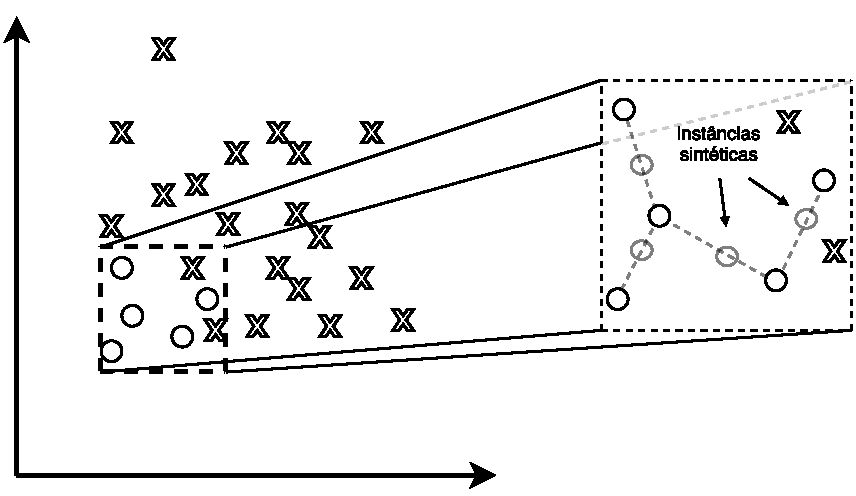
\includegraphics[width=0.7\linewidth]{figuras/smote}
% \caption{SMOTE: interpolação entre dois exemplos vizinhos no espaço de características.} %
% \label{fig:smote}
% \end{figure}

\meutodo{fazer a imagem do smote}

\begin{algorithm}[H]
  \caption{Algoritmo do SMOTE}
  \label{alg:smote}
  \SetAlgoLined
  \Entrada{Imagem colorida $I$ em formato BGR}
  \Saida{Exemplos sintéticos}
  $N \gets \text{vizinhos(minoritária)}$\;
  \ParaCada{exemplo $sample$}{
    $nn \gets \text{vizinho aleatório de N}$
    \ParaCada{\text{característica} $(x,y)$}{
      $\text{diferença} \gets nn(x,y) - sample(x,y)$\;
      $\text{gap} \gets \text{número aleatório entre 0 e 1}$\;
      $\text{G}(x,y) \gets sample(x,y) + gap*\text{diferença}$\;
    }
    $S \gets S U G$\;
  }
\end{algorithm}

Dessa forma, o SMOTE provê mais elementos para o classificador aprender, ao contrário da replicação de dados. Como trabalhos futuros, os autores \citeonline{Chawla2002} apontam que diferentes estratégias para criar esses exemplos sintéticos podem melhorar a performance da classificação. Inclusive salientando exemplos que foram errôneamente classificados.

Uma variação desse algoritmo, denominada Borderline-SMOTE1 \cite{Han2005}, considera que elementos fora da linha de borda de cada classe pouco contribuem para a classificação. Por isso, propôe a geração de elementos sintéticos utilizando apenas elementos de borda. Considera que se os vizinhos mais próximos são da classe majoritária, o exemplo é ruído, e se há mais vizinhos da classe majoritária do que da minoritária, considera esse elemento como sendo de borda. Como trabalho futuro, destacam a necessidade de considerar diferentes estratégias para definir em quais elementos realizar o over-sampling.


\subsection{Subamostragem}

Ao contrário da sobreamostragem, a subamostragem visa diminuir o número de elementos de um determinado conjunto. A ideia é eliminar elementos da classe majoritária que estão distantes da fronteira de decisão, isso porque eles são considerados menos relevantes para a aprendizagem.

Métodos para remoção de exemplos da classe majoritária normalmente apresentam resultados piores do que métodos de sobreamostragem, conforme relatado por \citeonline{Batista2004} e \cite{Japkowicz2002}. Um dos motivos pela preferência natural à sobreamostragem é o fato de que ao realizar subamostragem pode-se remover informações essenciais dos dados originais. Mas não há uma estratégia única que funcione melhor para todos os cenários.

%-------------------------------------------------------------------------------
\section{Classificadores de padrões}
\label{cap:classificadores}

% \subsection{Naive Bayes}

% Os métodos probabilísticos bayesianos definem que a probabilidade de classificar um objeto como sendo de uma classe não depende apenas da relação entre eles, mas também  de observar a independência entre eles \cite{Faceli2011}. O teorema de Bayes é utilizado para calcular a probabilidade de um objeto $B$ pertencer a uma classe $A$:

% \begin{equation}
% P(A|B) = P(B|A)P(A)/P(B)
% \end{equation}

% \noindent onde $P(A|B)$ é a probabilidade de um exemplo $B$ pertencer à classe $A$; $P(A)$ a probabilidade ``a priori'' da classe e $P(B)$ que pode ser estimado pela frequência com que um novo exemplo ocorre, que pode ser ignorado por ser o mesmo para todas as classes \cite{Faceli2011}.

\subsection{Algoritmo k-Vizinhos Mais Próximos}

K-NN é um classificador supervisionado que considera a proximidade entre os dados para realizar predições. Baseia-se na premissa de que os objetos do mesmo conceito são semelhantes. Na fase de treinamento, apenas armazena os exemplos rotulados do conjunto de dados de treinamento. Quando um novo exemplo deve ser classificado, calcula a distância entre os vetores de características do novo exemplo e aqueles já rotulados. O novo exemplo é então classificado como sendo da classe do exemplo de treinamento com menor distância~\cite{Boiman2008}.

\begin{enumerate}
\item Escolhe o valor de $k$ e uma métrica de distância;
\item Encontra os $k$ vizinhos mais próximos do exemplo que queremos classificar;
\item Rotula o sample como pertencente à classe que recebeu mais votos.
\end{enumerate}

\meutodo{figura aqui}

Esse classificador foi utilizado por ser suscetível à diferenciação entre as classes. Com $K = 1$, a predição da classe corresponde ao exemplo mais próximo.
%-------------------------------------------------------------------------------
\section{Redução de dimensionalidade}
\label{sec:vis}
% http://ieeexplore.ieee.org/stamp/stamp.jsp?tp=&arnumber=4368165

A visualização do espaço de características obtido após a geração artificial de imagens pode ajudar a verificar se as novas imagens melhoram a definição da classe minoritária em relação ao espaço original (inclusive antes de imagens serem removidas para provocar o desbalanceamento). Ou seja, se o método utilizado revelou características latentes. Dessa forma, ao projetar os novos vetores no espaço das imagens originais, é possível analisar qual método (entre SMOTE ou geração de imagens no campo visual) mais se assemelha à distribuição original dos dados.

Considerando que um vetor de características extraído com extratores comuns pode possuir entre 6 (e.g.\ Haralick) e 512 (e.g.\ BIC) características, a visualização de um exemplo requer que seja realizado o mapeamento desses valores em apenas duas dimensões. Para isso, uma redução de dimensionalidade mapeia os dados de $N$ dimensões para um espaço 1D, 2D ou 3D. A partir desses novos dados, pode então ser criada alguma representação visual que tente manter a relação de distância entre os novos e os originais~\cite{Paulovich2007}.

%%%%%%%%%%%%%%%%%%%%%%%%%%%%%%%%%%%%%%%%%%%%%%%%%%%%%%%%%%%%%%%%%%%%%%%%%%%%%%%%
\subsection{Análise de componentes principais}
\label{sec:pca}

% http://sebastianraschka.com/Articles/2014_pca_step_by_step.html
% http://arxiv.org/pdf/1404.1100v1.pdf

O PCA (Análise de Componentes Principais) é uma técnica não supervisionada que pode ser utilizada para reduzir a dimensionalidade dos dados com a máxima variância possível. Cada imagem, originalmente representada por um vetor com $N$ características, pode então ser representada por apenas um ou mais valores. Essa redução permite a projeção dessas imagens no espaço de características. O objetivo é extrair as informações mais importantes dos dados e representá-las como um conjunto de variáveis ortogonais chamadas de componentes principais. Para isso encontra-se uma outra base: uma combinação linear da base original, que melhor representa os dados ao assumir que as direções das maiores variâncias são as mais importantes. Ou seja, a variância associada com cada direção quantifica o quão principal é aquela direção \cite{Abdi2010}. Pode-se, portanto, enumerar os passos necessários para o PCA sendo:

\begin{enumerate}
\item Centraliza todos os atributos em zero ao subtrair a média de cada dimensão;
\item Calcula a matriz de covariância $C_x$ dada por
\begin{equation}
    C_x = X X^T,
\end{equation}

\noindent onde $X$ é a matriz de dados original e $X^T$ sua transposta;

\item Encontra os autovalores e autovetores de $C_x$. Um autovetor $u$ de uma matriz $A$ pode ser definido por $Au = \lambda u$, onde $\lambda$ é um autovalor escalar associado ao autovetor. Um vetor $u$ é um autovetor da matriz $A$ se o tamanho do vetor -- e não sua direção -- é modificado quando multiplicado por $A$. Os autovalores podem ser representados na diagonal de uma matriz $\lambda$ (com outros valores como zero) e o conjunto dos autovetores de $A$ em uma matriz $U$. Assim,

\begin{equation}
    A = U \lambda U^T;
\end{equation}

\item Então, os autovetores são ordenados de forma decrescente de acordo com seus autovalores correspondentes e escolhe-se os $k$ principais autovetores (i.e.\ maiores autovalores) para formar uma matriz $P$ de dimensão $n \times k$, onde cada coluna representa um autovetor. O valor $k$ será a quantidade de dimensões do novo espaço de atributos;
 % O novo espaço de atributos pode ser encontrado multiplicando a transposta dessa matriz pela transposta dos atributos originais. - caso seja svd
\item O novo subespaço pode ser encontrado multiplicando essa matriz $P$ pela matriz original, de acordo com a equação $Y = PX$, onde $X$ representa o conjunto de dados original, $Y$ é uma nova representação desses dados e $P$ a matriz ortonormal que transforma $X$ em $Y$. As linhas de $P$ são os componentes principais de $X$.
\end{enumerate}

%%%%%%%%%%%%%%%%%%%%%%%%%%%%%%%%%%%%%%%%%%%%%%%%%%%%%%%%%%%%%%%%%%%%%%%%%%%%%%%%
\subsection{\textit{Locality Preserving Projections}}
\label{sec:lpp}

LPP é um algoritmo linear de redução de dimensionalidade com propriedades de preservação da estrutura local dos dados. Não te a dificuldade dos algoritmos tradicionais (como PCA) de manter o manifold não linear dos dados originais \cite{Zhuo2014}. Embora o método mais utilizado para redução da dimensionalidade de forma não-supervisionada seja o PCA, métodos como esse produzem melhores projeções em termos de separação das classes. Em \cite{Zhuo2014} o LPP alcançou a melhor relação entre complexidade computacional e a redução da dimensionalidade, enquanto manteve a acurácia. Seu algoritmo segue três passos principais \cite{He2004}:

\begin{enumerate}
\item Constrói um grafo de adjacências. Os nós $i$ e $j$ possuem uma aresta entre eles se fazem parte do conjunto de $k$-vizinhos mais próximos de cada nó (sendo $k$ um parâmetro do algoritmo);

\item Encontra os pesos: $W_ij = 1$ se os vértices $i$ e $j$ estão pertos, ou seja, conectados por uma aresta e $W_ij = 0$ caso contrário;

\item Computa os autovalores e autovetores
\begin{equation}
    X L X^T a = \lambda X D X^T a,
\end{equation}
\noindent onde D é a matriz diagonal na qual a entrada são as somas das colunas de $W$
\end{enumerate}

A matriz de projeção corresponde aos autovetores, sendo os d menores autovalores.

%--------------------------------------------------------------------------------
\section{Considerações finais}

Deu-se destaque à discussão das etapas de pré-processamento e realce de características latentes, ambas foco deste estudo, assim como a geração de imagens artificiais para o balanceamento de classes. Este capítulo apresentou diversos métodos para exemplificação, além de trabalhos similares.

A extração de características foi abordada, apresentando os principais descritores utilizados nesta pesquisa. A lacuna destacada é que existem características não passíveis de extração por descritores convencionais.
% Para isso, as redes de convolução são apresentadas, pois possuem capacidade de aprender as características relevantes das imagens de entrada. Justificando, assim, seu uso para análise das propriedades das bases de imagens. Podem também indicar possíveis operações para auxiliar na geração de imagens artificiais. Ainda, a memória associativa aprendida por máquinas de Boltzmann restritas pode ser indicadora de quais imagens geradas adicionam informações ao aprendizado.
A geração dessas imagens visa rebalancear classes que diferem em número de imagens, e detalhes sobre esse problema também foram fundamentados nesse capítulo.

Esses fundamentos permitem compreender em que contexto esta dissertação de mestrado está inserida. O próximo capítulo abrangerá a proposta deste trabalho.


\chapter{Quantização de Imagens}
\label{cap:quantization}
%%%%%%%%%%%%%%%%%%%%%%%%%%%%%%%%%%%%%%%%%%%%%%%%%%%%%%%%%%%%%%%%%%%%%%%%%%%%%%%%
\section{Considerações iniciais}

Sistemas de reconhecimento de imagens comumente utilizam uma imagem em níveis de cinza 8-bits com 256 intensidades para a extração de características. Ao aplicar a quantização (redução de cores) na etapa de pré-processamento, é esperada a redução da complexidade do vetor de características logo no início, beneficiando todos os passos subsequentes.

Para analisar o impacto da utilização da quantização, são utilizados diferentes parâmetros de quantização combinados com quatro métodos de extração de cor e um de textura. Esses extratores foram escolhidos de acordo com os resultados apresentados por \citeonline{Penatti2012}.

Este capítulo trata dessa ideia de quantizar as imagens antes da extração de características, ligando com os métodos apresentados nos fundamentos.

%%%%%%%%%%%%%%%%%%%%%%%%%%%%%%%%%%%%%%%%%%%%%%%%%%%%%%%%%%%%%%%%%%%%%%%%%%%%%%%%
\section{Quantização de imagens}

O pipeline de reconhecimento de imagens envolve um passo de converter imagens coloridas em imagens com apenas um canal, obtendo uma imagem quantizada que pode ser então processada por métodos de extração de características. Dessa forma, cada imagem -- originalmente no espaço de cor RGB -- é convertida a um único canal com $C$ níveis de intensidade. Após, são utilizados os métodos apresentados na Seção \ref{sec:extracao} para extrair as características.
A Figura \ref{fig:quant:flow} ilustra esses passos, da aquisição até a classificação das imagens.

\begin{figure}[htbp]
  \begin{center}
    \centering
    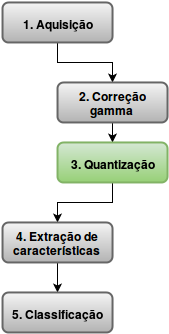
\includegraphics[width=0.25\linewidth]{\detokenize{figuras/quantizacao/quantizationFlow.png}}
  \end{center}
  \label{fig:quant:flow}
\end{figure}

Cada método de quantização se comporta diferentemente para uma dada imagem RGB. Por exemplo, o método Intensidade mapeia todas as permutações dos mesmos valores em RBG para a mesma cor. Assim, produz um plano no cubo RBG conforme mostrado na Figura \ref{fig:quant:plano}. O Gleam também é similar, mas spanning uma superfície curva, dada a natureza da função gamma. O mesmo efeito é alcançado utilizando Intensidade'. Em todos os casos, o resultado é o mapeamento de características cromáticas bem diferentes em valores de intensidades similares. O método Luminância tenta melhorar isso ao adicionar um peso na combinação linear dos canais.

\begin{figure}[htbp]
  \begin{center}
    \centering
    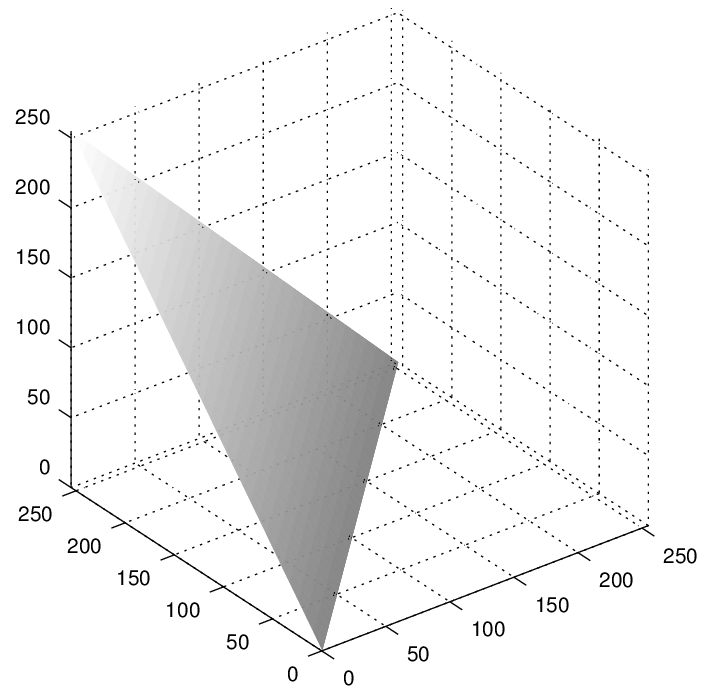
\includegraphics[width=0.5\linewidth]{\detokenize{figuras/quantizacao/plano.png}}
  \end{center}
  \caption[Plano computado pelo método de conversão para escala de cinza Intensidade, quando um dos canais de cor possui valor 255.]{Plano computado pelo método de conversão para escala de cinza Intensidade, quando um dos canais de cor possui valor 255. \textit{Fonte:~\cite{Ponti2016}.}}
  \label{fig:quant:plano}
\end{figure}

Um exemplo das imagens obtidas após os métodos de quantização apresentados anteriormente pode ser visto na Figura \ref{fig:quant:quantizacoes}. Nesse caso é possível notar que tanto Luminância quanto MSB conseguem melhor discriminar cores. Além disso, o mapa de cores MSB obteve um maior número de cores únicas. A barra de gradientes abaixo da imagem dos pinceis demonstra como os métodos de quantização se comportam dada a variação de cor.

\begin{figure}[htbp]
  \begin{center}
    \begin{subfigure}{.25\textwidth}
      \centering
      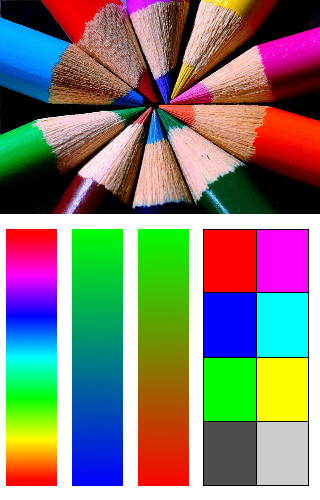
\includegraphics[width=\linewidth]{\detokenize{figuras/quantizacao/fig_quanttest.png}}
      \caption{Original}
      \label{fig:quant:original}
    \end{subfigure}
    \begin{subfigure}{.25\textwidth}
      \centering
      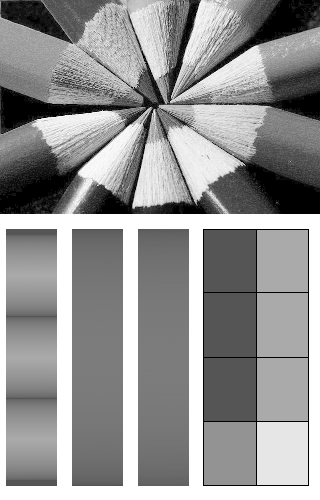
\includegraphics[width=\linewidth]{\detokenize{figuras/quantizacao/fig_quantGleam.png}}
      \caption{Gleam}
    \end{subfigure}
    \begin{subfigure}{.25\textwidth}
      \centering
      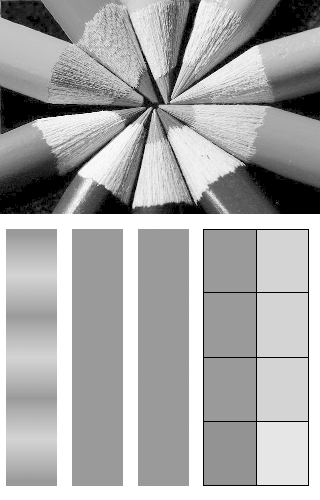
\includegraphics[width=\linewidth]{\detokenize{figuras/quantizacao/fig_quantIntensity.png}}
      \caption{Intensidade'}
    \end{subfigure}
    \begin{subfigure}{.25\textwidth}
      \centering
      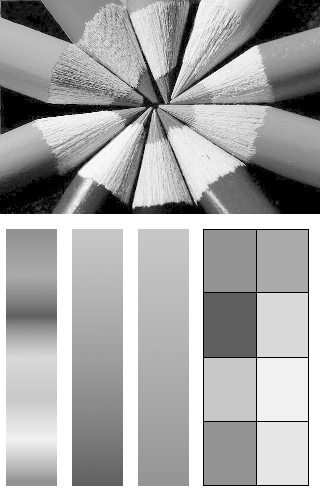
\includegraphics[width=\linewidth]{\detokenize{figuras/quantizacao/fig_quantLuminance.png}}
      \caption{Luminance'}
    \end{subfigure}
    \begin{subfigure}{.25\textwidth}
      \centering
      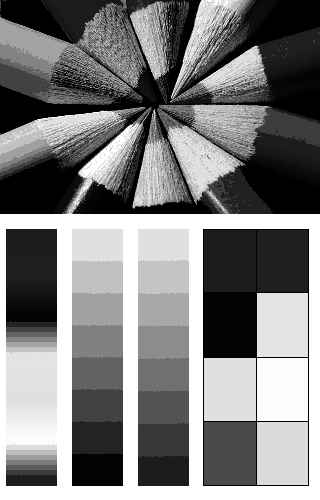
\includegraphics[width=\linewidth]{\detokenize{figuras/quantizacao/fig_quantMSB.png}}
      \caption{MSB}
    \end{subfigure}
    \hspace{0.1\textwidth}
  \end{center}
  \caption[Resultado da aplicação de métodos de quantização. A imagem original \protect\subref{fig:quant:original} resultou em versões de um canal de cor com 232 cores unicas para MSB e 184 cores para os restantes métodos.]{Resultado da aplicação de métodos de quantização. A imagem original \protect\subref{fig:quant:original} resultou em versões de um canal de cor com 232 cores unicas para MSB e 184 cores para os restantes métodos. \textit{Fonte:~\cite{Ponti2016}.}}
  \label{fig:quant:quantizacoes}
\end{figure}

% A Tabela \ref{tab:quantizacao} apresenta alguns exemplos numéricos, com a saída de cada método. Nesse caso, as entradas são tuplas de valores $(R, G, B)$. Note que a correção \textit{gamma} deve ser computada em um intervalo de valores reais $0-1$, que depois é mapeado para o intervalo $0-255$.

Na Figura \ref{fig:quant:avioes} é demonstrado um exemplo de redução de cores utilizando o método MSB para um par de imagens da base de dados Caltech-101. Importante destacar que há preservação das cores, especialmente entre 64 e 256. Ao utilizar apenas 32 cores, as imagens ainda são satisfatórias mas há uma perda de informação considerável.

\begin{figure}[htbp]
  \begin{center}
    \centering
    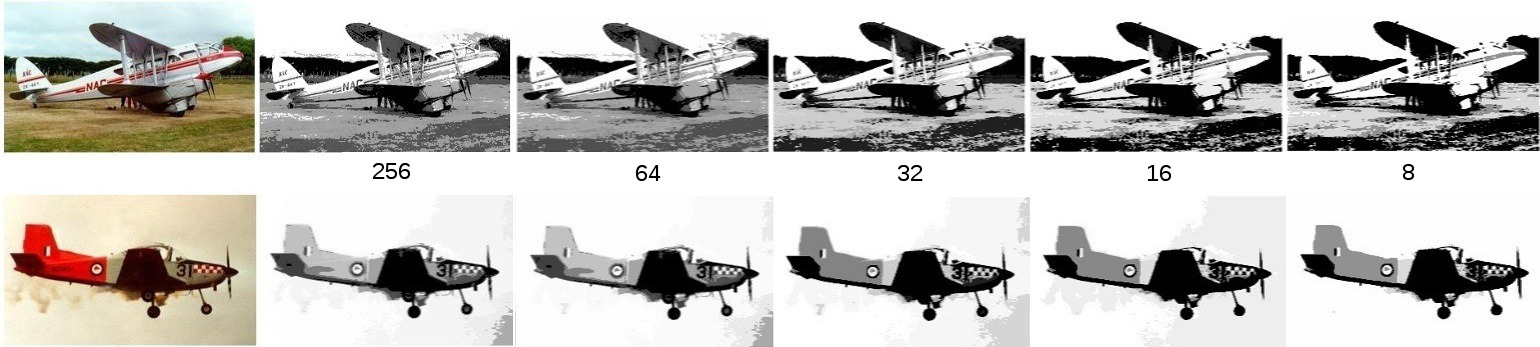
\includegraphics[width=\linewidth]{\detokenize{figuras/quantizacao/fig_quantizationexample.jpg}}
  \end{center}
  \caption[Duas imagens da base de dados Caltech101 com variações no parâmetro de cor utilizando o método MSB. Da esquerda para a direita: imagem original 24-bits e na sequência suas versões quantizadas com: 256, 64, 32, 16 e 8 cores.]{Duas imagens da base de dados Caltech101 com variações no parâmetro de cor utilizando o método MSB. Da esquerda para a direita: imagem original 24-bits e na sequência suas versões quantizadas com: 256, 64, 32, 16 e 8 cores. \textit{Fonte:~\cite{Ponti2016}.}}
  \label{fig:quant:avioes}
\end{figure}

%%%%%%%%%%%%%%%%%%%%%%%%%%%%%%%%%%%%%%%%%%%%%%%%%%%%%%%%%%%%%%%%%%%%%%%%%%%%%%%%
\section{Considerações finais}


\chapter{Geração Artificial de Imagens}
\label{cap:metodo}
\section{Considerações iniciais}


O processo de manipular imagens para que elas se tornem mais satisfatórias para um determinado objetivo depende do domínio de aplicação. Ou seja, não existe uma teoria geral para melhorar qualquer tipo de imagem \cite{Gonzalez2007}: um método que processa melhor uma imagem bem definida pelas suas cores difere do processamento de imagens texturizadas, às quais um processamento sobre a intensidade dos pixels da imagem -- como uma operação de borramento -- pode ocasionar perda da textura. Assim, justifica-se a exploração de um vasto número de métodos de processamento de imagens e bases.

Nesta pesquisa oito métodos de processamento de imagens são aplicados nas imagens minoritárias originais, gerando imagens artificiais. Isso é realizado a fim de permitir a extração de informações latentes com o objetivo de melhorar a classificação com alguma técnica de Aprendizado de Máquina, o que reflete a melhora da diferenciação entre as classes. Dada a quantidade de imagens necessárias para rebalancear a base original, são geradas imagens utilizando cada um dos métodos, além de uma versão combinando todos eles (ou seja, compondo um conjunto com algumas imagens processadas por cada método) e outra apenas replicando as imagens como \textit{baseline}. Como demonstrado na Figura~\ref{fig:escolha}, dado o conjunto de treinamento da classe (ou classes) com menor número total de imagens, é realizado o rebalanceamento ao aplicar os métodos descritos neste capítulo e posteriormente essas imagens resultantes são utilizadas como treinamento.

Neste capítulo os métodos de geração artificial para o rebalanceamento de classes de imagens são descritos. Os experimentos posteriormente destacados no Capítulo~\ref{cap:resultados} foram realizados utilizando: borramento; mistura ponderada; \textit{unsharp masking}; composição; combinação de thresholds; combinação com saliência; visual SMOTE; e adição de ruído.

\begin{figure}[htbp]
  \begin{center}
    \includegraphics[width=0.7\linewidth]{\detokenize {figuras/rebalance.pdf}}
  \end{center}
  \caption[Geração artificial a classe minoritária para rebalancear as classes.]{Geração artificial a classe minoritária para rebalancear as classes. \textit{Fonte: Elaborado pela autora.}}
  \label{fig:escolha}
\end{figure}

% Não foi testado uma porcentagem fixa para verificar se existe algum ganho em utilizar
% uma ponderação específica.

%  \begin{figure}[hbpt]
%  \begin{center}
%    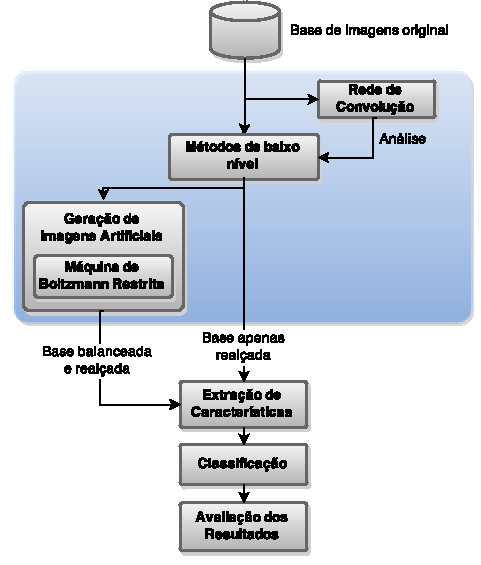
\includegraphics[width=1\linewidth]{\detokenize {figuras/geral.pdf}}
%  \end{center}
%   \caption[]{\textit{Fonte: Elaborado pela autora.}}
%  \label{fig:escolha}
% \end{figure}

%%%%%%%%%%%%%%%%%%%%%%%%%%%%%%%%%%%%%%%%%%%%%%%%%%%%%%%%%%%%%%%%%%%%%%%%%%%%%%%%
\section{Borramento}

Também conhecido como filtro de suavização, o borramento é uma operação de processamento comumente utilizada com o objetivo de filtrar as baixas frequências de uma imagem, removendo ruídos e detalhes não relevantes. Normalmente esse tipo de filtro provoca também um certo borramento das bordas, como pode ser observado na Figura~\ref{fig:blur}.

Esse comportamento não é esperado quando devemos gerar novas imagens, pois informações relevantes podem ser removidas. Dessa forma, a operação de borramento utilizada é a de filtro bilateral. Ela substitui o valor do pixel $(x,y)$ por uma média dos pixeis de intensidade similar na imagem e dos pixeis vizinhos \cite{Tomasi1998}. Ou seja, é uma média ponderada das intensidades. O Algoritmo~\ref{alg:blur} descreve os passos desse filtro e a Figura~\ref{fig:gen:blur} exemplifica o seu funcionamento: à esquerda está demonstrada a imagem original e à direita a imagem borrada.

\vspace{0.5cm}
\begin{algorithm}[H]
  \caption{Algoritmo de borramento com filtro bilateral}
  \label{alg:blur}
  \SetAlgoLined
  \Entrada{Imagem colorida $I$ em formato BGR}
  \Entrada{Diâmetro $d$ de pixinhança de pixels}
  \Entrada{Sigma do espaço de cor}
  \Entrada{Sigma do espaço de coordenadas}

  \Saida{Imagem gerada $G$}

  \meutodo{Algoritmo de filtro bilateral}
\end{algorithm}
\vspace{0.5cm}

\begin{figure}[htbp]
  \begin{center}
    \begin{subfigure}{.4\textwidth}
      \centering
      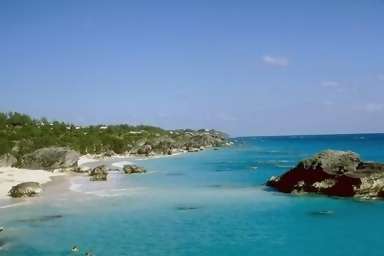
\includegraphics[width=\linewidth]{\detokenize{figuras/geracao/blur-a.png}}
      \caption{Original}
    \end{subfigure}
    \hspace{0.1\textwidth}
    \begin{subfigure}{.4\textwidth}
      \centering
      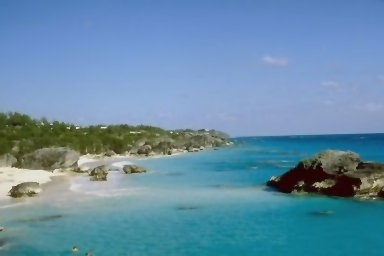
\includegraphics[width=\linewidth]{\detokenize{figuras/geracao/blur-b.png}}
      \caption{Imagem artificial}
    \end{subfigure}
  \end{center}
  \caption[Geração artificial utilizando borramento com filtro bilateral.]{Geração artificial utilizando borramento com filtro bilateral. \textit{Fonte:~Elaborado pela autora.}}
  \label{fig:gen:blur}
\end{figure}

\begin{description}
  \item[Parâmetros e suas variações] Conforme descrito no Algoritmo~\ref{alg:blur}, os parâmetros para essa geração são: o diâmetro $d$ de pixinhança de pixels, o $\sigma$ do espaço de cor e o $\sigma$ do espaço de coordenadas. Esses parâmetros dependem das propriedades das imagens e dos resultados pretendidos. Dessa forma, o tamanho do filtro é um valor escolhido arbitrariamente para cada aplicação em específico \cite{Tomasi1998}. Como o nosso objetivo com a geração das imagens não foi especializar no comportamento de uma classe de imagens específica, um valor foi escolhido aleatoriamente e a partir dele os parâmetros de entrada foram definidos.

  \item[Limitações] Esse filtro tende a remover texturas e a criar novos contornos. Dependendo dos valores, pode gerar uma imagem ``cartoonizada''.

  \item[Métodos relacionados] São diversos os métodos de borramento descritos na literatura, como a filtragem Gaussiana, a de mediana e a de médias.

  \item[Visualização] É interessante notar na Figura \ref{vis:blur} o comportamento da adição de imagens borradas para o rebalanceamento de classes bem descritas pela propriedade da cor.

  \meutodo{colocar aqui alguma figura do espaço... }

\end{description}
%%%%%%%%%%%%%%%%%%%%%%%%%%%%%%%%%%%%%%%%%%%%%%%%%%%%%%%%%%%%%%%%%%%%%%%%%%%%%%%%
\section{Aguçamento}

Diferentemente da suavização, o processamento de aguçamento procura enfatizar as transições de intensidade. Um processo bem conhecido para atingir tal objetivo é o \textit{unsharp mask}. Ele borra a imagem, subtrai a imagem borrada da original e adiciona essa diferença na imagem original (Ver Algoritmo \ref{alg:unsharp}). A imagem resultante, ilustrada na Figura~\ref{fig:gen:unsharp}, é uma versão realçada da imagem original, dado que soma à imagem justamente o que é removido com um filtro de suavização.

\vspace{0.5cm}
\begin{algorithm}[H]
  \caption{Algoritmo de aguçamento}
  \label{alg:unsharp}
  \SetAlgoLined
  \Entrada{Imagem colorida $I$ em formato BGR}
  \Saida{Imagem gerada $G$}
  $borrada \gets \text{filtro de suavização}(I)$
  \ParaCada{pixel $(x,y)$}{
  $\text{diferença} \gets I(x,y) - borrada(x,y)$\;
  $\text{G}(x,y) \gets I(x,y) + k*\text{diferença}$\;
  }
\end{algorithm}
\vspace{0.5cm}

\begin{figure}[htbp]
  \begin{center}
    \begin{subfigure}{.4\textwidth}
      \centering
      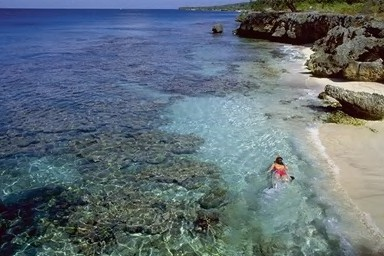
\includegraphics[width=\linewidth]{\detokenize{figuras/geracao/unsharp-a.png}}
      \caption{Original}
    \end{subfigure}
    \hspace{0.1\textwidth}
    \begin{subfigure}{.4\textwidth}
      \centering
      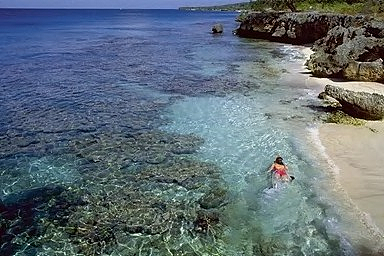
\includegraphics[width=\linewidth]{\detokenize{figuras/geracao/unsharp-b.png}}
      \caption{Imagem artificial}
    \end{subfigure}
  \end{center}
  \caption[Geração artificial utilizando unsharp masking.]{Geração artificial utilizando unsharp masking. \textit{Fonte:~Elaborado pela autora.}}
  \label{fig:gen:unsharp}
\end{figure}

\begin{description}
  \item[Parâmetros e suas variações] Pode-se variar o parâmetro $k$ de forma a ponderar a soma dessa diferença. Para a geração das imagens da classe minoritária, foi utilizado $k = 1$.

  \item[Limitações] É possível que existam pixels com valor negativo no resultado final. Isso pode causar o aparecimento de uma áurea em volta das bordas, efeito não desejado \cite{Gonzalez2007}.

  \item[Métodos relacionados] Outros algortimos de aguçamento conhecidos são: utilizar primeira derivada (grandiente) ou a segunda derivada da imagem (Laplaciano).

  \item[Visualização]
\end{description}
%%%%%%%%%%%%%%%%%%%%%%%%%%%%%%%%%%%%%%%%%%%%%%%%%%%%%%%%%%%%%%%%%%%%%%%%%%%%%%%%
\section{Adição de ruído}

O ruído de Poisson ocorre na contagem de fótons de dispositivos ópticos. Ele segue a distribuição de Poisson, que expressa a probabilidade de um certo número de eventos ocorrer em um intervalo fixo de tempo e/ou espaço se esses eventos ocorem com uma taxa média conhecida. O efeito da adição de ruído pode ser visto na Figura~\ref{fig:gen:noise}.

\begin{figure}[htbp]
  \begin{center}
    \begin{subfigure}{.4\textwidth}
      \centering
      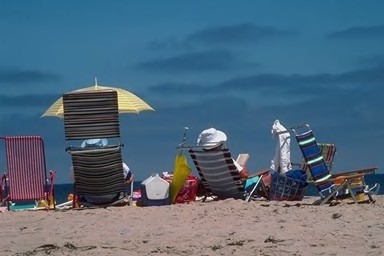
\includegraphics[width=\linewidth]{\detokenize{figuras/geracao/noise-a.png}}
      \caption{Original}
    \end{subfigure}
    \hspace{0.1\textwidth}
    \begin{subfigure}{.4\textwidth}
      \centering
      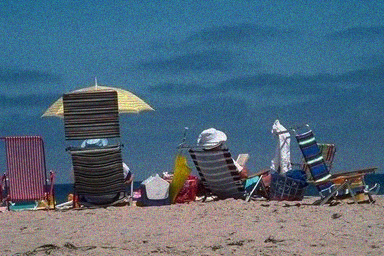
\includegraphics[width=\linewidth]{\detokenize{figuras/geracao/noise-b.png}}
      \caption{Imagem artificial}
    \end{subfigure}
  \end{center}
  \caption[Geração artificial utilizando adição de ruído de Poisson.]{Geração artificial utilizando adição de ruído de Poisson. \textit{Fonte:~Elaborado pela autora.}}
  \label{fig:gen:noise}
\end{figure}

\meutodo{descrever o algoritmo}

A distribuição de Poisson segue a equação:

% \begin{equation}
% $P_\mi)(n) = (e^(-\mi)\mi^(n))/(n!), n >= 0$
% \end{equation}

Uma possível implementação para encontrar os valores de Poisson foi desenvolvida por Knuth e pode ser vista no Algoritmo~\ref{alg:noise}.

\vspace{0.5cm}
\begin{algorithm}[H]
  \caption{Algoritmo da geração com ruído de Poisson}
  \label{alg:noise}
  \SetAlgoLined
  \Entrada{Imagem colorida $I$ em formato BGR}
  \Saida{Imagem gerada $G$}
  \ParaCada{pixel $(x,y)$}{
  $L \gets exp(-I(x,y))$\;
  $p \gets 1$\;
  $k \gets 0$\;
  \DoWhile{$p > L$}{
  $k \gets k + 1$\;
  $p \gets p * \text{número aleatório entre 0 e 1}$\;
  }
  $\text{G}(x,y) \gets k - 1$\;
  }
\end{algorithm}
\vspace{0.5cm}

\begin{description}
  \item[Parâmetros e suas variações]
  \item[Limitações] A adição de ruído é normalmente indesejável e a utilizamos
  para englobar mais um processamento de imagens. (??)
  \item[Métodos relacionados]
  \item[Visualização]
\end{description}
%%%%%%%%%%%%%%%%%%%%%%%%%%%%%%%%%%%%%%%%%%%%%%%%%%%%%%%%%%%%%%%%%%%%%%%%%%%%%%%%
\section{SMOTE visual}

Conforme visto na Seção \ref{sec:smote}, o SMOTE é um método de rebalanceamento aplicado após a extração de características. A ideia dessa geração, chamada de SMOTE visual, é imitar esse funcionamento no nível de pixels. A diferença é que não é feito entre as imagens mais próximas, mas sim entre duas imagens escolhidas de forma aleatória do conjunto de treinamento da classe minoritária.

Para cada pixel é calculado a diferença entre as duas imagens. Essa diferença é então multiplicada por um número aleatório no intervalo $[0-1]$ e adicionado
na imagem original (Ver Algoritmo~\ref{alg:smotevisual}). O efeito que esse processamento causa na imagem pode ser visualizado na Figura~\ref{fig:gen:smotevisual}.

\vspace{0.5cm}
\begin{algorithm}[H]
  \caption{Algoritmo da geração com SMOTE visual}
  \label{alg:smotevisual}
  \SetAlgoLined
  \Entrada{Imagem colorida $I$ em formato BGR}
  \Entrada{Imagem colorida $I_2$ em formato BGR}

  \Saida{Imagem gerada $G$}

  \ParaCada{pixel $(x,y)$} {
  $\text{diferença} \gets I(x,y) - I_2(x,y)$\;
  $\text{gap} \gets \text{número aleatório entre 0 e 1}$\;
  $\text{G}(x,y) \gets I(x,y) + gap*\text{diferença}$\;
  }

  $\text{mínimo} \gets \text{menor valor de G}$\;

  $\text{máximo} \gets \text{maior valor de G}$\;

  \ParaCada{pixel $(x,y)$} {
  $\text{G}(x,y) \gets G(x,y) - \text{mínimo}$\;
  }

  \ParaCada{pixel $(x,y)$} {
  $\text{G}(x,y) \gets G(x,y) * (255/(\text{máximo} - \text{mínimo}))$\;
  }
\end{algorithm}
\vspace{0.5cm}

\begin{figure}[htbp]
  \begin{center}
    \begin{subfigure}{.3\textwidth}
      \centering
      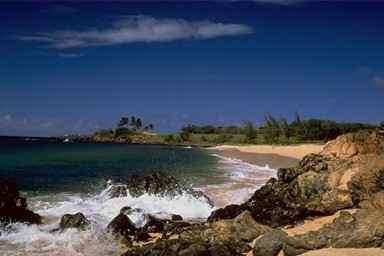
\includegraphics[width=\linewidth]{\detokenize{figuras/geracao/smote-a.png}}
      \caption{Original}
    \end{subfigure}
    \begin{subfigure}{.3\textwidth}
      \centering
      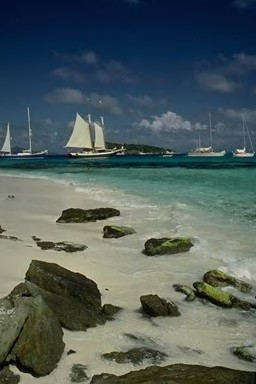
\includegraphics[width=0.65\linewidth]{\detokenize{figuras/geracao/smote-b.png}}
      \caption{Original}
    \end{subfigure}
    \begin{subfigure}{.3\textwidth}
      \centering
      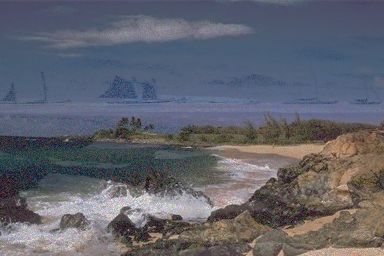
\includegraphics[width=\linewidth]{\detokenize{figuras/geracao/smote-c.png}}
      \caption{Imagem artificial}
    \end{subfigure}
  \end{center}
  \caption[Geração artificial utilizando o método SMOTE no espaço visual.]{Geração artificial utilizando o método SMOTE no espaço visual. \textit{Fonte:~Elaborado pela autora.}}
  \label{fig:gen:smotevisual}
\end{figure}

\begin{description}
  \item[Limitações] Esse método adiciona texturas e bordas que não estavam originalmente nas imagens.

  \item[Métodos relacionados] Esse método é visualmente parecido com o de mistura ponderada, apresentado na próxima seção.

  \item[Visualização]
\end{description}
%%%%%%%%%%%%%%%%%%%%%%%%%%%%%%%%%%%%%%%%%%%%%%%%%%%%%%%%%%%%%%%%%%%%%%%%%%%%%%%%
\section{Mistura ponderada}

Essa geração calcula a soma ponderada de duas imagens, de acordo com o
Algoritmo~\ref{alg:blend}. O efeito dessa mistura pode ser visto na Figura~\ref{fig:gen:blend}, onde dadas duas imagens como entrada, a imagem da direita corresponde a soma delas.

\begin{algorithm}[H]
  \vspace{0.5cm}
  \caption{Algoritmo de mistura ponderada}
  \label{alg:blend}
  \SetAlgoLined
  \Entrada{Primeira imagem colorida $I$ em formato BGR}
  \Entrada{Segunda imagem colorida $I_2$ em formato BGR}

  \Saida{Imagem gerada $G$}

  {$\alpha \gets \text{número aletatório entre 10 e 80}$\;}
  {$\beta \gets 100 - \alpha$\;}

  \ParaCada{pixel $(x,y)$} {
  $\text{G}(x,y) \gets \beta.I(x,y) + \alpha.I_2(x,y)$\;
  }
\end{algorithm}
\vspace{0.5cm}

\begin{figure}[htbp]
  \begin{center}
    \begin{subfigure}{.3\textwidth}
      \centering
      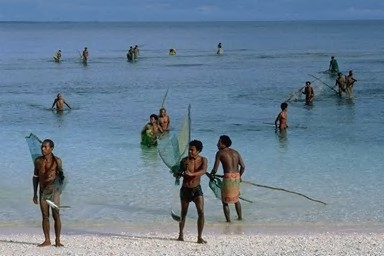
\includegraphics[width=\linewidth]{\detokenize{figuras/geracao/blend-a.png}}
      \caption{Original}
    \end{subfigure}
    \begin{subfigure}{.3\textwidth}
      \centering
      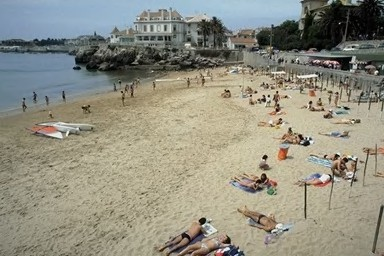
\includegraphics[width=\linewidth]{\detokenize{figuras/geracao/blend-b.png}}
      \caption{Original}
    \end{subfigure}
    \begin{subfigure}{.3\textwidth}
      \centering
      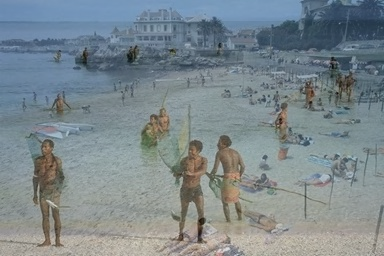
\includegraphics[width=\linewidth]{\detokenize{figuras/geracao/blend-c.png}}
      \caption{Imagem artificial}
    \end{subfigure}
  \end{center}
  \caption[Geração artificial utilizando uma mistura ponderada de duas imagens.]{Geração artificial utilizando uma mistura ponderada de duas imagens. \textit{Fonte:~Elaborado pela autora.}}
  \label{fig:gen:blend}
\end{figure}

\begin{description}
  \item[Parâmetros e suas variações] Os parâmetros $\alpha$ e $\beta$ são escolhidos de forma aleatória. Um valor entre 10\% e 80\% é escolhido para $\alpha$; e o $\beta$ é o restante para completar 100\%.

  \item[Limitações] Assim como todas as gerações artificiais que envolvem a mistura de imagens, efeitos são adicionados às imagens originais. Dependendo da combinação dos métodos de descrição, quantização e classificação, isso pode piorar a acurácia da classificação.

  \item[Métodos relacionados] É um método de combinação de imagens primitivo. Algoritmos similares são muito mais complexos, como os de threshold e saliência descritos a seguir.

  \item[Visualização]

\end{description}
%%%%%%%%%%%%%%%%%%%%%%%%%%%%%%%%%%%%%%%%%%%%%%%%%%%%%%%%%%%%%%%%%%%%%%%%%%%%%%%%
\section{Mistura limiarizada}

A combinação de \textit{thresholds} é uma composição do fundo (\textit{background}) de uma imagem e do objeto da cena (\textit{foreground}) de outra imagem. A Figura~\ref{fig:gen:threshold} mostra a mistura dos \textit{thresholds} de duas imagens originais para compor uma nova imagem. O Algoritmo~\ref{alg:threshold} descreve as operações necessárias para realizar tal processamento.

\begin{figure}[htbp]
  \begin{center}
    \begin{subfigure}{.3\textwidth}
      \centering
      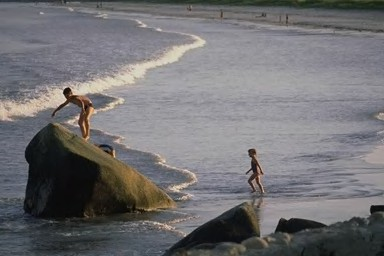
\includegraphics[width=\linewidth]{\detokenize{figuras/geracao/threshold-a.png}}
      \caption{Original}
    \end{subfigure}
    \begin{subfigure}{.3\textwidth}
      \centering
      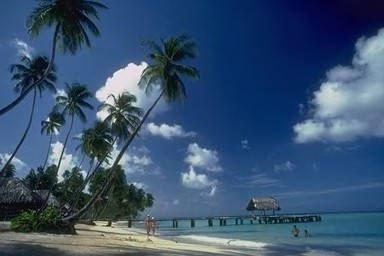
\includegraphics[width=\linewidth]{\detokenize{figuras/geracao/threshold-b.png}}
      \caption{Original}
    \end{subfigure}
    \begin{subfigure}{.3\textwidth}
      \centering
      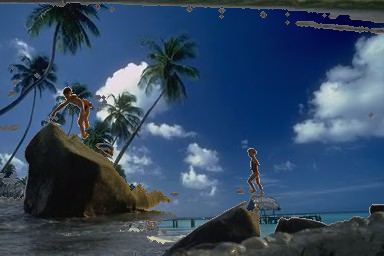
\includegraphics[width=\linewidth]{\detokenize{figuras/geracao/threshold-c.png}}
      \caption{Imagem artificial}
    \end{subfigure}
  \end{center}
  \caption[Geração artificial utilizando uma mistura limiarizada de duas imagens.]{Geração artificial utilizando uma mistura limiarizada de duas imagens. \textit{Fonte:~Elaborado pela autora.}}
  \label{fig:gen:threshold}
\end{figure}

\vspace{0.5cm}
\begin{algorithm}[H]
  \caption{Algoritmo de mistura limiarizada}
  \label{alg:threshold}
  \SetAlgoLined
  \Entrada{Imagem colorida $I$ em formato BGR}
  \Entrada{Imagem colorida $I_2$ em formato BGR}
  \Saida{Imagem gerada $G$}

  $I_{cinza} \gets \text{escala de cinza}(I)$\;
  $I_{threshold} \gets OTSU(I_{cinza})$\;
  $I_{morfologica} \gets \text{abertura e dilatação} (I_{threshold})$\;
  $I_{foreground} \gets \text{aplica máscara}(I_{morfologica}, I) $\;
  $I_{morfologica} \gets \text{oposto}(I_{morfologica})$\;
  $I_{background} \gets \text{aplica máscara}(I_{morfologica}, I_2) $\;
  $G \gets I_{background} + I_{foreground}$\;
\end{algorithm}
\vspace{0.5cm}

\begin{description}
  \item[Parâmetros e suas variações] No âmbito desta pesquisa, os parâmetros estão fixos, mas é possível modificar o tamanho dos elementos estruturantes que fazem as operações de abertura e dilação para remover pequenas regiões.

  \item[Limitações] Dependendo da quantidade de informações da imagem, o \textit{threshold de OTSU} pode não conseguir extrair nenhuma informação relevante ou mesmo a imagem toda.

  \item[Métodos relacionados] Essa geração está fortemente correlacionada com a mistura a partir da saliência da imagem, apresentada a seguir.

  \item[Visualização]
\end{description}
%%%%%%%%%%%%%%%%%%%%%%%%%%%%%%%%%%%%%%%%%%%%%%%%%%%%%%%%%%%%%%%%%%%%%%%%%%%%%%%%
\section{Mistura saliente}

A combinação de regiões salientes é muito similar com o método anterior de combinação de \textit{thresholds}, porém, utiliza um algoritmo mais robuscado que detecta a saliência da imagem a partir do método SLIC. A Figura~\ref{fig:gen:saliency} mostra a combinação da região saliente da imagem original à esquerda com a imagem central, resultando na imagem combinada à direita.

\begin{figure}[htbp]
  \begin{center}
    \begin{subfigure}{.3\textwidth}
      \centering
      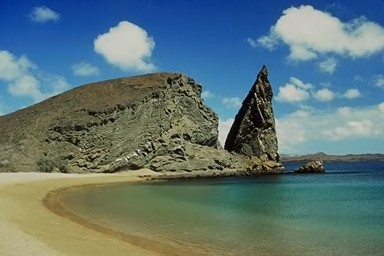
\includegraphics[width=\linewidth]{\detokenize{figuras/geracao/saliency-a.png}}
      \caption{Original}
    \end{subfigure}
    \begin{subfigure}{.25\textwidth}
      \centering
      \includegraphics[width=\linewidth]{\detokenize{figuras/geracao/saliency-b.png}}
      \caption{Original}
    \end{subfigure}
    \begin{subfigure}{.25\textwidth}
      \centering
      \includegraphics[width=\linewidth]{\detokenize{figuras/geracao/saliency-c.png}}
      \caption{Imagem artificial}
    \end{subfigure}
  \end{center}
  \caption[Geração artificial utilizando uma mistura de duas imagens a partir da saliência da primeira imagem.]{Geração artificial utilizando uma mistura de duas imagens a partir da saliência da primeira imagem. \textit{Fonte:~Elaborado pela autora.}}
  \label{fig:gen:saliency}
\end{figure}

As operações aplicadas na imagem para extrair a região mais saliente são: SLIC; rotulação por conectividade; \textit{threshold de OTSU}; e operações morfológicas. O Algoritmo~\ref{alg:saliency} apresenta os passos para o cálculo do \textit{background} e \textit{foreground}.

\vspace{0.5cm}
\begin{algorithm}[H]
  \caption{Algoritmo de mistura saliente}
  \label{alg:saliency}
  \SetAlgoLined
  \Entrada{Imagem colorida $I$ em formato BGR}
  \Entrada{Imagem colorida $I_2$ em formato BGR}
  \Saida{Imagem gerada $G$}

  $I_{\text{rotulada por segmento}} \gets SLIC(I)$\;
  $I_{\text{mapa de saliência}} \gets \text{rotulação por conectividade}(I_{\text{rotulada por segmento}})$\;
  $I_{threshold} \gets OTSU(I_{\text{mapa de saliência}})$\;
  $I_{morfologica} \gets \text{abertura e dilatação} (I_{threshold})$\;
  $I_{foreground} \gets \text{aplica máscara}(I_{morfologica}, I) $\;
  $I_{morfologica} \gets \text{oposto}(I_{morfologica})$\;
  $I_{background} \gets \text{aplica máscara}(I_{morfologica}, I_2) $\;
  $G \gets I_{background} + I_{foreground}$\;
\end{algorithm}
\vspace{0.5cm}

\begin{description}
  \item[Parâmetros e suas variações] Assim como no método anterior, os parâmetros são relacionados ao tamanho do elemento estruturante para a abertura e dilatação e estão fixos.

  \item[Limitações] Não é garantido que o algoritmo de saliência consiga extrair
  a melhor região, ou mesmo que sempre haja uma região.

  \item[Métodos relacionados] Similar à mistura por \textit{thresholds}.

  \item[Visualização]
\end{description}
%%%%%%%%%%%%%%%%%%%%%%%%%%%%%%%%%%%%%%%%%%%%%%%%%%%%%%%%%%%%%%%%%%%%%%%%%%%%%%%%
\section{Composição}

Essa geração pretende compor informações de diversas imagens em uma única imagem. Assim é feito um mosaico com várias imagens, conforme pode ser visto na  Figura~\ref{fig:gen:composition}. Se as imagens possuem um elemento centralizado, essa geração pode resultar em uma imagem de um objeto que parece uma mutação dos objetos centrais, conforme pode ser visualizado na Figura~\ref{}.

\begin{figure}[htbp]
  \begin{center}
    \centering
    \includegraphics[width=0.4\linewidth]{\detokenize{figuras/geracao/composition.png}}
  \end{center}
  \caption[Geração artificial utilizando uma composição de imagens.]{Geração artificial utilizando uma composição de imagens. \textit{Fonte:~Elaborado pela autora.}}
  \label{fig:gen:composition}
\end{figure}

Para cada quadrado a ser preenchido sorteia uma imagem do conjunto de treinamento, realiza uma operação de borramento, aguçamento, mistura ponderada ou visual SMOTE e adiciona essa imagem no quadrado respectivo. Os passos para tal composição estão descritos no Algoritmo~\ref{alg:composition}.

\vspace{0.5cm}
\begin{algorithm}[H]
  \caption{Algoritmo de composição}
  \label{alg:composition}
  \SetAlgoLined
  \Saida{Imagem gerada $G$}
  \Enqto{total < \text{número de quadrados $q$}}{
  $I \gets \text{imagem aleatória do conjunto de treinamento}$\;
  $\text{operação} \gets 1 + (rand() \% 3 )$\;
  \Selec{\text{operação}} {
  \uCaso{1} {
  $I \gets borramento(I)$\;
  }
  \uCaso{2} {
  $I \gets \text{mistura ponderada}(I)$\;
  }
  \uCaso{3} {
  $I \gets \text{aguçamento}(I)$\;
  }
  \uCaso{4} {
  $I \gets \text{visual SMOTE}(I)$\;
  }
  }
  $x \gets \text{posição aleatória em x de I}$\;
  $y \gets \text{posição aleatória em y de I}$\;
  $qx \gets \text{posição atual para o quadrado em x de G}$\;
  $qy \gets \text{posição atual para o quadrado em y de G}$\;
  $G(qx, qy) \gets I(x,y)$\;
  $total++$\;
  }
\end{algorithm}
\vspace{0.5cm}

\begin{description}
  \item[Parâmetros e suas variações] O parâmetro $q$ controla quantos quadrados serão criados na nova imagem. Nesta pesquisa foram realizados testes com 4 e 16.

  \item[Limitações] O término brusco de uma imagem para início da outra ao formar a grade de imagens tenha efeitos colaterais de inserção de textura que não excedam a vantagem de compor uma mesma imagem com várias cores, texturas e formas das imagens originais.

  \item[Métodos relacionados]

  \item[Visualização]
\end{description}
%%%%%%%%%%%%%%%%%%%%%%%%%%%%%%%%%%%%%%%%%%%%%%%%%%%%%%%%%%%%%%%%%%%%%%%%%%%%%%%%
% \section{Metodologia}
%
% \begin{description}
%  \item[Pesquisa bibliográfica:] \
%
%   \begin{enumerate}
% \item \underline{Características latentes}: são estudados diversos métodos de pré-processamento de imagens, como filtros de borramento e filtragem, com o objetivo de obter imagens processadas que sejam melhor caracterizadas para a etapa de classificação. O enfoque está em como realçar determinadas características, como, por exemplo, cor e textura, utilizando diversos algoritmos sobre as imagens originais.
%
% \item \underline{Redes neurais}: por representarem o estado da arte da classificação, reconhecimento e localização de objetos, as redes neurais de convolução são estudadas. Pretende-se utilizar a análise dos resultados do seu treinamento para identificar as características relevantes em imagens. Já as máquinas de Boltzmann restritas são redes neurais mais simples, portanto convenientes para a verificação da relevância de uma imagem para o aprendizado.
%
% \item \underline{Desbalanceamento de classes}: esse problema é fundamentado em reconhecimento de padrões, e consiste em lidar com um conjunto de classes que possuem quantidades desiguais de imagens. Deve-se assim pesquisar métodos que visam equilibrar o número de imagens em cada classe.
%
% \item \underline{Descritores}: são investigados métodos capazes de descrever as propriedades das imagens, como histograma global de cor (GCH)~\cite{Gonzalez2007}, vetor de coerência de cor (CCV)~\cite{ccv}, classificação de pixels de borda e interior (BIC)~\cite{bic}, auto-correlograma de cor (ACC)~\cite{acc} e descritores de Haralick~\cite{Haralick1973}.
%
% \item \underline{Classificador de padrões}: alguns classificadores fundamentados na literatura para a classificação de imagens são o Naive Bayes, OPF (\textit{Optimum-Path Forest}), KNN (\textit{K-Nearest Neighbor}), SVM (\textit{Support Vector Machines}) e Softmax. A depender da performance do sistema após experimentos um destes será escolhido. É importante destacar que esse não é o foco deste estudo, que tem a maior contribuição na pesquisa do pré-processamento das imagens de forma a obter características relevantes e no rebalanceamento de classes com dados de informação visual.
%   \end{enumerate}
%
%  \item[Implementação:] a biblioteca \-OpenCV \cite{Intel2010} será utilizada para as funções gerais de carregar, processar, salvar e classificar imagens. A linguagem de programação para utilizar esta biblioteca e na qual esta pesquisa está sendo implementada é C++. Para a geração de gráficos das medidas estatísticas a linguagem de programação Python é utilizada. O código está disponível em \url{https://bitbucket.org/moacirponti/imagefeatureextraction/overview}.
%
%  \item[Bases de imagens:] considerando que os objetivos propostos possuem um viés genérico, os experimentos vão ser realizados em diversas coleções de imagens com o objetivo de estabelecer ou refutar as hipóteses levantadas.
%
%  Os resultados preliminares foram obtidos utilizando a base de imagens COREL\footnote{Disponível em http://wang.ist.psu.edu/docs/related/}, composta por fotografias que representam as classes: tribos africanas, praia, construções, ônibus, dinossauros, elefantes, flores, cavalos, montanhas e tipos de comidas. São 10 classes balanceadas com 100 imagens cada. Para fins de exemplificação, foram selecionadas imagens que representam essas classes na Figura \ref{fig:corel}.
%
%  \begin{figure}[hbpt]
%  \begin{center}
%    \includegraphics[width=1\linewidth]{\detokenize {figuras/exemplos_corel.png}}
%  \end{center}
%   \caption[Base de imagens COREL-1000.]{Base de imagens COREL-1000 utilizada. Estão representadas as 10 classes da base. \textit{Fonte: Elaborado pela autora.}}
%  \label{fig:corel}
% \end{figure}
%
%
%  \item[Experimentos:] serão realizados diversos experimentos direcionados a explorar as etapas de pré-processamento, para melhorar a acurácia da classificação de bases de imagens. Como entrada são utilizadas imagens originais provenientes de diversas coleções disponíveis na literatura. Como resultado, serão calculadas medidas estatísticas da classificação dessas coleções após a alteração dessas imagens com os métodos de realce de características relevantes.
%
%  \item[Análise dos dados:] os experimentos realizados irão resultar em medidas estatísticas da classificação. A análise irá comparar a classificação das imagens originais com aquelas tratadas pelo método proposto. Ainda, o método de rebalanceamento de classes será comparado com técnicas disponíveis na literatura, como o SMOTE.
%
% \item[Forma de avaliação:] a medida estatística mais comum para avaliação é a razão do número de acertos pela quantidade de imagens testadas. Essa medida, conhecida por \underline{acurácia}, pode não refletir propriamente os resultados, em um cenário de bases desbalanceadas. Isso se deve ao fato de que se a classe minoritária não obtiver nenhum resultado correto e a classe majoritária tiver 100\% de acertos, a acurária normal poderá ser muito alta, mesmo considerando que nenhuma imagem da classe minoritária foi corretamente classificada. Dessa forma, considera que os erros são igualmente importantes. Mas em se tratando de bases desbalanceadas, deve-se diferenciar o erro em, por exemplo, diagnosticar um paciente doente -- classe minoritária -- como sendo saudável e um paciente saudável -- classe majoritária -- como estando doente \cite{Batista2004}. No primeiro caso, o paciente corre risco de diagnóstico tardil, enquanto o paciente saudável realiza outros testes para refutação.
%
% Pode-se estender essa medida obtendo-se a \underline{acurácia $k$-fold}: medida de acerto baseada na divisão do conjunto de objetos em teste e treinamento, realizando a repetição dos experimentos $n$ vezes e obtendo a média e o desvio padrão. A acurácia de cada experimento é obtida pela Equação~\ref{eq:Accuracy}, que considera problemas de desbalanceamento de classes.
%
%     \begin{equation}
%       Acc = 1 - \frac{\sum_{i=1}^{c} E(i)}{2c},
%     \label{eq:Accuracy}
%     \end{equation}
%
%     \noindent onde $c$ é o número de classes e $E(i) = e_{i,1} + e_{i,2}$ é o erro relativo a $c$, calculado por:
%
%     \begin{equation*}
%       e_{i,1} = \frac{FP(i)}{N-N(i)} \,\,\,\,\, \text{ e } \,\,\,\,\, e_{i,2} = \frac{FN(i)}{N(i)}, i=1,...,c,
%     \label{eq:Errors}
%     \end{equation*}
%    \noindent onde $FN(i)$ (falsos negativos) são os exemplos pertencentes a $i$ e incorretamente classificados, e $FP(i)$ (falsos positivos) são os exemplos erroneamente rotulados como~$i$.
%
% % consideramos positivos a minoritaria
%
% Uma outra medida para bases desbalanceadas é a \underline{medida-F1} (conhecida como \textit{F1-Measure} ou \textit{F1-Score} e apresentada na Equação~\eqref{medidaf}), que combina precisão e revocação como medida de efetividade da classificação \cite{Garcia2009}.
% % Pode efetivamente avaliar a performance de classificação em cenários desbalanceados.
% A precisão (Equação~\ref{precisao}) é a medida da exatidão: dos exemplos classificados como positivos, quantos realmente são. E a revocação (Equação~\ref{revocacao}) é a medida de completude: quantos exemplos positivos foram corretamente classificados como tal.
%
% \begin{equation}
%   P = \frac{VP}{VP + FP},
%   \label{precisao}
% \end{equation}
%
% \noindent onde $VP$ são os exemplos positivos corretamente classificados.
%
% \begin{equation}
%   R = \frac{VP}{VP + FN}
%   \label{revocacao}
% \end{equation}
%
% \begin{equation}
%   F1 = 2 \frac{PR}{P+R}
%   \label{medidaf}
% \end{equation}
%
% A partir dessas medidas, o \underline{teste estatístico de Friedman} pode ser usado para determinar se há diferença significante em uma amostra de resultados gerados \cite{friedman2010}. As performances dos algoritmos são analisados e um \textit{rank} é atribuído para cada conjunto de dados. Ele considera que a hipótese nula a ser testada é que não há diferença estatística relevante entre as observações. Para analisar se o teste da hipótese é significativo, pode ser utilizado o \underline{p-valor}, que indica o quão estatisticamente significante o resultado é: quanto menor o seu valor, maior a evidência contra a hipótese nula (geralmente o limiar utilizado é de 0,05).
%
% Por fim, a \underline{distância de Mahalanobis} também pode ser utilizada: antes e depois da geração artificial de imagens, calcular a distância entre a média das classes e a variância dentro das classes \cite{mahalanobis2000}. Ela se baseia na correlação entre as variáveis e pode ser definida por
% \begin{equation*}
%   D_m(x_i) = \sqrt{(x_i - \mu)C^{-1}(x_i-\mu)^T},
% \end{equation*}
% \noindent onde $x_i$ é um vetor de valores, $\mu$ a média e C a matriz de covariância.
%
% \end{description}
%
% %--------------------------------------------------------------------------------
% \section{Resultados esperados}
% \label{sec:resultados}
%
% Os resultados esperados são relacionados às áreas de \textbf{processamento de imagens e reconhecimento de padrões}. Espera-se obter uma comprovação das hipóteses levantadas por essa pesquisa. Os resultados são esperados em duas vertentes:
%
% \begin{enumerate}
%  \item \textit{Pré-processamento} de imagens que caracterizem melhor aspectos de suas classes, aumentando a variância entre as classes quando comparado com as imagens originais.
%  \item \textit{Geração artificial de imagens} de classes minoritárias de forma a compensar o desbalanceamento natural das bases de dados.
% \end{enumerate}
%
% Em ambos os casos pretende-se melhorar a classificação, validando-a através do cálculo da medida-F1. A análise das características aprendidas por uma rede neural de convolução será realizada ao executar o treinamento com bases específicas que destaquem propriedades como cor, textura e forma. Além disso, os resultados serão obtidos a partir da escolha de quais imagens adicionam informação ao conjunto de treino. As redes RBM serão utilizadas para este fim. Bases naturalmente não balanceadas serão testadas e seus resultados avaliados.


%--------------------------------------------------------------------------------
\section{Considerações finais}

% A proposta desta pesquisa foi apresentada, descrevendo a sua metodologia. Foi dado destaque aos resultados esperados e à forma de avaliação, descrevendo as medidas estatísticas a serem utilizadas. O cronograma previsto para a realização deste mestrado foi destacado, elencando as atividades e suas respetivas durações. O próximo capítulo apresentará os resultados preliminares.


\chapter{Resultados: Quantização de Imagens}
\label{cap:resultados-quantizacao}
% \meutodo{
%   Variação gradual de parâmetros para identificar o que causa perdas/ganhos
% }

%%%%%%%%%%%%%%%%%%%%%%%%%%%%%%%%%%%%%%%%%%%%%%%%%%%%%%%%%%%%%%%%%%%%%%%%%%%%%%%%
\section{Considerações Iniciais}

Este capítulo apresenta os resultados encontrados quando os métodos de quantização de imagens foram aplicados no pipeline de reconhecimento de imagens. Para cada experimento realizado, são descritos: a base de imagens, o protocolo utilizado, os resultados encontrados e a discussão da relevância de tais resultados.

Os experimentos são relacionados à quantização de imagens, quando realizada antes da extração de características, e portanto no campo visual. Os resultados devem refletir melhoras nas etapas subsequentes, como uma melhor acurácia na etapa de classificação ou a redução do tempo de processamento.

%%%%%%%%%%%%%%%%%%%%%%%%%%%%%%%%%%%%%%%%%%%%%%%%%%%%%%%%%%%%%%%%%%%%%%%%%%%%%%%%
\section{Experimentos}

O objetivo dessa seção é mostrar os efeitos da etapa de quantização e como ela pode ser utilizada para reduzir a dimensionalidade do espaço de características. A Figura \ref{fig:quant:flowResult} demonstra o fluxo das operações e os métodos utilizados nos experimentos. Inicialmente, as imagens foram quantizadas em 256, 128, 64, 32 e 16 cores. Após, suas características foram extraídas e duas etapas de experimentos são realizadas:

\begin{enumerate}
  \item Experimentos utilizando um método de extração de características seguido pela classificação (sem posterior seleção de características);
  \item Experimentos utilizando o vetor resultante da concatenação de todos os métodos de extração, seguido pela classificação com e sem a seleção de características.
\end{enumerate}

\begin{figure}[!htbp]
  \begin{center}
    \centering
    \includegraphics[width=0.4\linewidth]{\detokenize{figuras/quantizacao/quantizationResult.pdf}}
  \end{center}
  \caption[Essa figura demonstra o fluxo das operações e os métodos utilizados nos experimentos. Após a aquisição da imagem, ela é convertida para escala de cinza por algum método de quantização e seus níveis de cor reduzidos por um parâmetro de quantização. Dependendo do método, a correção \emph{gamma} é realizada. A imagem quantizada serve então como entrada para um método de extração de características e posteriormente é classificada com \emph{SVM}. Uma das etapas de experimentos prevê também a concatenação de todos os vetores extraídos e a seleção das características com \emph{LPP} antes da classificação.]{Essa figura demonstra o fluxo das operações e os métodos utilizados nos experimentos. Após a aquisição da imagem, ela é convertida para escala de cinza por algum método de quantização e seus níveis de cor reduzidos por um parâmetro de quantização. Dependendo do método, a correção \emph{gamma} é realizada. A imagem quantizada serve então como entrada para um método de extração de características e posteriormente é classificada com \emph{SVM}. Uma das etapas de experimentos prevê também a concatenação de todos os vetores extraídos e a seleção das características com \emph{LPP} antes da classificação. \textit{Fonte:~Elaborado pela autora.}}
  \label{fig:quant:flowResult}
\end{figure}

%%%%%%%%%%%%%%%%%%%%%%%%%%%%%%%%%%%%%%%%%%%%%%%%%%%%%%%%%%%%%%%%%%%%%%%%%%%%%%%%
\subsection{Base de Imagens}

Três bases de imagens, ilustradas na Figura~\ref{fig:quant:bases}, foram utilizadas nestes experimentos:
\begin{itemize}
\item[] \textbf{Corel-1000}\footnote{Disponível em http://www.wang.ist.psu.edu/docs/related/}: consiste em dez classes balanceadas de imagens naturais, com algumas classes bem definidas e algumas não;
\item[] \textbf{Caltech101-600}\footnote{Disponível em http://www.vision.caltech.edu/ImageDatasets/Caltech101/}: contém fotos e desenhos. Desta base, foi utilizado um conjunto de seis classes balanceadas: aviões, bonsais, candelabros, tartarugas, motocicletas e relógios;
\item[] \textbf{Produce}\footnote{Disponível em ??} (também conhecido como base de vegetais e frutas tropicais): composta por imagens com um fundo similar mas muitas mudanças na iluminação, no número de objetos e na escala. Apesar da oclusão parcial de objetos ser observada, essa classe possui dados bem comportados.
\end{itemize}

\begin{figure}[!htbp]
  \begin{center}
    \subfloat[Base de imagens Caltech101]{
      \includegraphics[width=\linewidth]{\detokenize{figuras/quantizacao/fig_Caltech101_dataset.jpg}}
    }
    \newline
    \subfloat[Base de imagens Corel-1000]{
      \includegraphics[width=\linewidth]{\detokenize{figuras/quantizacao/fig_COREL_dataset.jpg}}
    }
    \newline
    \subfloat[Base de imagens Produce]{
      \includegraphics[width=\linewidth]{\detokenize{figuras/quantizacao/fig_Produce_dataset.jpg}}
    }
  \end{center}
  \caption[Bases de imagens utilizadas para os experimentos de quantização.]{Bases de imagens utilizadas para os experimentos de quantização. \textit{Fonte:~\cite{Ponti2016}.}}
  \label{fig:quant:bases}
\end{figure}

Estes experimentos possuem foco na redução na dimensionalidade. Para evitar o problema do desbalanceamento, as bases \textit{Produce} e \textit{Caltech101} foram modificadas. Dessa forma, as classes disponíveis foram balanceadas ao remover imagens das classes majoritárias.

%%%%%%%%%%%%%%%%%%%%%%%%%%%%%%%%%%%%%%%%%%%%%%%%%%%%%%%%%%%%%%%%%%%%%%%%%%%%%%%%
\subsection{Protocolo}

Os experimentos foram realizados com uma validação cruzada de \textit{10-fold}. Considerando que as bases estão balanceadas e que a seleção de exemplos para a validação cruzada é estratificada, a medida estatística de \textit{acurácia} foi utilizada para avaliar a performance da classificação. O seguinte protocolo foi seguido para a obtenção dos resultados:

\begin{enumerate}
\item \textbf{Quantização}: com os métodos \emph{Intensidade}, \emph{Gleam}, \emph{Luminância} e \emph{MSB}.
\item \textbf{Extração de características}: utilizando os métodos -- e parâmetros escolhidos com base nas recomendações dos artigos que proporam tais métodos -- a seguir:
  \begin{itemize}
    \item \emph{ACC}: utilizando um conjunto de quatro distâncias $D = {1, 3, 5, 7}$ e a distância tabuleiro de xadrez $D_8(p,q) = Max(|x-s|, |y-t|)$ entre os pixeis $p(x,y)$ e $q(s,t)$;
    \item \emph{BIC}: com uma vizinhança de quatro pixels;
    \item \emph{CCV}: adotando um valor de $\mathit{threshold} = 25$ para a classificação dos pixels entre coerentes e incoerentes;
    \item \emph{Haralick-6}: o pixel vizinho para o qual computar a matriz de correlação foi definido como sendo o pixel à direita.
  \end{itemize}
\item \textbf{Redução da dimensionalidade}: a projeção LPP foi realizada com o parâmetro $k$ = 128, 64, 32 e 16 dimensões e 10 vizinhos. Esse parâmetro foi determinado empiricamente e não influencia consideravelmente a acurácia.
\item \textbf{Classificação}: com o classificador SVM (\textit{Support Vector Machines}). Os parâmetros para essa etapa foram encontrados utilizando uma \textit{grid search} no conjunto de treino.
\end{enumerate}

%%%%%%%%%%%%%%%%%%%%%%%%%%%%%%%%%%%%%%%%%%%%%%%%%%%%%%%%%%%%%%%%%%%%%%%%%%%%%%%%
\subsection{Resultados e Discussão}

A Figura \ref{fig:quant:results} ilustra a acurácia média para o primeiro conjunto de experimentos: para cada combinação de base de dados e método de extração, são demonstrados seis resultados de acurácia correspondentes à quantização para 256, 128, 64, 32, 16 e 8 cores. Com base nessa figura é possível identificar que o método para obter a imagem quantizada tem uma impacto significativo na acurácia da classificação. Além disso, a redução de 256 para um menor número de cores normalmente manteve as acurácias e em alguns casos resultou em uma ligeira melhora, especialmente para os níveis de 128 e 64.

\begin{figure}[!htbp]
  \begin{center}
    \centering
    \includegraphics[width=\linewidth]{\detokenize{figuras/quantizacao/fig_results_individual.png}}
  \end{center}
  \caption[Resultados para Corel(a), Produce(b) e Caltech(c), utilizando todos os métodos de quantização. Para cada método de extração de características a acurácia é resultante da sua aplicação utilizando 256, 128, 64, 32, 16 e 8 cores, da esquerda para a direita.]{Resultados para Corel(a), Produce(b) e Caltech(c), com todos os métodos de quantização. Para cada método de extração de características a acurácia é resultante da sua aplicação utilizando 256, 128, 64, 32, 16 e 8 cores, da esquerda para a direita.\textit{Fonte:~\cite{Ponti2016}.}}
  \label{fig:quant:results}
\end{figure}

A partir dessa análise geral, uma análise mais específica foi realizada com a combinação dos métodos BIC e MSB; e Haralick e Luminância. Considerando que a utilização de apenas 16 e 8 cores resultou em uma acurácia muito inferior, o restante dos resultados utilizam 256, 128, 64 e 32 cores.

\meutodo{descrever o teste estatístico e o resultado}

O teste estatístico ANOVA foi realizado para comparar as acurácias dos experimentos da Figura \ref{fig:quant:boxplotBIC} e \ref{fig:quant:boxplotHaralick}. O boxplot para 256, 128, 64 e 32 cores com os métodos BIC e MSB está demonstrado na Figura \ref{fig:quant:boxplotBIC}. De acordo com o teste estatístico representado, utilizar características de cor e níveis de quantização providos pelo método MSB demonstrou resultados melhores do que com 256 cores para as bases Corel (128, 64 e 32 cores) e Caltech (64 cores). O único resultado que piorou significativamente foi para 32 cores da base de imagens \textit{Produce}. Portanto, reduzir converter as imagens de 3 canais de cores para um e reduzir os 256 possíveis valores para apenas 64 provou uma boa escolha de processamento anterior a extração de características. Menores valores podem degradar os resultados em características de textura, como mostrado na Figura \ref{fig:quant:boxplotHaralick}.

\begin{figure}[!htbp]
  \begin{center}
    \centering
    \includegraphics[width=\linewidth]{\detokenize{figuras/quantizacao/fig_results_individual_boxplotBIC.png}}
  \end{center}
  \caption[Resultados de acurácia para o método de quantização MSB considerando 256, 128, 64 e 32 cores com o descritor BIC. Os boxplots em cinza correspondem às significâncias estatísticas com $p \l 0.01$ quando comparado a acurácia de 256 cores.]{Resultados de acurácia para o método de quantização MSB considerando 256, 128, 64 e 32 cores com o descritor BIC. Os boxplots em cinza correspondem às significâncias estatísticas com $p \l 0.01$ quando comparado a acurácia de 256 cores. \textit{Fonte:~\cite{Ponti2016}.}}
  \label{fig:quant:boxplotBIC}
\end{figure}

\begin{figure}[!htbp]
  \begin{center}
    \centering
    \includegraphics[width=\linewidth]{\detokenize{figuras/quantizacao/fig_results_individual_boxplotHaralick.png}}
  \end{center}
  \caption[Resultados de acurácia para o método de quantização Luminância considerando 256, 128, 64 e 32 cores com o descritor Haralick. Os boxplots em cinza correspondem às significâncias estatísticas com $p \l 0.01$ quando comparado a acurácia de 256 cores.]{Resultados de acurácia para o método de quantização Luminância considerando 256, 128, 64 e 32 cores com o descritor Haralick. Os boxplots em cinza correspondem às significâncias estatísticas com $p \l 0.01$ quando comparado a acurácia de 256 cores. \textit{Fonte:~\cite{Ponti2016}.}}
  \label{fig:quant:boxplotHaralick}
\end{figure}

A redução de dimensionalidade obtida utilizando os métodos de quantização e redução da dimensionalidade com o LPP está ilustrada na Figura \ref{fig:quant:boxplotMSBLPP}. A imagem de entrada foi convertida para escala de cinza com o método MSB em 256 cores. Essa imagem foi dada como entrada para o método de extração de características BIC, que resultou em um vetor dado como entrada para o LPP. Esse último passo teve o objetivo de produzir versões reduzidas desse vetor para 256, 128 e 64 dimensões. As acurácias obtidas foram comparadas com a classificação dos vetores reduzidos apenas pela quantização. O método de quantização obteve valores de acurácia menores à utilização do LPP em três experimentos: de 256 dimensões com a base \textit{Corel} e com 256 e 64 na base \textit{Produce}. Para a base \textit{Caltech} a quantização foi melhor com 256 e 128 dimensões. O restante dos experimentos não apresentaram diferença estatística relevante. Apesar da perda de acurácia em alguns casos, é importante notar que -- se utilizado um número de cores correto -- é possível manter ou até mesmo melhorar as acurácias após a redução da dimensionalidade. Isso pode ser observado na Figura \ref{fig:quant:boxplotMSBLPP} referente à base de dados \textit{Caltech}.

\begin{figure}[!htbp]
  \begin{center}
    \centering
    \includegraphics[width=\linewidth]{\detokenize{figuras/quantizacao/fig_results_individual_boxplotMSBLPP.png}}
  \end{center}
  \caption[Resultados de acurácia para os método MSB (quantização), LPP (redução de dimensionalidade) e BIC (extração de características). A comparação do LPP versus MSB foi realizada com a mesma dimensionalidade. Os boxplots em cinza correspondem às significâncias estatísticas com $p \l 0.01$ quando comparado a acurácia de 256 cores.]{Resultados de acurácia para os método MSB (quantização), LPP (redução de dimensionalidade) e BIC (extração de características). A comparação do LPP versus MSB foi realizada com a mesma dimensionalidade. Os boxplots em cinza correspondem às significâncias estatísticas com $p \l 0.01$ quando comparado a acurácia de 256 cores. \textit{Fonte:~\cite{Ponti2016}.}}
  \label{fig:quant:boxplotMSBLPP}
\end{figure}

O número de dimensões de um vetor resultante de apenas um método de extração de características pode ser considerado baixo. Ainda mais que é comum extrair diversos descritores para uma situação, considernado que normalmente não está claro qual método deveria ser utilizado em cada caso. Por conta disso, os próximos experimentos utilizaram a concatenação de tais características. O objetivo destes experimentos é verificar se a concatenação de todos os descritores pode melhorar os resultados de acurácia. Além disso, comparar os resultados com os experimentos anteriores, afim de verificar se a quantização pode ser uma alternativa a redução da dimensionalidade com métodos convencionais (LPP, neste caso). A melhor configuração encontrada, até então, entre tamanho do vetor e acurácia foi utilizando 128 e 64 cores.

Inicialmente, foi testada a configuração de um vetor $D=2310$ com LPP para redução de dimensionalidade com $d$ = 1160, 582, 294 e 150. Ou seja, produzindo vetores com o mesmo tamanho dos obtidos apenas com a quantização como redução da dimensão. O número de características em relação ao número de cores, concatenando todos os vetores resultantes dos métodos de extração de características, é: 256 cores -- 2310 características; 128 cores -- 1160 características; 64 cores -- 582 características; 32 cores --- 294 características; e 16 cores -- 150 características. A Figura \ref{fig:quant:resultsFull} mostra os resultados utilizando LPP. Note que o método de quantização MSB resultou em acurácias melhores que os outros métodos.

\begin{figure}[!htbp]
  \begin{center}
    \centering
    \includegraphics[width=\linewidth]{\detokenize{figuras/quantizacao/fig_results_full.png}}
  \end{center}
  \caption[Comparação da acurácia alcançada com diferentes métodos de quantização: Gleam, Intensidade, Luminância e MSB. Inicialmente com $D=2310$ e então reduzindo com LPP para $d = 1160$, $582$, $294$ e $150$.]{Comparação da acurácia alcançada com diferentes métodos de quantização: Gleam, Intensidade, Luminância e MSB. Inicialmente com $D=2310$ e então reduzindo com LPP para $d = 1160$, $582$, $294$ e $150$. \textit{Fonte:~\cite{Ponti2016}.}}
  \label{fig:quant:resultsFull}
\end{figure}

A utilização da concatenação de todos os vetores melhorou a acurácia em relação ao melhor descritor individual. A Figura \ref{fig:quant:resultsFullBoxplot} apresenta a comparação do espaço original com LPP e MSB para redução da dimensionalidade. O teste estatístico ANOVA foi realizado utilizando $\alpha = 0.01$ como nível de significância. Os resultados que não mudaram significativamente as acurácias foram: MSB com 582 características para a base de dados Corel; e MSB com 1160 nas três bases. O único resultado de piora significative foi para 32 cores com a base Produce. Por conta disso, 64 cores parece ser uma boa escolha de parâmetro de quantização.

\begin{figure}[!htbp]
  \begin{center}
    \centering
    \includegraphics[width=\linewidth]{\detokenize{figuras/quantizacao/fig_results_full_boxplot.png}}
  \end{center}
  \caption[Comparação da acurácia com o uso da projeção LPP e o método MSB para quantização das imagens com o objetivo de redução de dimensionalidade.]{Comparação da acurácia com o uso da projeção LPP e o método MSB para quantização das imagens com o objetivo de redução de dimensionalidade. \textit{Fonte:~\cite{Ponti2016}.}}
  \label{fig:quant:resultsFullBoxplot}
\end{figure}

Os resultados indicam que a quantização pode ser utilizada como redução da dimensão de dados visuais, especialmente utilziando 128 e 64 cores. Como experimento, a Figura \ref{fig:quant:fullLPP} mostra as acurácias resultantes da aplicação do LPP sob o vetor obtido após a quantização com MSB utilizando 256 e 64 cores ($d=2310$ e $d=582$, respectivamente). É interessante notar que as projeções LPP em geral foram melhores com as imagens quantizadas em 64 cores com MSB ao invés da original em 256. A razão para isso deve estar no fato da quantização remover informações confusas: ela simplifica as imagens de forma que as cores restantes possam melhor descrever uma certa classe.

\begin{figure}[!htbp]
  \begin{center}
    \centering
    \includegraphics[width=0.6\linewidth]{\detokenize{figuras/quantizacao/fig_results_full_LPP}}
  \end{center}
  \caption[Resultados para a projeção do LPP sobre o espaço de características produzido pelo método de quantização MSB utilizando 256 ($d = 2310$) e 64 cores ($d=582$)]{Resultados para a projeção do LPP sobre o espaço de características produzido pelo método de quantização MSB utilizando 256 ($d = 2310$) e 64 cores ($d=582$)\textit{Fonte:~\cite{Ponti2016}.}}
  \label{fig:quant:fullLPP}
\end{figure}

O vetor concatenado com todos os descritores possui $9C + 6$ dimensões, onde $C$ é o número de cores da imagem de entrada. E o tempo de execução para a extração de todas as características é $f(N) = 42N + 6C^2$, onde $N$ é o número de pixels. Para cada imagem são necessárias $D^2 + kD + d^2$ operações para computar o vetor reduzido com LPP, onde $D$ é o tamanho do vetor original, $d$ o tamanho do vetor de saída e $k$ é o número de vizinhos utilizados no algoritmo.

Ao comparar o uso da quantização com a utilização de métodos mais complexos para redução da dimensionalidade, esse procedimento permite uma redução significante, enquanto normalmente preserva ou melhora a acurácia do sistema. Independente da utilização de um método de seleção de características, ao escolher um método de quantização apropriado e seus parâmetros é possível reduzir a dimensionalidade e acelerar computacionalmente as etapas que precedem o reconhecimento de imagens. Considere o seguinte exemplo: 100 imagens com 256 cores demandam 231.6 milhões de instruções para extrair as características e reduzir o vetor utilizando o método LPP (com $k = 10$ e $d = 50$). Se ao invés disso, fossem utilizadas 64 cores, esse número cairia para 58.7 milhões, o que corresponde a uma redução de 74,6\%.

\section{Considerações Finais}


\chapter{Resultados: Geração Artificial de Imagens}
\label{cap:resultados-geracao}

% \item \emph{ACC}: com um conjunto de quatro distâncias $D = {1, 3, 5, 7}$ e a distância tabuleiro de xadrez $D_8(p,q) = Max(|x-s|, |y-t|)$ entre os pixeis $p(x,y)$ e $q(s,t)$;
% \item \emph{BIC}: com uma vizinhança de quatro pixels;
% \item \emph{CCV}: adotando um valor de $\mathit{threshold} = 25$ para a classificação dos pixels entre coerentes e incoerentes;
% \item \emph{Haralick-6}: o pixel vizinho para o qual computar a matriz de correlação foi definido como sendo o pixel à direita.

%%%%%%%%%%%%%%%%%%%%%%%%%%%%%%%%%%%%%%%%%%%%%%%%%%%%%%%%%%%%%%%%%%%%%%%%%%%%%%%%
\section{Considerações Iniciais}

Os resultados encontrados ao rebalancear classes a partir da geração de imagens artificiais são apresentados neste capítulo. Para cada experimento realizado, são descritos: o protocolo utilizado (i.e. base de imagens e os métodos de conversão para escala de cinza e extração de características), os resultados encontrados e a discussão da relevância de tais resultados.

Foram realizados diversos experimentos direcionados a explorar o rebalanceamento com métodos de processamento, para melhorar a acurácia da classificação de bases de imagens. Como entrada são utilizadas imagens provenientes de diversas coleções disponíveis na literatura. Como resultado, são calculadas medidas estatísticas da classificação dessas bases de imagens após o rebalanceamento destas. Tal processamento é realizado antes da extração de características, e portanto no campo visual. Espera-se que os resultados encontrados proporcionem melhoras na etapa subsequente de classificação.

\meutodo{Nesse capítulo, falta ainda discutir melhor os resultados.}

%%%%%%%%%%%%%%%%%%%%%%%%%%%%%%%%%%%%%%%%%%%%%%%%%%%%%%%%%%%%%%%%%%%%%%%%%%%%%%%%

\section{Experimentos}

Essa seção descreve os resultados encontrados ao rebalancear as classes de imagens aplicando os processamentos -- descritos no Capítulo \ref{cap:metodo} -- nas imagens originais. As imagens geradas são então utilizadas como treinamento da classe minoritária. A Figura \ref{fig:fluxo} destaca o fluxo de operações realizadas para a análise do impacto da geração de imagens no rebalanceamento de classes. O mesmo protocolo de conversão para escala de cinza, extração de características e classificação foi seguido para três sub-experimentos: base desbalanceada; base rebalanceada com interpolação dos vetores de características (método SMOTE); e base rebalanceada com a geração artificial de imagens. Alguns experimentos foram realizados com bases de imagens originalmente balanceadas. Para tais casos, foi necessário desbalancear a base para testar o rebalanceamento.

\begin{figure}[!htbp]
\centering
\includegraphics[scale=1.1]{\detokenize{figuras/flow_main.pdf}}
\caption[Fluxo de operações para obtenção dos resultados do rebalanceamento de classes]{Fluxo de operações para obtenção dos resultados do rebalanceamento de classes. \textit{Fonte:~Elaborado pela autora.}}
\label{fig:fluxo}
\end{figure}

Procurando estabilidade dos resultados obtidos com a geração das imagens artificiais, foi identificada a necessidade de controlar a remoção de imagens da base no momento da criação da base desbalanceada. Assim, os resultados foram obtidos a partir de uma forma de validação \textit{K-fold} com o objetivo de prover mais robustez ao sistema. A Figura \ref{fig:folds} ilustra como tal validação é realizada, utilizando como exemplo uma base com duas classes de imagens. Primeiramente as imagens são separadas de forma aleatória em $k = 5$ \textit{folds} em cada classe. Em seguida, as duas classes compõem 40 configurações, consistindo em todas as possibilidades de: um fold para teste e os outros como treino para a classe que permanecerá balanceada; e um de teste e apenas um de treino para a classe que os métodos de processamento irão rebalancear. Tal validação é repetida para todas as classes, ou seja, cada classe tem a possibilidade de ser a minoritária. Se originalmente a base é naturalmente desbalanceada, um \textit{fold} é utilizado para teste e os demais como treino para todas as classes.

\begin{figure}[!htbp]
\centering
\includegraphics[scale=0.3]{\detokenize{figuras/folds_chart.png}}
\caption[]{\textit{Fonte:~Elaborado pela autora.}}
\label{fig:folds}
\end{figure}

\meutodo{Tenho que escrever o caption}

A medida estatística mais comum para avaliação é a razão do número de acertos pela quantidade de imagens testadas. Essa medida, conhecida por \underline{acurácia}, pode não refletir propriamente os resultados em um cenário de bases desbalanceadas. Isso se deve ao fato de que se a classe minoritária não obtiver nenhum resultado correto e a classe majoritária tiver 100\% de acertos, tal acurária poderá ser muito alta, mesmo considerando que nenhuma imagem da classe minoritária foi corretamente classificada. Dessa forma, considera que os erros são igualmente importantes. Mas em se tratando de bases desbalanceadas, deve-se diferenciar o erro em, por exemplo, diagnosticar um paciente doente -- classe minoritária -- como sendo saudável e um paciente saudável -- classe majoritária -- como estando doente \cite{Batista2004}. No primeiro caso, o paciente corre risco de diagnóstico tardil, enquanto o paciente saudável realiza outros testes para refutação.

Pode-se estender essa medida obtendo-se a \underline{acurácia $k$-fold}: medida de acerto baseada na divisão do conjunto de objetos em teste e treinamento, realizando a repetição dos experimentos $n$ vezes e obtendo a média e o desvio padrão. A acurácia de cada experimento é obtida por

    \begin{equation*}
      Acc = 1 - \frac{\sum_{i=1}^{c} E(i)}{2c},
    \label{eq:Accuracy}
    \end{equation*}

    \noindent  que considera problemas de desbalanceamento de classes, onde $c$ é o número de classes e $E(i) = e_{i,1} + e_{i,2}$ é o erro relativo a $c$, calculado por

    \begin{equation*}
      e_{i,1} = \frac{FP(i)}{N-N(i)} \,\,\,\,\, \text{ e } \,\,\,\,\, e_{i,2} = \frac{FN(i)}{N(i)}, i=1,...,c,
    \label{eq:Errors}
    \end{equation*}
   \noindent onde $FN(i)$ são os exemplos pertencentes a $i$ e incorretamente classificados (falsos negativos), e $FP(i)$ são os exemplos erroneamente rotulados como~$i$ (falsos positivos).

% consideramos positivos a minoritaria

Uma outra medida, que pode efetivamente avaliar a performance de classificação em cenários desbalanceados, é a \underline{medida-F1} (conhecida como \textit{F1-Measure} ou \textit{F1-Score}):

\begin{equation*}
  F1 = 2 \frac{PR}{P+R}.
\end{equation*}

Essa medida combina precisão e revocação como medida de efetividade da classificação \cite{Garcia2009}. A precisão é a medida da exatidão:

\begin{equation*}
  P = \frac{VP}{VP + FP},
\end{equation*}

\noindent onde $VP$ são os exemplos positivos corretamente classificados. Dos exemplos classificados como positivos, essa medida indica quantos realmente são. Ao mesmo tempo, a revocação é a medida de completude. Essa métrica indica quantos exemplos positivos foram corretamente classificados. Pode ser determinada por:

\begin{equation*}
  R = \frac{VP}{VP + FN}.
\end{equation*}

A partir dessas medidas estatísticas, o teste HSD de Tukey pode ser utilizado para determinar se há diferença significativa em uma amostra de resultados gerados.

\meutodo{Explicar melhor? aonde colocar p-value < 0,05 e a hipótese nula?}

% A partir dessas medidas, o \underline{teste estatístico de Friedman} pode ser usado para determinar se há diferença significante em uma amostra de resultados gerados \cite{friedman2010}. As performances dos algoritmos são analisados e um \textit{rank} é atribuído para cada conjunto de dados. Ele considera que a hipótese nula a ser testada é que não há diferença estatística relevante entre as observações. Para analisar se o teste da hipótese é significativo, pode ser utilizado o \underline{p-valor}, que indica o quão estatisticamente significante o resultado é: quanto menor o seu valor, maior a evidência contra a hipótese nula (geralmente o limiar utilizado é de 0,05).

A seguir, para cada experimento realizado são descritos: a base de imagens utilizada; o protocolo e parâmetros adotados; e por fim os resultados obtidos a partir de seu uso são mostrados e discutidos.

%%%%%%%%%%%%%%%%%%%%%%%%%%%%%%%%%%%%%%%%%%%%%%%%%%%%%%%%%%%%%%%%%%%%%%%%%%%%%%%%
\FloatBarrier
\subsection{Experimento 1: duas classes bem discriminadas}

Neste experimento foram utilizadas duas classes com cores bem distintas entre elas, ou seja, de fácil diferenciação. Por tal razão, um sub-experimento de visualização foi realizado para análise do espaço de características. Como o foco é na visualização de tal espaço, é relevante ter o modelo do espaço ideal das classes balanceadas. Por conta disso, esse experimento em específico não trata de uma base naturalmente desbalanceada.

%-------------------------------------------------------------------------------
\begin{itemize}
\item[] \textbf{Protocolo}
\begin{enumerate}
\item \textbf{Imagens originais}: classes \emph{Cavalo} e \emph{Elefante} da base de imagens Corel, exemplificadas na Figura \ref{fig:resultados:1:base}. A principal característica dessas imagens é a diferença de cores. Apesar de haverem casos de confusão, são classes que podem ser consideradas bem discriminadas.

\begin{minipage}{\linewidth}
\begin{figure}[H]
  \begin{center}
    \subfloat{
      \includegraphics[width=0.45\linewidth]{\detokenize{figuras/corel_original4.jpg}}
    }
    \subfloat{
      \includegraphics[width=0.45\linewidth]{\detokenize{figuras/cavalo-original2.png}}
    }

    \caption[Classes \emph{Cavalo} e \emph{Elefante} utilizadas neste experimento. São duas classes bem discriminadas com 100 imagens cada, originalmente da base de imagens Corel.]{Classes \emph{Cavalo} e \emph{Elefante} utilizadas neste experimento. São duas classes bem discriminadas com 100 imagens cada, originalmente da base de imagens Corel. \textit{Fonte:~Elaborado pela autora.}}
    \label{fig:resultados:1:base}
\end{center}
\end{figure}
\end{minipage}

\item \textbf{Desbalanceamento}: para o sub-experimento de visualização, cada classe foi dividida em 50\% para treino e 50\% para teste, de maneira aleatória. Após, a classe \emph{Cavalo} sofreu remoção de 50\% do seu conjunto de treino, tornando-a desbalanceada. Já para a análise estatística do experimento, todas as 40 configurações de folds com $k=5$ foram realizadas (padronização anteriormente descrita na Figura~\ref{fig:folds}).

\item \textbf{Método para geração artificial}: para a visualização do espaço de características foi utilizado o método de mistura de duas imagens originais, exemplificado na Figura~\ref{fig:mistura}. Para a análise do boxplot de \textit{f1-scores}, todas as gerações foram testadas.

\begin{minipage}{\linewidth}
\begin{figure}[H]
  \begin{center}
    \subfloat[Original]{
      \includegraphics[width=.33\linewidth]{\detokenize{figuras/cavalo-original.png}}
    }
    \subfloat[Original]{
      \includegraphics[width=.33\linewidth]{\detokenize{figuras/cavalo-original2.png}}
    }
    \subfloat[Mistura]{
      \includegraphics[width=.33\linewidth]{\detokenize{figuras/cavalo-blend.png}}
    }
    \caption[Exemplo da geração artificial de imagens com o método de mistura para as classes \emph{Elefante} e \emph{Cavalo} da Corel-1000.]{Exemplo da geração artificial de imagens com o método de mistura para as classes \emph{Elefante} e \emph{Cavalo} da Corel-1000. \textit{Fonte:~Elaborado pela autora.}}
    \label{fig:mistura}
\end{center}
\end{figure}
\end{minipage}

\item \textbf{Conversão em escala de cinza}: método \emph{Intensidade'} para a visualização. Todas as combinações de extração e conversão em escala de cinza foram testadas, portanto todos os métodos de conversão foram utilizados.

\item \textbf{Extração de características}: classificação de pixels de borda e interior (BIC) para a visualização. Todos os métodos de extração foram testados para a análise estatística.

\item \textbf{Classificação}: Inicialmente o classificador \textit{Naive Bayes} foi explorado, apresentando melhora na acurácia ao apenas replicar as imagens. Esse comportamento não é desejado em um classificador para a avaliação de rebalanceamento de classes. Por essa razão e por permitir uma análise da melhora no comportamento da classificação, o classificador supervisionado KNN com $K=1$ (para mais detalhes ver Seção~\ref{sec:knn}) foi utilizado.

\item \textbf{Projeção multidimensional}: dois componentes principais encontrados ao aplicar PCA (Seção~\ref{sec:pca}) nos vetores de características para redução de dimensionalidade foram projetados.
\end{enumerate}

%-------------------------------------------------------------------------------
\FloatBarrier
\item[] \textbf{Visualização}

As classes \emph{Elefante} e \emph{Cavalo} possuem 100 imagens cada. O primeiro passo foi remover imagens de uma das classes, tornando a base desbalanceada. Na Figura~\ref{fig:desbalanceado} está ilustrada a remoção de 50\% das imagens de treino da classe \emph{Cavalo}, originalmente balanceada. Essa e as próximas projeções desta seção foram obtidas com a técnica para redução de dimensionalidade PCA, descrita na Seção~\ref{sec:pca}, e são referentes aos dois componentes principais com maiores autovalores.

\begin{minipage}{\linewidth}
\begin{figure}[H]
  \begin{center}
    \subfloat[Original]{
      \includegraphics[width=.5\linewidth]{\detokenize{figuras/visualizacao/original.png}}
    }
    \subfloat[Desbalanceado]{
      \includegraphics[width=.5\linewidth]{\detokenize{figuras/visualizacao/desbalanceado-fixed.png}}
    }
    \caption[À esquerda a projeção dos dois componentes principais obtidos com a aplicação de PCA nas classes \emph{Elefante} -- em azul -- e \emph{Cavalo} -- em verde. À direita, as mesmas classes após a remoção de 50\% das imagens de treino da classe \emph{Cavalo}. A diferença dos marcadores consiste na definição de imagens para treino e teste não existente nas classes originais.]{À esquerda a projeção dos dois componentes principais obtidos com a aplicação de PCA nas classes \emph{Elefante} -- em azul -- e \emph{Cavalo} -- em verde. À direita, as mesmas classes após a remoção de 50\% das imagens de treino da classe \emph{Cavalo}. A diferença dos marcadores consiste na definição de imagens para treino e teste não existente nas classes originais. \textit{Fonte:~Elaborado pela autora.}}
    \label{fig:desbalanceado}
\end{center}
\end{figure}
\end{minipage}

Os resultados da classificação dos três experimentos (desbalanceado, SMOTE e geração artificial) utilizando KNN com $K=1$ reportou que o \textit{f1-score} da geração de imagens utilizando o método de mistura teve um ganho satisfatório em relação ao rebalanceamento no espaço de características com o SMOTE (apresentado na Figura \ref{fig:resultados:1:vis}). Foi utilizado \emph{BIC} como método de extração de características e \emph{Intensidade'} como método de conversão em escala de cinza. Para essa combinação, a geração de imagens utilizando mistura se mostrou favorável e portanto a visualização do espaço de características apresenta esse método como geração.

\begin{figure}[!htbp]
\begin{minipage}{\linewidth}
  \begin{center}
      \includegraphics[width=\linewidth]{\detokenize{figuras/resultados/1/BIC_Intensity_elefante-cavalo.png}}
    \caption[Resultados de \textit{f1-score} para as classes \emph{Cavalo} e \emph{Elefante} da base Corel. Foi utilizado \emph{BIC} como método de extração de características e \emph{Intensidade'} como método de conversão em escala de cinza. Para essa combinação, a geração de imagens utilizando mistura se mostrou favorável.]{Resultados de \textit{f1-score} para as classes \emph{Cavalo} e \emph{Elefante} da base Corel. Foi utilizado \emph{BIC} como método de extração de características e \emph{Intensidade'} como método de conversão em escala de cinza. Para essa combinação, a geração de imagens utilizando \emph{mistura} se mostrou favorável. \textit{Fonte:~Elaborado pela autora.}}
    \label{fig:resultados:1:vis}
\end{center}
\end{minipage}
\end{figure}

% \meutodo{necessário a tabela reference aos F1-Scores da figura acima? está comentado}
% \begin{table}[!htbp]
% \centering
% \caption{Resultados de \textit{f1-score} para as classes \emph{Cavalo} e \emph{Elefante}, utilizando \emph{Intensidade'} como método para conversão em escala de cinza e \emph{BIC} para extração de características.}
% \label{fig:resultados:1:tabvis}
% \begin{tabular}{|l|c|c|}
% \hline
% \textbf{Intensidade' e BIC} & \textbf{Média} & \textbf{Desvio padrão} \\ \hline
% Todos                      & 88.07          & 5.30                   \\ \hline
% Aguçamento                 & 86.65          & 7.00                   \\ \hline
% Borramento                 & 87.17          & 5.10                   \\ \hline
% Composição 16              & 88.16          & 5.32                   \\ \hline
% Composição 4               & 88.12          & 5.45                   \\ \hline
% Limiares                   & 87.65          & 5.10                   \\ \hline
% Mistura                    & \textbf{88.84} & 5.03          \\ \hline
% Ruído                      & 87.95          & 5.75                   \\ \hline
% SMOTE Visual               & 87.69          & 5.28                   \\ \hline
% Saliência                  & 88.09          & 5.58                   \\ \hline
% SMOTE                      & 88.55          & 5.21                   \\ \hline
% Desbalanceado              & 85.82          & 5.69                   \\ \hline
% \end{tabular}
% \end{table}

Para verificar se a geração de imagens inseriu mais informação na classe minoritária do que apenas povoar os espaços entre os exemplos (i.e.\ SMOTE), a classe rebalanceada utilizando ambos métodos está demonstrada na Figura~\ref{fig:compara_vis_treino_fixed}. Em laranja estão representados os novos exemplos de treinamento, projetados no plano da base original balanceada.

\begin{figure}[!htbp]
\begin{minipage}{\linewidth}
  \begin{center}
    \subfloat[Smote]{      \includegraphics[width=.5\linewidth]{\detokenize{figuras/visualizacao/smote-treino-fixed.png}}
    }
    \subfloat[Geração artificial]{      \includegraphics[width=.5\linewidth]{\detokenize{figuras/visualizacao/geracao-treino-fixed.png}}
    }
  \caption[Comparação dos exemplos de treinamento da geração com SMOTE e no campo visual. Em laranja estão representados os novos exemplos, projetados no plano da base original balanceada.]{Comparação dos exemplos de treinamento da geração com SMOTE e no campo visual. Em laranja estão representados os novos exemplos, projetados no plano da base original balanceada. \textit{Fonte:~Elaborado pela autora.}}
  \label{fig:compara_vis_treino_fixed}
  \end{center}
\end{minipage}
  \end{figure}

Após o treinamento realizado com as novas imagens geradas e as originais, o conjunto de teste foi fornecido ao classificador 1-NN e o resultado das predições está ilustrado na Figura~\ref{fig:compara_vis_teste}. A cor no interior dos marcadores quadrados representa a classe real dos exemplos e a borda representa a classe predita pelo classificador. Nota-se que a melhoria na classificação com a geração de imagens fica visível e corresponde ao aumento do \textit{f1-score}.


\begin{minipage}{\linewidth}
\begin{figure}[H]
  \begin{center}
    \subfloat[Smote]{
      \includegraphics[width=.5\linewidth]{\detokenize{figuras/visualizacao/smote-teste-fixed.png}}
    }
    \subfloat[Geração artificial]{
      \includegraphics[width=.5\linewidth]{\detokenize{figuras/visualizacao/geracao-teste-fixed.png}}
    }
  \caption[Resultado do teste da classificação com 1-NN após o treinamento realizado com as bases rebalanceadas. A cor no interior dos marcadores quadrados representa a classe real dos exemplos e a borda representa a classe predita pelo classificador.]{Resultado do teste da classificação com 1-NN após o treinamento realizado com as bases rebalanceadas. A cor no interior dos marcadores quadrados representa a classe real dos exemplos e a borda representa a classe predita pelo classificador. \textit{Fonte:~Elaborado pela autora.}}
  \label{fig:compara_vis_teste}
\end{center}
\end{figure}
\end{minipage}

De uma forma geral, pode-se dizer que a geração de imagens melhorou a definição da classe minoritária e foi o método que mais se assemelhou à distribuição dos dados originais. Além disso, um dos problemas do SMOTE pode ser verificado nessas projeções: \textbf{ao realizar a interpolação dos vetores de características originais, exemplos podem ser criados em regiões do espaço que fazem parte da outra classe}. Ficou claro também que o método SMOTE não possui capacidade de extrapolar a sua região, como pode ser observado no grupo de exemplos gerados à direita do espaço de características. O SMOTE gerou novos elementos próximos a uma linha reta, enquanto a geração de imagens proporcionou uma abrangência maior em volta desse espaço, com maior dispersão.

Na Figura \ref{fig:region} é possível visualizar a região de decisão, observando suas modificações frente aos métodos. Pode ser observado que em ambas técnicas a região da classe minoritária apresenta-se melhor representada. Além disso, é possível verificar que o SMOTE ocasionou uma certa ``invasão'' do espaço de características da classe majoritária.

\begin{minipage}{\linewidth}
  \begin{figure}[H]
    \begin{center}
    \subfloat[Desbalanceado]{
      \includegraphics[width=.5\linewidth]{\detokenize{figuras/visualizacao/desbalanceado-teste-region.png}}
    }
    \end{center}
    \subfloat[Smote]{
      \includegraphics[width=.5\linewidth]{\detokenize{figuras/visualizacao/smote-teste-region.png}}
    }
    \subfloat[Geração artificial]{
      \includegraphics[width=.5\linewidth]{\detokenize{figuras/visualizacao/geracao-teste-region.png}}
    }
  \caption[Região de decisão com K-NN (K = 1). Pode ser observado que em ambas técnicas a região da classe minoritária apresenta-se melhor representada. Além disso, é possível verificar que o SMOTE ocasionou uma certa ``invasão'' do espaço de características da classe majoritária.]{Região de decisão com K-NN (K = 1). Pode ser observado que em ambas técnicas a região da classe minoritária apresenta-se melhor representada. Além disso, é possível verificar que o SMOTE ocasionou uma certa ``invasão'' do espaço de características da classe majoritária. \textit{Fonte:~Elaborado pela autora.}}
  \label{fig:region}
\end{figure}
\end{minipage}

Em todas as figuras anteriores relacionadas a essa visualização, os exemplos foram projetados no plano criado pelas suas componentes principais com maior autovalores da base original balanceada. Se após a geração de novos exemplos essas componentes forem recalculadas (Figura \ref{fig:compara_vis_treino}), pode-se notar que a geração de imagens artificiais proporciona a criação de um subespaço que melhor discretiza as classes, quando comparado com SMOTE ou com a base desbalanceada.

\begin{minipage}{\linewidth}
  \begin{figure}[H]
    \begin{center}
    \subfloat[Desbalanceado]{
      \includegraphics[width=.5\linewidth]{\detokenize{figuras/visualizacao/desbalanceado-treino.png}}
    }
    \end{center}
    \subfloat[Smote]{
      \includegraphics[width=.5\linewidth]{\detokenize{figuras/visualizacao/smote-treino.png}}
    }
    \subfloat[Geração artificial]{
      \includegraphics[width=.5\linewidth]{\detokenize{figuras/visualizacao/geracao-treino.png}}
    }
  \caption[Melhores subespaços encontrados após a geração de novos exemplos para o SMOTE e para a geração artificial de imagens, e após a remoção de imagens para a projeção dos dados desbalanceados. Pode-se notar que a geração de imagens artificiais proporciona a criação de um subespaço que melhor discretiza as classes, quando comparado com SMOTE ou com a base desbalanceada.]{Melhores subespaços encontrados após a geração de novos exemplos para o SMOTE e para a geração artificial de imagens, e após a remoção de imagens para a projeção dos dados desbalanceados. Pode-se notar que a geração de imagens artificiais proporciona a criação de um subespaço que melhor discretiza as classes, quando comparado com SMOTE ou com a base desbalanceada. \textit{Fonte:~Elaborado pela autora.}}
  \label{fig:compara_vis_treino}
  \end{figure}
\end{minipage}

Como relatado no início desse experimento, o extrator de características utilizado foi o \emph{BIC}. Fundamentalmente ele captura informações de intensidade de cor das imagens. Na Figura~\ref{fig:vis_images} as próprias imagens foram utilizadas como marcadores na projeção do melhor subespaço após a geração artificial com o método de \emph{mistura}. É nítido o impacto da etapa de extração de características na separação das classes e também no método de geração de imagens antes de tal extração.

\begin{minipage}{\linewidth}
  \begin{figure}[H]
    \begin{center}
      \includegraphics[width=.7\linewidth]{\detokenize{figuras/visualizacao/vis-images.png}}
    \end{center}
  \caption[Visualização do impacto do método de extração de características na separação entre classes. Possível verificar que o BIC utiliza as intensidades como principal representação de uma imagem.]{Visualização do impacto do método de extração de características na separação entre classes. Possível verificar que o BIC utiliza as intensidades como principal representação de uma imagem. \textit{Fonte:~Elaborado pela autora.}}
  \label{fig:vis_images}
\end{figure}
\end{minipage}

%-------------------------------------------------------------------------------
\item[] \textbf{Resultados: melhor combinação dos métodos de extração de características e conversão para escala de cinza}

Para análise estatística, todas as combinações de conversão para escala de cinza e métodos de extração de características foram testados. A combinação \emph{Gleam} e \emph{ACC} obteve o melhor \textit{F1-Score} para as classes \emph{Elevante} e \emph{Cavalo}. O \textit{boxplot} apresentado na Figura \ref{fig:resultados:1:melhor} retrata a média dos \textit{F1-Scores} das 40 configurações deste experimento. A Tabela \ref{fig:resultados:1:tabmelhor} mostra os valores de tal métrica para o cálculo dos testes estatísticos. Como pode ser observado, o método \emph{mistura}, exemplificado na Figura \ref{fig:resultados:1:mistura}, obteve o melhor \textit{F1-Score}.

\begin{minipage}{\linewidth}
  \begin{figure}[H]
  \begin{center}
      \includegraphics[width=\linewidth]{\detokenize{figuras/resultados/1/ACC_Gleam_elefante-cavalo.png}}
  \end{center}
  \caption[Conversão em escala de cinza com Gleam e ACC como método de extração de características.]{Conversão em escala de cinza com Gleam e ACC como método de extração de características. \textit{Fonte:~Elaborado pela autora.}}
  \label{fig:resultados:1:melhor}
\end{figure}
\end{minipage}

\begin{minipage}{\linewidth}
\begin{table}[H]
\begin{center}
\caption{Resultados de \textit{f1-score} para as classes \emph{Cavalo} e \emph{Elefante}, utilizando \emph{Gleam} como método para conversão em escala de cinza e \emph{ACC} para extração de características.}
\label{fig:resultados:1:tabmelhor}
\begin{tabular}{|l|c|c|}
\hline
\textbf{Gleam \& ACC} & \textbf{Média}     & \textbf{Desvio Padrão} \\ \hline
Todos                 & 91.090913          & 4.559066               \\ \hline
Aguçamento            & 91.002678          & 4.907016               \\ \hline
Borramento            & 89.394500          & 5.103498               \\ \hline
Composição 16         & 90.934305          & 4.399334               \\ \hline
Composição 4          & \textbf{91.773528} & 4.909852               \\ \hline
Limiares              & 90.893133          & 5.285833               \\ \hline
Mistura               & 90.177055          & 4.409787               \\ \hline
Ruído                 & 89.337770          & 5.169757               \\ \hline
SMOTE Visual          & 88.616535          & 5.567976               \\ \hline
Saliência             & 91.282655          & 4.230281               \\ \hline
SMOTE                 & 90.173808          & 4.566863               \\ \hline
Desbalanceado         & 88.258567          & 5.538461               \\ \hline
\end{tabular}
\end{center}
\end{table}
\end{minipage}

\begin{minipage}{\linewidth}
  \begin{figure}[H]
    \begin{center}
    \subfloat[Original]{
      \includegraphics[width=.33\linewidth]{\detokenize{figuras/resultados/1/original-mistura.png}}
    }
    \subfloat[Original]{
      \includegraphics[width=.33\linewidth]{\detokenize{figuras/resultados/1/original2-mistura.png}}
      }
    \subfloat[Mistura]{
      \includegraphics[width=.33\linewidth]{\detokenize{figuras/resultados/1/resultado-mistura.png}}
    }
   \caption[Geração artificial com o método \emph{mistura} em imagens da classe \textit{Cavalo}.]{Geração artificial com o método \emph{mistura} em imagens da classe \textit{Cavalo}. \textit{Fonte:~Elaborado pela autora.}}
   \label{fig:resultados:1:mistura}
\end{center}
\end{figure}
\end{minipage}

%-------------------------------------------------------------------------------
\item[] \textbf{Resultados: maior variância obtida com a combinação dos métodos de extração de características e conversão para escala de cinza}

Considerando a análise da melhor combinação dos métodos de representação da imagem, foi verificado também a performance dos rebalanceamentos em um cenário mais complexo: o de maior variância dos \textit{F1-Scores} para as 40 configurações da validação. A Figura \ref{fig:resultados:1:pior} mostra o \textit{boxplot} referente aos resultados da Tabela \ref{fig:resultados:1:tabpior}. O melhor método de rebalanceamento para tal cenário foi de geração artificial de imagens aplicando \emph{ruído} nas imagens originais (exemplificado na Figura \ref{fig:resultados:1:ruido}).

\begin{minipage}{\linewidth}
  \begin{figure}[H]
    \begin{center}
      \includegraphics[width=\linewidth]{\detokenize{figuras/resultados/1/HOG_MSB_elefante-cavalo.png}}
    \end{center}
    \caption[Conversão em escala de cinza com MSB e HOG como método de extração de características. ]{Conversão em escala de cinza com MSB e HOG como método de extração de características. \textit{Fonte:~Elaborado pela autora.}}
    \label{fig:resultados:1:pior}
\end{figure}
\end{minipage}

\begin{minipage}{\linewidth}
\begin{table}[H]
\begin{center}
\caption{Resultados de \textit{f1-score} para as classes \emph{Cavalo} e \emph{Elefante}, utilizando MSB como método para conversão em escala de cinza e \emph{HOG} para extração de características.}
\label{fig:resultados:1:tabpior}
\begin{tabular}{|l|c|c|}
\hline
\textbf{MSB \& HOG} & \textbf{Média}     & \textbf{Desvio Padrão} \\ \hline
Todos               & 60.000127          & 12.063967              \\ \hline
Aguçamento          & 54.809555          & 10.610213              \\ \hline
Borramento          & 55.588173          & 13.275734              \\ \hline
Composição 16       & 55.667145          & 13.341421              \\ \hline
Composição 4        & 55.652205          & 13.323408              \\ \hline
Limiares            & 55.652268          & 11.547820              \\ \hline
Mistura             & 57.826535          & 10.882912              \\ \hline
Ruído               & \textbf{62.174910} & 10.746760              \\ \hline
SMOTE Visual        & 58.920085          & 14.765860              \\ \hline
Saliência           & 56.322367          & 12.169296              \\ \hline
SMOTE               & 58.342450          & 13.768688              \\ \hline
Desbalanceado       & 55.667145          & 13.341421              \\ \hline
\end{tabular}
\end{center}
\end{table}
\end{minipage}

\begin{minipage}{\linewidth}
\begin{figure}[H]
  \begin{center}
    \subfloat[Original]{
      \includegraphics[width=.5\linewidth]{\detokenize{figuras/resultados/1/original-ruido.png}}
    }
    \subfloat[Ruído]{
      \includegraphics[width=.5\linewidth]{\detokenize{figuras/resultados/1/resultado-ruido.png}}
    }
 \caption[Imagem gerada utilizando \emph{adição de ruído} em imagens da classe \emph{Cavalo}]{Imagem gerada utilizando \emph{adição de ruído} em imagens da classe \emph{Cavalo}. \textit{Fonte:~Elaborado pela autora.}}
 \label{fig:resultados:1:ruido}
 \end{center}
\end{figure}
\end{minipage}

%-------------------------------------------------------------------------------
\item[] \textbf{Discussão}

% Tukey HSD Post-hoc Test...
% Group 1 vs Group 2: Diff=1.9152, 95%CI=-0.7500 to 4.5805, p=0.2073
% Group 1 vs Group 3: Diff=3.5150, 95%CI=0.8497 to 6.1802, p=0.0062
% Group 2 vs Group 3: Diff=1.5997, 95%CI=-1.0656 to 4.2650, p=0.3315

Para o resultado da combinação dos melhores métodos de conversão em escala de cinza e extração de características, o teste \textit{post-hoc} HSD de Tukey revelou que não há diferença estatística entre a base desbalanceada e o SMOTE ($\textit{p-value} = 0.2073$). Porém, indicou que existe uma significância entre o desbalanceamento e a geração artificial ($\textit{p-value} = 0.0062$). Ainda de acordo com o teste, não há evidência estatística da relevância do resultado da combinação de maior variância.

\end{itemize}

%%%%%%%%%%%%%%%%%%%%%%%%%%%%%%%%%%%%%%%%%%%%%%%%%%%%%%%%%%%%%%%%%%%%%%%%%%%%%%%%
\FloatBarrier
\subsection{Experimento 2: duas classes bem sobrepostas}

O experimento anterior considerou classes distintas, por isso classes de difícil diferenciação também foram testadas.

\begin{itemize}
%-------------------------------------------------------------------------------
\item[] \textbf{Protocolo}
\begin{enumerate}
\item \textbf{Classes de imagens originais}: \textit{Praia} e \emph{Montanha} foram escolhidas por serem as classes que possuem maior dificuldade de diferenciação da base Corel. Apresentam alta taxa de sobreposição de intensidades de cores e texturas, conforme testes realizados.

\begin{minipage}{\linewidth}
\begin{figure}[H]
  \begin{center}
    \subfloat[Montanha]{
      \includegraphics[width=.48\linewidth]{\detokenize{figuras/resultados/2/montanha.png}}
    }
    \subfloat[Praia]{
      \includegraphics[width=.48\linewidth]{\detokenize{figuras/resultados/2/praia.png}}
    }
    \caption[Imagens representativas das classes \textit{Praia} e \textit{Montanha} da base de imagens Corel.]{Imagens representativas das classes \textit{Praia} e \textit{Montanha} da base de imagens Corel. \textit{Fonte:~Elaborado pela autora.}}
    \label{fig:resultados:2:base}
\end{center}
\end{figure}
\end{minipage}

\item \textbf{Desbalanceamento}: as duas classes contém 100 imagens cada, portanto são balanceadas. Para o experimento, foram utilizadas as 40 combinações de $k=5$ folds.

\item \textbf{Método para geração artificial}: todas as gerações foram testadas, as que obtiveram melhores resultados foram: saliência, aguçamento e utilizar todas as gerações. A Figura \ref{fig:resultados:2:saliencia} exemplifica uma geração artificial deste experimento, utilizando o método de \emph{saliência}.

\begin{minipage}{\linewidth}
\begin{figure}[H]
  \begin{center}
    \subfloat[Original]{
      \includegraphics[width=.33\linewidth]{\detokenize{figuras/resultados/2/original-saliencia.png}}
    }
    \subfloat[Original]{
      \includegraphics[width=.33\linewidth]{\detokenize{figuras/resultados/2/original2-saliencia.png}}
    }
    \subfloat[Saliência]{
      \includegraphics[width=.33\linewidth]{\detokenize{figuras/resultados/2/resultado-saliencia.png}}
    }
 \caption[Geração artificial utilizando o método de \emph{saliência} em duas imagens da classe \emph{Praia} da base de imagens Corel.]{Geração artificial utilizando o método de \emph{saliência} em duas imagens da classe \emph{Praia} da base de imagens Corel. \textit{Fonte:~Elaborado pela autora.}}
 \label{fig:resultados:2:saliencia}
 \end{center}
\end{figure}
\end{minipage}

\item \textbf{Conversão em escala de cinza}: todos os métodos de conversão em escala de cinza foram testados. O método \emph{Luma} resultou em melhor \textit{F1-Score}.

\item \textbf{Extração de características}: todos os métodos para extração foram testados. O método CCV destacou-se como o melhor método para extrair as características que melhor diferenciam essas classes.

\item \textbf{Classificação}: o classificador KNN com $K=1$ foi utilizado.
\end{enumerate}

%-------------------------------------------------------------------------------
\item[] \textbf{Resultados}

A combinação dos métodos \emph{Luma} e CCV resultou em melhores valores de \textit{F1-Score}. Como pode ser visto na Tabela \ref{tab:resultados:2:melhor}, diversos métodos de geração artificial de imagens obtiveram resultados melhores que o SMOTE, e na sua maioria maiores do que a base desbalanceada. Destacam-se os métodos de saliência, mistura e composição.

%Na Figura \ref{fig:resultados:2:melhor} é possível verificar o \textit{boxplot} dos \textit{F1-Scores} para as classes desbalanceadas, rebalanceadas com SMOTE após a extração de características e rebalanceadas com os métodos de geração artificial como primeiro passo do \textit{pipeline}.

% \begin{figure}[!htbp]
%   \begin{center}
%\includegraphics[width=\linewidth]{\detokenize{figuras/resultados/2/BIC_Luminance_praia-montanha.png}}
%   \end{center}
%   \caption[Boxplot das classes \emph{Praia} e \emph{Montanha} para a conversão em escala de cinza com \emph{Luminância'} e BIC como método de extração de características.]{Boxplot das classes \emph{Praia} e \emph{Montanha} para a conversão em escala de cinza com \emph{Luminância'} e BIC como método de extração de características. \textit{Fonte:~Elaborado pela autora.}}
%   \label{fig:resultados:2:melhor}
% \end{figure}

\begin{minipage}{\linewidth}
\begin{table}[H]
\begin{center}
\caption{Resultados de \textit{f1-score} para as classes \emph{Praia} e \emph{Montanha}, utilizando \emph{Luma} como método para conversão em escala de cinza e \emph{CCV} para extração de características.}
\label{tab:resultados:2:melhor}
\begin{tabular}{|l|c|c|}
\hline
\textbf{Luma \& CCV} & \textbf{Média}     & \textbf{Desvio Padrão} \\ \hline
   Todos        & \textbf{66.015325} & 5.621643  \\ \hline
  Aguçamento    & \textbf{66.684300} & 5.619944  \\ \hline
  Borramento    & 62.186430 & 6.509084  \\ \hline
  Composição 16 & 63.225965 & 7.920787  \\ \hline
  Composição 4  & 63.824235 & 5.621168  \\ \hline
  Limiares      & 64.453515 & 6.769440  \\ \hline
  Mistura       & 59.506260 & 6.472903  \\ \hline
  Ruído         & 64.202075 & 7.231610  \\ \hline
  SMOTE Visual  & 59.512530 & 7.737273  \\ \hline
  Saliência     & \textbf{66.260870} & 5.732209  \\ \hline
 SMOTE          & 65.531135 & 4.714502  \\ \hline
Desbalanceado   & 59.640090 & 8.675836  \\ \hline
\end{tabular}
\end{center}
\end{table}
\end{minipage}

% \begin{minipage}{\linewidth}
%   \begin{figure}[H]
%     \subfloat[Original]{
%       \includegraphics[width=.33\linewidth]{\detokenize{figuras/resultados/2/original-mistura.png}}
%     }
%     \subfloat[Original]{
%       \includegraphics[width=.33\linewidth]{\detokenize{figuras/resultados/2/original2-mistura.png}}
%     }
%     \subfloat[Mistura]{
%       \includegraphics[width=.33\linewidth]{\detokenize{figuras/resultados/2/resultado-mistura.png}}
%     }
%     \caption[Geração artificial utilizando o método de \emph{mistura} em duas imagens da classe \emph{Montanha} da base de imagens Corel.]{Geração artificial utilizando o método de \emph{mistura} em duas imagens da classe \emph{Montanha} da base de imagens Corel. \textit{Fonte:~Elaborado pela autora.}}
%     \label{fig:resultados:2:mistura}
%   \end{figure}
% \end{minipage}

%-------------------------------------------------------------------------------
\item[] \textbf{Discussão}

De acordo com o teste HSD de Tukey realizado, foi encontrado $\textit{p-value} = 0.0003$ na comparação da base desbalanceada com a base rebalanceada utilizando o método SMOTE e $\textit{p-value} = 0.0000$ com a geração artificial. Isso indica que ambos os métodos obtiveram relevância estatística quando comparados ao original. Porém, ao comparar o SMOTE com a geração artificial, o teste resultou em $\textit{p-value} = 0.7122$. Tal valor indica que não há significância entre o SMOTE e a geração artificial.

\end{itemize}

%%%%%%%%%%%%%%%%%%%%%%%%%%%%%%%%%%%%%%%%%%%%%%%%%%%%%%%%%%%%%%%%%%%%%%%%%%%%%%%%
\FloatBarrier
\subsection{Experimento 3: multiclasses}

Os dois experimentos anteriores analisaram o rebalanceamento de apenas duas classes. Este experimento apresenta a geração artificial de imagens aplicada a três bases multiclasses: Corel, Caltech e Produce.

\subsubsection{Base de imagens Corel}

\begin{itemize}
%-------------------------------------------------------------------------------
\item[] \textbf{Protocolo}

\begin{enumerate}
\item \textbf{Base de imagens originais}: esse experimento foi realizado com a base de imagens Corel-1000\footnote{Disponível em http://wang.ist.psu.edu/docs/related/}, composta por fotografias que representam 10 classes variadas: tribos africanas, praia, construções, ônibus, dinossauros, elefantes, flores, cavalos, montanhas e tipos de comidas. Para fins de exemplificação, são apresentadas amostras das imagens que representam essas classes na Figura \ref{fig:resultados:3:base}.

\begin{minipage}{\linewidth}
\begin{figure}[H]
  \begin{center}
    \includegraphics[width=\linewidth]{\detokenize{figuras/quantizacao/fig_COREL_dataset.jpg}}
    \caption{Base de imagens Corel-1000. \textit{Fonte:~\cite{Ponti2016}.}}
    \label{fig:resultados:3:base}
\end{center}
\end{figure}
\end{minipage}

\item \textbf{Desbalanceamento}: utilizou-se 200 combinações dos 5 \textit{folds} para as 10 classes.

\item \textbf{Método para geração artificial}: o método que atingiu o maior \textit{F1-Score} de geração artificial foi a mistura. Por esse motivo, ela está exemplificada na Figura \ref{fig:resultados:3.1:mistura}.

\begin{minipage}{\linewidth}
\begin{figure}[H]
  \begin{center}
    \subfloat[Original]{
      \includegraphics[width=.33\linewidth]{\detokenize{figuras/resultados/3/original-mistura.png}}
    }
    \subfloat[Original]{
      \includegraphics[width=.33\linewidth]{\detokenize{figuras/resultados/3/original2-mistura.png}}
    }
    \subfloat[Mistura]{
      \includegraphics[width=.33\linewidth]{\detokenize{figuras/resultados/3/resultado-mistura.png}}
    }
    \caption[Geração artificial de mistura para imagens da base Corel.]{Geração artificial de mistura para imagens da base Corel. \textit{Fonte:~Elaborado pela autora.}}
    \label{fig:resultados:3.1:mistura}
\end{center}
\end{figure}
\end{minipage}

\item \textbf{Conversão em escala de cinza}: todos os métodos foram testados e o método \textit{Gleam} obteve os melhores resultados.

\item \textbf{Extração de características}: dada a combinação de todos os métodos, o LBP se sobressaiu entre eles.

\item \textbf{Classificação}: KNN com $K=1$ foi o classificador utilizado.
\end{enumerate}

%-------------------------------------------------------------------------------
\item[] \textbf{Resultados}

Ao realizar o experimento com as 10 classes da base Corel, a combinação de Gleam para conversão em escala de cinza; e LBP como método de extração de características resultou em melhores \textit{F1-Scores}. A base Corel é originalmente balanceada, portanto a cada combinação dos folds, um determinado fold não era utilizado. Dessa forma, cada classe participou como minoritária. A Tabela \ref{tab:resultados:3.1} mostra a média e o desvio padrão dos \textit{F1-Scores} encontrados nesse experimento.

\begin{minipage}{\linewidth}
\begin{table}[H]
\begin{center}
\caption{Resultados de \textit{f1-score} para as 10 classes da Corel, utilizando \emph{Gleam} como método para conversão em escala de cinza e \emph{LBP} para extração de características}
\label{tab:resultados:3.1}
\begin{tabular}{|l|c|c|}
\hline
\textbf{LBP Gleam} & \textbf{Média}     & \textbf{Desvio Padrão} \\ \hline
   Todos        &  61.216388 &  2.205391  \\ \hline
  Aguçamento    &  61.098384 &  2.275732  \\ \hline
  Borramento    &  60.369376 &  2.254895  \\ \hline
  Composição 16 &  60.630235 &  2.212156  \\ \hline
  Composição 4  &  60.568624 &  2.254904  \\ \hline
  Limiares      &  61.296003 &  2.101686  \\ \hline
  Mistura       &  \textbf{61.366671} &  2.225635  \\ \hline
  Ruído         &  60.825884 &  2.358098  \\ \hline
  SMOTE Visual  &  60.886122 &  2.321783  \\ \hline
  Saliência     &  61.050988 &  2.271443  \\ \hline
 SMOTE          &  \textbf{61.368896} &  2.148675  \\ \hline
Desbalanceado   &  60.362256 &  2.290263  \\ \hline
\end{tabular}
\end{center}
\end{table}
\end{minipage}

%-------------------------------------------------------------------------------
\item[] \textbf{Discussão}

O rebalanceamento com o método de \emph{mistura} e com o SMOTE tiveram uma performance quase idêntica ($\textit{p-value} = 0.9948$). Mas apesar de \textit{F1-Scores} muito próximos à base desbalanceada, o teste HSD de Tukey confirmou que há diferença estatística significante entre eles ($\textit{p-value} =0.0000$).

\end{itemize}

%%%%%%%%%%%%%%%%%%%%%%%%%%%%%%%%%%%%%%%
\subsubsection{Base de imagens Caltech}

\begin{itemize}
%-------------------------------------------------------------------------------
\item[] \textbf{Protocolo}

\begin{enumerate}
\item \textbf{Classes de imagens originais}: foi utilizada a base Caltech101-600\footnote{Disponível em \url{http://www.vision.caltech.edu/Image_Datasets/Caltech101/Caltech101.html}}. Desta base, foi utilizado um conjunto de seis classes balanceadas: aviões, bonsais, candelabros, tartarugas, motocicletas e relógios. Imagens que representam essas classes são apresentadas na Figura \ref{fig:resultados:3.2:base}.

\begin{minipage}{\linewidth}
\begin{figure}[H]
  \begin{center}
    \includegraphics[width=\linewidth]{\detokenize{figuras/quantizacao/fig_Caltech101_dataset.jpg}}
    \caption{Base de imagens Caltech101. \textit{Fonte:~\cite{Ponti2016}.}}
    \label{fig:resultados:3.2:base}
\end{center}
\end{figure}
\end{minipage}

\item \textbf{Desbalanceamento}: 120 combinações de 5 fold para as 6 classes) foram realizadas. Cobrindo, assim, todas as possibilidades para garantir que cada imagem pudesse pertencer a majoritária, minoritária, treino, teste ou não ser utilizada na classificação.
\item \textbf{Método para geração artificial}: o melhor resultado em termos de geração artificial foi utilizando todas as gerações. A Figura   \ref{fig:resultados:3.2:limiares} apresenta um exemplo da geração com mistura de limiares, uma das possíveis gerações artificiais.

\begin{minipage}{\linewidth}
  \begin{figure}[H]
    \begin{center}
    \subfloat[Original]{
      \includegraphics[height=1.7cm,keepaspectratio]{\detokenize{figuras/resultados/3/original-limiares.png}}
    }
    \subfloat[Original]{
      \includegraphics[height=1.7cm,keepaspectratio]{\detokenize{figuras/resultados/3/original2-limiares.png}}
    }
    \subfloat[Mistura limiarizada]{
      \includegraphics[height=1.7cm,keepaspectratio]{\detokenize{figuras/resultados/3/resultado-limiares.png}}
    }
    \caption[Exemplo de uma geração artificial utilizando o método de combinação de limiares para a base Caltech. ]{Exemplo de uma geração artificial utilizando o método de combinação de limiares para a base Caltech.  \textit{Fonte:~Elaborado pela autora.}}
    \label{fig:resultados:3.2:limiares}
  \end{center}
  \end{figure}
\end{minipage}

\item \textbf{Conversão em escala de cinza}: todos os métodos foram testados. O que obteve melhores resultados foi o \textit{Intensity'}.
\item \textbf{Extração de características}: de todos os métodos foram testados, o HOG foi o melhor método de extração de características.
\item \textbf{Classificação}: classificador KNN com $K=1$.
\end{enumerate}

%-------------------------------------------------------------------------------
\item[] \textbf{Resultados}

Considerando que essa base possui 6 classes, 120 sub-experimentos foram necessários para cobrir todas as possibilidades de desbalanceamento. Os resultados de tais experimentos são apresentados na Tabela \ref{tab:resultados:3.2}. É possível notar que tanto o SMOTE quanto a geração artificial utilizando todos os métodos obtiveram um \textit{F1-Score} melhor que a versão desbalanceada. Interessante notar que a combinação aleatória uniforme de todos os métodos obteve um \textit{F1-Score} melhor do que cada método individualmente.

\begin{minipage}{\linewidth}
\begin{table}[H]
\begin{center}
\caption{Resultados do experimento com a base Caltech. É possível notar que tanto o SMOTE quanto a geração artificial utilizando todos os métodos obtiveram um \textit{F1-Score} melhor que a versão desbalanceada.}
\label{tab:resultados:3.2}
\begin{tabular}{|l|c|c|}
\hline
\textbf{HOG Intensity'} & \textbf{Média}     & \textbf{Desvio Padrão} \\ \hline
   Todos        &  \textbf{77.591493} &  3.387543  \\ \hline
  Aguçamento    &  76.982412 &  3.482750  \\ \hline
  Borramento    &  75.736587 &  3.812333  \\ \hline
  Composição 16 &  75.742438 &  3.823391  \\ \hline
  Composição 4  &  75.787022 &  3.794589  \\ \hline
  Limiares      &  76.785628 &  3.652596  \\ \hline
  Mistura       &  77.186702 &  3.382386  \\ \hline
  Ruído         &  77.344959 &  3.664212  \\ \hline
  SMOTE Visual  &  75.486170 &  4.405685  \\ \hline
  Saliência     &  76.587268 &  3.600158  \\ \hline
 SMOTE          &  \textbf{77.755417} &  3.529355  \\ \hline
Desbalanceado   &  75.732382 &  3.833682  \\ \hline
\end{tabular}
\end{center}
\end{table}
\end{minipage}

%-------------------------------------------------------------------------------
\item[] \textbf{Discussão}

Com o teste \textit{post-hoc} HSD de Tukey ficou comprovada a suposição de que os resultados do SMOTE e da geração artificial utilizando todos os métodos não possuem diferença estatística. Isso porque $\textit{p-value} = 0.9333$. Já entre o desbalanceado e o SMOTE ou a geração obteve-se $\textit{p-value} < 0.000$.

% Desbalanceado vs SMOTE: Diff=2.0230, 95%CI=0.9330 to 3.1131, \textit{p-value} =0.0000
% Desbalanceado vs Geração artificial: Diff=1.8591, 95%CI=0.7691 to 2.9491, \textit{p-value} =0.0002
% SMOTE vs Geração artificial: Diff=-0.1639, 95%CI=-1.2540 to 0.9261, \textit{p-value} =0.9333

\end{itemize}

%%%%%%%%%%%%%%%%%%%%%%%%%%%%%%%%%%%%%%%
\subsubsection{Base de imagens Produce}

\begin{itemize}
%-------------------------------------------------------------------------------
\item[] \textbf{Protocolo}

\begin{enumerate}
\item \textbf{Classes de imagens originais}: composta por imagens de vegetais e frutas tropicais. Posuem fundo similar mas muitas mudanças na iluminação, no número de objetos e na escala. Amostras das imagens dessa base são apresentadas na Figura \ref{fig:resultados:3.3:base}. Essa base contem 14 classes e um total de 1400 imagens.

\begin{minipage}{\linewidth}
\begin{figure}[H]
  \begin{center}
    \includegraphics[width=\linewidth]{\detokenize{figuras/quantizacao/fig_Produce_dataset.jpg}}
    \caption{Base de imagens \textit{Produce}. \textit{Fonte:~\cite{Ponti2016}.}}
    \label{fig:resultados:3.3:base}
\end{center}
\end{figure}
\end{minipage}

\item \textbf{Desbalanceamento}: 280 combinações de 5 folds para as 14 classes. Dessa forma todas as classes tiveram chance de serem a classe minoritária e, assim, rebalanceadas.
\item \textbf{Método para geração artificial}: o melhor método de geração para a classe Produce foi a mistura, exemplificada na Figura \ref{fig:resultados:3.3:mistura}.

\begin{minipage}{\linewidth}
  \begin{figure}[H]
    \begin{center}
    \subfloat[Original]{
      \includegraphics[width=.32\linewidth]{\detokenize{figuras/resultados/3/original-mistura-produce.png}}
    }
    \subfloat[Original]{
      \includegraphics[width=.32\linewidth]{\detokenize{figuras/resultados/3/original2-mistura-produce.png}}
    }
    \subfloat[Mistura]{
      \includegraphics[width=.32\linewidth]{\detokenize{figuras/resultados/3/resultado-mistura-produce.png}}
    }
    \caption[Exemplo de geração artificial utilizando a mistura de duas imagens para a classe \textit{Produce}.]{Exemplo de geração artificial utilizando a mistura de duas imagens para a classe \textit{Produce}. \textit{Fonte:~Elaborado pela autora.}}
    \label{fig:resultados:3.3:mistura}
    \end{center}
  \end{figure}
\end{minipage}

\item \textbf{Conversão em escala de cinza}: todas as combinações de métodos foram testadas. O melhor método para converter a imagem em escala de cinza foi o \emph{Luma}.
\item \textbf{Extração de características}: todos os métodos foram testados. O LBP obteve os melhores resultados.
\item \textbf{Classificação}: classificador KNN com $K=1$.
\end{enumerate}

%-------------------------------------------------------------------------------
\item[] \textbf{Resultados}

A Tabela \ref{tab:resultados:3.3} apresenta a média e o desvio padrão dos \textit{F1-Scores} encontrados nos 280 sub-experimentos para a classe Produce. Esses cobrem todas as possibilidades de desbalanceamento.

\begin{minipage}{\linewidth}
\begin{table}[H]
\begin{center}
\caption{}
\label{tab:resultados:3.3}
\begin{tabular}{|l|c|c|}
\hline
\textbf{LBP Luma} & \textbf{Média}     & \textbf{Desvio Padrão} \\ \hline
   Todos        &  91.682606 &  1.985052  \\ \hline
  Aguçamento    &  91.463371 &  2.039631  \\ \hline
  Borramento    &  91.493838 &  2.022884  \\ \hline
  Composição 16 &  91.476496 &  2.037559  \\ \hline
  Composição 4  &  91.478369 &  2.021889  \\ \hline
  Limiares      &  91.843197 &  1.934367  \\ \hline
  Mistura       &  \textbf{91.985465} &  1.949951  \\ \hline
  Ruído         &  91.489904 &  2.028988  \\ \hline
  SMOTE Visual  &  91.473853 &  2.031678  \\ \hline
  Saliência     &  91.772214 &  2.006734  \\ \hline
 SMOTE          &  91.869133 &  1.952464  \\ \hline
Desbalanceado   &  91.489904 &  2.028988  \\ \hline
\end{tabular}
\end{center}
\end{table}
\end{minipage}

%-------------------------------------------------------------------------------
\item[] \textbf{Discussão}

O teste \textit{post-hoc} HSD de Tukey indicou que há relevância estatística entre os \textit{F1-Scores} da base desbalanceada versus rebalanceada utilizando o método de mistura ($ \textit{p-value} = 0.0087$). Já comparando com SMOTE, $\textit{p-value} = 0.0607$ indica que não há diferença significante. Porém, o teste resultou em $\textit{p-value} = 0.7658$ para a comparação entre o SMOTE e a geração artificial, indicando que não há significância.

\meutodo{O ANOVA foi calculado com os 3 resultados, mas se utilizar só SMOTE e a geração dá p=0.4808 ao inves de 0.7658. O que isso significa?}

\end{itemize}
%%%%%%%%%%%%%%%%%%%%%%%%%%%%%%%%%%%%%%%%%%%%%%%%%%%%%%%%%%%%%%%%%%%%%%%%%%%%%%%%
\FloatBarrier
\subsection{Experimento 4: classes naturalmente desbalanceadas}

Os experimentos anteriores foram realizados em bases já balanceadas, com o desbalancemento sendo provocado. Este experimento utiliza duas combinações de classes de imagens naturalmente desbalanceadas.

% Os sub-experimentos foram realizados de forma diferente que os anteriores. Isso foi realizado indicando que o número de imagens faltantes são do \textit{fold} que não seria utilizado, caso fosse o caso de bases balanceadas (experimentos anteriores). Ou seja, todas as classes ainda continuam com \textit{5-folds} cada.

\subsection{Duas classes}
\begin{itemize}
%-------------------------------------------------------------------------------
\item[] \textbf{Protocolo}

\begin{enumerate}
\item \textbf{Classes de imagens originais}: as classes utilizadas para esse experimento foram \textit{Eiffel Tower} com 1607 imagens, e \textit{???} com apenas 125 imagens.

\meutodo{Tenho essa base nomeada como flickr-surrey. Qual base é essa? Preciso referenciá-la!}

\begin{minipage}{\linewidth}
\begin{figure}[H]
  \begin{center}
    \subfloat[Eiffel Tower]{
      \includegraphics[height=5cm,keepaspectratio]{\detokenize{figuras/resultados/4/class13-1.png}}
    }
    \subfloat[???]{
      \includegraphics[height=5cm,keepaspectratio]{\detokenize{figuras/resultados/4/class41-2.png}}
    }
    \caption[]{}
    \label{fig:resultados:4.1:base}
\end{center}
\end{figure}
\end{minipage}

\item \textbf{Desbalanceamento}: natural da base. A classe minoritária é a \textit{???} com 125 imagens. Dessa forma, a cada sub-experimento, $1607 - 125 = 1482$ imagens foram geradas para rebalancear a base.
\item \textbf{Método para geração artificial}: todas as gerações foram testadas, a que obteve melhor resultado foi a mistura. Essa geração está exemplificada na Figura \ref{fig:resultados:4.1:geracao}.

\begin{minipage}{\linewidth}
  \begin{figure}[H]
    \begin{center}
    \subfloat[Original]{
      \includegraphics[height=3.5cm,keepaspectratio]{\detokenize{figuras/resultados/4/original-mistura.png}}
    }
    \subfloat[Original]{
      \includegraphics[height=3.5cm,keepaspectratio]{\detokenize{figuras/resultados/4/original2-mistura.png}}
    }
    \subfloat[Mistura]{
      \includegraphics[height=3.5cm,keepaspectratio]{\detokenize{figuras/resultados/4/resultado-mistura.png}}
    }
    \caption[Exemplo de geração artificial utilizando a mistura de duas imagens para a classe \textit{Produce}.]{Exemplo de geração artificial utilizando a mistura de duas imagens para a classe \textit{Produce}. \textit{Fonte:~Elaborado pela autora.}}
    \label{fig:resultados:4.1:geracao}
    \end{center}
  \end{figure}
\end{minipage}

\item \textbf{Conversão em escala de cinza}: todos os métodos foram testados. O que obteve melhor \textit{F1-Score} foi o MSB.
\item \textbf{Extração de características}: todos os métodos para extração foram testados. Porém, HOG foi o melhor método para tal.
\item \textbf{Classificação}: KNN com $K=1$.
\end{enumerate}

%-------------------------------------------------------------------------------
\item[] \textbf{Resultados}

O rebalanceamento foi realizado de forma a balancear a classe minoritária \textit{???}. A Tabela \ref{tab:resultados:4.1} apresenta os resultados de tal rebalanceamento.

\begin{minipage}{\linewidth}
\begin{table}[H]
\begin{center}
\caption{}
\label{tab:resultados:4.1}
\begin{tabular}{|l|c|c|}
\hline
\textbf{HOG MSB} & \textbf{Média}     & \textbf{Desvio Padrão} \\ \hline
   Todos        &  88.616130 &  1.952745  \\ \hline
  Aguçamento    &  98.345625 &  1.755180  \\ \hline
  Borramento    &  97.173480 &  2.760269  \\ \hline
  Composição 16 &  97.206953 &  2.712589  \\ \hline
  Composição 4  &  97.301088 &  2.381761  \\ \hline
  Limiares      &  98.628050 &  1.142830  \\ \hline
  Mistura       &  \textbf{99.112148} &  0.837440  \\ \hline
  Ruído         &  91.499965 &  1.762218  \\ \hline
  SMOTE Visual  &  82.963755 &  2.678785  \\ \hline
  Saliência     &  98.246915 &  1.526565  \\ \hline
 SMOTE          &  98.471765 &  0.788747  \\ \hline
Desbalanceado   &  97.173480 &  2.760269  \\ \hline
\end{tabular}
\end{center}
\end{table}
\end{minipage}

%-------------------------------------------------------------------------------
\item[] \textbf{Discussão}

% Tukey HSD Post-hoc Test...
% Desbalanceado vs SMOTE: Diff=1.2983, 95%CI=0.3818 to 2.2147, \textit{p-value} =0.0030
% Desbalanceado vs Geração artificial: Diff=1.9387, 95%CI=1.0222 to 2.8551, \textit{p-value} =0.0000
% SMOTE vs Geração artificial: Diff=0.6404, 95%CI=-0.2761 to 1.5568, \textit{p-value} =0.2255

De acordo com o teste \textit{post-hoc} de Tukey, foi encontrado $\textit{p-value} = 0.0030$ para a base desbalanceada quando comparado com o rebalanceamento com SMOTE. Isso indica que há significância estatística relevante entre eles. O teste também indicou que há significância entre a base desbalanceada e ela rebalanceada com a geração artificial ($\textit{p-value} = 0.0000$). Ainda, se comparados o SMOTE e a geração artificial temos $\textit{p-value} = 0.2255$, indicando que não há diferença significante.

\end{itemize}

\subsection{Multiclasses}
\begin{itemize}
%-------------------------------------------------------------------------------
\item[] \textbf{Protocolo}

\begin{enumerate}
\item \textbf{Classes de imagens originais}: foram utilizadas \textit{Trafalgar Square}, \textit{Madeleine Church} e \textit{Pantheon}. Essas classes são apresentadas na Figura \ref{fig:resultados:4.2:base}. Vale notar que algumas imagens são muito parecidas (difícil classificação) e outras bem divergentes (fácil diferenciação).

\begin{minipage}{\linewidth}
\begin{figure}[H]
  \begin{center}
    \subfloat[Trafalgar Square]{
      \includegraphics[width=.32\linewidth]{\detokenize{figuras/resultados/4/trafalgar.png}}
    }
    \subfloat[Madeleine Church]{
      \includegraphics[width=.32\linewidth]{\detokenize{figuras/resultados/4/madeleine.png}}
    }
    \subfloat[Pantheon]{
      \includegraphics[width=.32\linewidth]{\detokenize{figuras/resultados/4/pantheon.png}}
    }
    \caption{}
    \label{fig:resultados:4.2:base}
\end{center}
\end{figure}
\end{minipage}

\item \textbf{Desbalanceamento}: natural da base. A classe \textit{Trafalgar Square} contém 132 imagens, a \textit{Madeleine Church} 316 e a \textit{Pantheon} 23. Assim, para rebalancear, foram necessários gerar $316 - 132 = 147$ imagens para a \textit{Trafalgar Square} e $316 - 23 = 234$ para a classe \textit{Pantheon}.

\item \textbf{Método para geração artificial}: todas as gerações foram testadas, mas a melhor foi a de composição de quatro imagens, retratada na Figura \ref{fig:resultados:4.2:geracao}.

\begin{minipage}{\linewidth}
  \begin{figure}[H]
    \begin{center}
    \subfloat{
      \includegraphics[width=.5\linewidth]{\detokenize{figuras/resultados/4/resultado-composicao.png}}
    }
    \caption[Exemplo de geração artificial realizada com a composição de quatro imagens para a classe \textit{Pantheon}.]{Exemplo de geração artificial realizada com a composição de quatro imagens para a classe \textit{Pantheon} \textit{Fonte:~Elaborado pela autora.}}
    \label{fig:resultados:4.2:geracao}
    \end{center}
  \end{figure}
\end{minipage}

\item \textbf{Conversão em escala de cinza}: de todos os métodos foram testados, o melhor para essas imagens foi o Gleam.
\item \textbf{Extração de características}: todos os métodos para extração foram testados, mas o que melhor se destacou foi o HOG.
\item \textbf{Classificação}: KNN com $K=1$.
\end{enumerate}

%-------------------------------------------------------------------------------
\item[] \textbf{Resultados}

A combinação de melhores métodos para extração e conversão em escala de cinza foram HOG e Gleam, respectivamente. O método de geração artificial de imagens que obteve o melhor \textit{F1-Score} foi a composição de quatro imagens e a Tabela \ref{tab:resultados:4.2} apresenta tais resultados. O método SMOTE piorou significativamente a classificação, mas a geração artificial ficou muito similar a classificação sem gerar imagem nenhuma.

\begin{minipage}{\linewidth}
\begin{table}[H]
\begin{center}
\caption{}
\label{tab:resultados:4.2}
\begin{tabular}{|l|c|c|}
\hline
\textbf{HOG Gleam} & \textbf{Média}     & \textbf{Desvio Padrão} \\ \hline
   Todos        &  57.285167 &  6.383771  \\ \hline
  Aguçamento    &  69.726448 &  8.069939  \\ \hline
  Borramento    &  70.621480 &  8.314352  \\ \hline
  Composição 16 &  70.478478 &  8.366100  \\ \hline
  Composição 4  &  \textbf{70.837125} &  7.811876  \\ \hline
  Limiares      &  67.965067 &  5.699239  \\ \hline
  Mistura       &  65.644708 &  6.112751  \\ \hline
  Ruído         &  60.777810 &  8.257640  \\ \hline
  SMOTE Visual  &  53.912270 &  7.907406  \\ \hline
  Saliência     &  67.584110 &  6.236710  \\ \hline
 SMOTE          &  62.322870 &  5.726037  \\ \hline
Desbalanceado   &  70.621480 &  8.314352  \\ \hline
\end{tabular}
\end{center}
\end{table}
\end{minipage}

%-------------------------------------------------------------------------------
\item[] \textbf{Discussão}
% Tukey HSD Post-hoc Test...
% Desbalanceado vs SMOTE: Diff=-8.2986, 95%CI=-11.4785 to -5.1187, \textit{p-value} =0.0000
% Desbalanceado vs Geração artificial: Diff=0.2156, 95%CI=-2.9643 to 3.3956, \textit{p-value} =0.9858
% SMOTE vs Geração artificial: Diff=8.5143, 95%CI=5.3343 to 11.6942, \textit{p-value} =0.0000

Utilizando o teste \textit{post-hoc} de Tukey, foi encontrado $\textit{p-value} = 0.0000$ para a base desbalanceada versus o rebalanceamento com SMOTE. Isso indica que há significância estatística relevante entre eles. O teste também indicou que não há significância entre a base desbalanceada e ela rebalanceada com a geração artificial ($\textit{p-value} = 0.9858$). Além disso, se comparados o SMOTE e a geração artificial temos $\textit{p-value} = 0.0000$, indicando que há diferença significante.

\end{itemize}

%%%%%%%%%%%%%%%%%%%%%%%%%%%%%%%%%%%%%%%%%%%%%%%%%%%%%%%%%%%%%%%%%%%%%%%%%%%%%%%%
\FloatBarrier
\subsection{Experimento 5: classes com muitas imagens}

Por fim, este experimento foi realizado com duas classes contendo uma grande quantidade de imagens.

\subsubsection{Classes bem distintas: Cervo e Navio}

\begin{itemize}
%-------------------------------------------------------------------------------
\item[] \textbf{Protocolo}

\begin{enumerate}
\item \textbf{Classes de imagens originais}: \textit{Deer} e \textit{Ship} com 5000 imagens cada. Essas imagens possuem dimensão 32x32 pixels, o que dificulta a representatividade da extração de características (ver Figura \ref{fig:resultados:5.1:base}).

\begin{minipage}{\linewidth}
  \begin{figure}[H]
    \begin{center}
    \subfloat[Cervo]{
      \includegraphics[width=.1\linewidth]{\detokenize{figuras/resultados/5/cervo.png}}
    }
    \subfloat[Navio]{
      \includegraphics[width=.1\linewidth]{\detokenize{figuras/resultados/5/navio.png}}
    }
    \caption{}
    \label{fig:resultados:5.1:base}
    \end{center}
\end{figure}
\end{minipage}

\item \textbf{Desbalanceamento}: são classes balanceadas. Por conta disso, todas as combinações dos 5 folds foram testadas.

\item \textbf{Método para geração artificial}: a operação de \textit{aguçamento} obteve maiores \textit{F1-Score}.

%
% \begin{minipage}{\linewidth}
%   \begin{figure}[H]
%     \begin{center}
%     \subfloat[Original]{
%       \includegraphics[height=3.5cm,keepaspectratio]{\detokenize{figuras/resultados/5/original-agucamento.png}}
%     }
%     \subfloat[Aguçcamento]{
%       \includegraphics[height=3.5cm,keepaspectratio]{\detokenize{figuras/resultados/5/resultado-agucamento.png}}
%     }
%     \caption[Exemplo de geração artificial utilizando a mistura de duas imagens para a classe \textit{Produce}.]{Exemplo de geração artificial utilizando a mistura de duas imagens para a classe \textit{Produce}. \textit{Fonte:~Elaborado pela autora.}}
%     \label{fig:resultados:5.1:geracao}
%     \end{center}
%   \end{figure}
% \end{minipage}

\item \textbf{Conversão em escala de cinza}: todos os métodos de conversão em escala de cinza foram testados. O que resultou em melhor \textit{F1-Score} foi o \emph{Gleam}.
\item \textbf{Extração de características}: todos os métodos para extração foram testados, mas o que melhor se destacou foi o HOG.
\item \textbf{Classificação}:
\end{enumerate}
%-------------------------------------------------------------------------------
\item[] \textbf{Resultados}

% \begin{minipage}{\linewidth}
%   \begin{figure}[H]
%   \begin{center}
%       \includegraphics[width=\linewidth]{\detokenize{figuras/resultados/5/HOG_Gleam_deer-ship.png}}
%   \end{center}
%   \caption[]{\textit{Fonte:~Elaborado pela autora.}}
%   \label{fig:resultados:5:melhor}
% \end{figure}
% \end{minipage}
%
\begin{minipage}{\linewidth}
\begin{table}[H]
\begin{center}
\caption{Resultados de \textit{f1-score} para as classes \emph{Tubarão} e \emph{Peixe}, utilizando \emph{Gleam} como método para conversão em escala de cinza e \emph{HOG} para extração de características}
\label{tab:resultados:5:melhor}
\begin{tabular}{|l|c|c|}
\hline
\textbf{HOG Gleam} & \textbf{Média}     & \textbf{Desvio Padrão} \\ \hline
   Todos        &  88.939785 &  1.035462  \\ \hline
  Aguçamento    &  \textbf{89.473075} &  0.961293  \\ \hline
  Borramento    &  88.150530 &  1.006920  \\ \hline
  Composição 16 &  88.086065 &  0.987147  \\ \hline
  Composição 4  &  88.360675 &  0.949842  \\ \hline
  Limiares      &  89.356875 &  0.942907  \\ \hline
  Mistura       &  89.445505 &  0.939809  \\ \hline
  Ruído         &  86.762190 &  1.165064  \\ \hline
  SMOTE Visual  &  88.395965 &  1.081594  \\ \hline
  Saliência     &  88.136675 &  0.988034  \\ \hline
 SMOTE          &  63.183905 &  2.355925  \\ \hline
Desbalanceado   &  88.121310 &  0.985599  \\ \hline
\end{tabular}
\end{center}
\end{table}
\end{minipage}

%-------------------------------------------------------------------------------
\item[] \textbf{Discussão}

% Tukey HSD Post-hoc Test...
% Desbalanceado vs SMOTE: Diff=-24.9374, 95%CI=-25.7736 to -24.1012, \textit{p-value} =0.0000
% Desbalanceado vs Geração artificial: Diff=1.3518, 95%CI=0.5155 to 2.1880, \textit{p-value} =0.0006
% SMOTE vs Geração artificial: Diff=26.2892, 95%CI=25.4529 to 27.1254, \textit{p-value} =0.0000

Ao realizar o teste \textit{post-hoc} de Tukey, foi encontrado $\textit{p-value} = 0.0000$ para a base desbalanceada quando comparada com o rebalanceamento com SMOTE. Isso indica que há significância estatística relevante entre eles e também entre a base desbalanceada e ela rebalanceada com a geração artificial ($\textit{p-value} = 0.0006$). Além disso, se comparados o SMOTE e a geração artificial tem-se $\textit{p-value} = 0.0000$, indicando que há diferença significante.

\end{itemize}

\subsubsection{Classes similares: Tubarão e Peixe}

\begin{itemize}
%-------------------------------------------------------------------------------
\item[] \textbf{Protocolo}

\begin{enumerate}
\item \textbf{Classes de imagens originais}: \textit{Shark} e \textit{Fish} com 1300 imagens cada. Essas classes são exemplificadas na Figura \label{fig:resultados:5.2:base}.

\begin{minipage}{\linewidth}
\begin{figure}[H]
  \begin{center}
    \subfloat[Tubarão]{
      \includegraphics[height=4.5cm,keepaspectratio]{\detokenize{figuras/resultados/5/tubarao.png}}
    }
    \subfloat[Peixe]{
      \includegraphics[height=4.5cm,keepaspectratio]{\detokenize{figuras/resultados/5/peixe.png}}
    }
    \caption{}
    \label{fig:resultados:5.2:base}
\end{center}
\end{figure}
\end{minipage}

\item \textbf{Desbalanceamento}: as duas classes estão balanceadas.

\item \textbf{Método para geração artificial}: a combinação de limiares (ver Figura \ref{fig:resultados:5.2:geracao}) foi o método de geração artificial que obteve maior \textit{F1-Score}.

\begin{minipage}{\linewidth}
  \begin{figure}[H]
    \begin{center}
    \subfloat[Original]{
      \includegraphics[height=4.5cm,keepaspectratio]{\detokenize{figuras/resultados/5/original-limiares.png}}
    }
    \subfloat[Combinação de limiares]{
      \includegraphics[height=4.5cm,keepaspectratio]{\detokenize{figuras/resultados/5/resultado-limiares.png}}
    }
    \caption[Exemplo de geração artificial utilizando a mistura de duas imagens para a classe \textit{Produce}.]{Exemplo de geração artificial utilizando a mistura de duas imagens para a classe \textit{Produce}. \textit{Fonte:~Elaborado pela autora.}}
    \label{fig:resultados:5.2:geracao}
    \end{center}
  \end{figure}
\end{minipage}

\item \textbf{Conversão em escala de cinza}: todos os métodos de conversão em escala de cinza foram testados. O que resultou em melhor \textit{F1-Score} foi o \emph{Luma}.

\item \textbf{Extração de características}: todos os métodos para extração foram testados, mas o que melhor se destacou foi o LBP.
\item \textbf{Classificação}: KNN com $K = 1$
\end{enumerate}
%-------------------------------------------------------------------------------
%-------------------------------------------------------------------------------
\item[] \textbf{Resultados}

% \begin{minipage}{\linewidth}
%   \begin{figure}[H]
%   \begin{center}
%       \includegraphics[width=\linewidth]{\detokenize{figuras/resultados/5/HOG_Gleam_deer-ship.png}}
%   \end{center}
%   \caption[]{\textit{Fonte:~Elaborado pela autora.}}
%   \label{fig:resultados:5:melhor}
% \end{figure}
% \end{minipage}
%
\begin{minipage}{\linewidth}
\begin{table}[H]
\begin{center}
\caption{}
\label{tab:resultados:x:melhor}
\begin{tabular}{|l|c|c|}
\hline
\textbf{LBP Luma} & \textbf{Média}     & \textbf{Desvio Padrão} \\ \hline
   Todos        &  77.128293 &  2.064232  \\ \hline
  Aguçamento    &  76.862198 &  1.786898  \\ \hline
  Borramento    &  73.919025 &  1.942236  \\ \hline
  Composição 16 &  75.435960 &  2.254193  \\ \hline
  Composição 4  &  74.359165 &  1.974563  \\ \hline
  Limiares      &  \textbf{78.330465} &  1.768789  \\ \hline
  Mistura       &  77.381940 &  2.588103  \\ \hline
  Ruído         &  74.094233 &  1.743535  \\ \hline
  SMOTE Visual  &  74.569545 &  1.648100  \\ \hline
  Saliência     &  76.934077 &  2.114528  \\ \hline
 SMOTE          &  78.066890 &  2.107176  \\ \hline
Desbalanceado   &  73.378227 &  2.110355  \\ \hline
\end{tabular}
\end{center}
\end{table}
\end{minipage}

%-------------------------------------------------------------------------------
\item[] \textbf{Discussão}

% Tukey HSD Post-hoc Test...
% Desbalanceado vs SMOTE: Diff=4.6887, 95%CI=3.6261 to 5.7513, \textit{p-value} =0.0000
% Desbalanceado vs Geração artificial: Diff=4.9522, 95%CI=3.8896 to 6.0148, \textit{p-value} =0.0000
% SMOTE vs Geração artificial: Diff=0.2636, 95%CI=-0.7990 to 1.3262, \textit{p-value} =0.8264

De acordo com o teste \textit{post-hoc} de Tukey, foi encontrado $\textit{p-value} = 0.0000$ para a base desbalanceada versus o rebalanceamento com SMOTE. Isso indica que há significância estatística relevante entre eles. O teste também indicou que há significância entre a base desbalanceada e ela rebalanceada com a geração artificial ($\textit{p-value} = 0.0000$). Porém, não há diferença significante na comparação entre o SMOTE e a geração artificial ($\textit{p-value} = 0.8264$)

\end{itemize}

%%%%%%%%%%%%%%%%%%%%%%%%%%%%%%%%%%%%%%%%%%%%%%%%%%%%%%%%%%%%%%%%%%%%%%%%%%%%%%%%
\FloatBarrier
\subsection{Experimento 6: fine-tunning}

\meutodo{Estou fazendo}

%%%%%%%%%%%%%%%%%%%%%%%%%%%%%%%%%%%%%%%%%%%%%%%%%%%%%%%%%%%%%%%%%%%%%%%%%%%%%%%%
% \begin{figure}[!htbp]
%   \begin{center}
%     \begin{subfigure}{.49\linewidth}
%       \centering
%       \includegraphics[width=\linewidth]{\detokenize{figuras/visualizacao/original.png}}
%     \end{subfigure}
%     \begin{subfigure}{.49\linewidth}
%       \centering
%       \includegraphics[width=\linewidth]{\detokenize{figuras/visualizacao/desbalanceado-fixed.png}}
%     \end{subfigure}
%   \end{center}
%   \caption{Remoção de 50\% das imagens de treino da classe Cavalo.}
%   \label{fig:desbalanceado}
% \end{figure}

%-------------------------------------------------------------------------------

% Também foi possível notar que algumas operações não provocaram a melhora da classificação. A operação de adição de ruído para geração artificial, a posterior extração utilizando CCV e a quantização por MSB, destacou-se como o pior resultado, apresentado na Figura~\ref{fig:resultpior}. Outros casos que não obtiveram o resultado esperado envolveram as operações de borramento e de \textit{unsharp masking}.

% Após a realização dos testes, as operações que melhor se destacaram foram: utilizar todas as operações, apenas mistura e apenas composição. E as operações que resultaram em uma classificação pior do que o uso do SMOTE foram: utilizar apenas borramento, ruído ou \textit{unsharp masking}. Com o teste estatístico de Friedman foi possível verificar que o ACC foi o extrator que melhor se beneficiou das características geradas; e CCV e GCH os menos beneficiados. \enlargethispage{-\baselineskip} A Tabela \ref{tab:result} apresenta os \textit{rankings} encontrados por este teste para todas as execuções das melhores operações. O p-valor computado corresponde a $4.24E^{-11}$, assim a hipótese nula de que não há diferença entre as execuções foi rejeitada. Vale destacar que para algumas execuções, o teste de Friedman retornou o \textit{ranking}: geração artificial (1), SMOTE (2) e imagens originais (3), ou seja, sem que SMOTE e a geração artificial concorressem pela mesma posição, diferente da tabela apresentada.
%
% \begin{table}[htb]
% \centering
% \caption{Posição média dos algoritmos utilizando Friedman}
%   \begin{tabular}{c|c}
%     Algoritmos  &   Posição \\ \hline
%     Original    &   3.0000  \\
%     Smote       &   1.6136  \\
%     Artificial  &   1.3863  \\
%   \end{tabular}
%  \label{tab:result}
% \end{table}
%
% Em outro experimento, utilizou-se as cópias das imagens de treino para rebalancear, sem realizar nenhuma operação de pré-processamento (método conhecido como SRS - \textit{Simple Random Sampling}). A Figura~\ref{fig:resultcopia} mostra as respectivas medidas-F encontradas. É possível notar que a cópia dessas imagens não adiciona nenhuma informação nova para o aprendizado.
%
% \begin{figure}[htb]
%  \begin{center}
%    \includegraphics[width=\linewidth]{\detokenize {figuras/resultado-copia.png}}
%  \end{center}
%   \caption[Simples replicação de exemplos sem realizar nenhuma operação.]{Simples replicação de exemplos sem realizar nenhuma operação de pré-processamento. É possível verificar que não foi adicionada nenhuma informação relevante para o aprendizado. \textit{Fonte:~Elaborado pela autora.}}
%  \label{fig:resultcopia}
% \end{figure}
%
%
\section{Considerações Finais}

Este estudo apresentou evidências experimentais de que, em problemas de duas classes, pode haver ganho estatístico do \textit{F1-Score} ao gerar imagens, quando comparado à geração de exemplos artificiais no espaço de atributos (ou seja, depois que as características já foram extraídas das imagens). Além disso, na maioria dos experimentos, a geração artificial obteve significância estatística relevante quando comparada a base desbalanceada. Com os experimentos realizados foi possível notar que a geração de imagens artificiais pode gerar novas informações para a classificação das imagens. O que indica que um estudo aprofundado de cada contexto pode relatar quais operações podem ser aplicadas nas imagens originais de forma a auxiliar o cenário de bases desbalanceadas.


\chapter{Conclusões}
\label{cap:conclusoes}
% O treinamento de uma rede neural de convolução~\footnote{\url{http://caffe.berkeleyvision.org/}} foi realizado, utilizando as classes ``praia'' e ``montanha'', balanceadas, da base COREL-1000. A classificação sobre este treinamento obteve $\approx 80\%$ de acurácia, enquanto que utilizando os extratores padrões foi possível atingir apenas $\approx 69\%$. Isso reforça a proposta de analisar quais são as características latentes que esse tipo de rede neural consegue extrair. Para essa análise vão ser utilizadas bases discriminadas quanto às propriedades de textura, cor e forma.

São muitos os aspectos que influenciam a classificação de imagens. É comum lidar com as particularidades das características extraídas ao invés de se preocupar com o tratamento das imagens no início do pipeline. Portanto, o enfoque desta pesquisa foi na investigação de métodos de processamento de imagens antes da extração de características. Para tal, esta dissertação propôs duas abordagens para melhorar a discriminação entre classes: realizar a quantização com o objetivo de obter vetores de características mais compactos; e gerar imagens artificiais a partir das imagens originais de forma a rebalancear a base de imagens.

Os resultados encontrados ao usar os métodos de quantização de imagens apontam para uma alternativa -- ou complemento -- à seleção de características. Dado o número de cores limitado na imagem original, a quantidade de possíveis características a serem extraídas é reduzido, especialmente as de cor. A extração de características de textura também é facilitada, considerando que normalmente é computada utilizando uma memória proporcional ao número de intensidades.

Ficou constatado que um vetor original de $D$ dimensões pode ser reduzido a $d \approx D/4$ modificando apenas o parâmetro de quantização e produzindo bons resultados. Outra possibilidade é utilizar esses métodos como um primeiro passo de redução e então utilizar o LPP para obter apenas 100 características que melhor representam os dados, atingindo acurácias maiores ou similares.

É importante ressaltar que realizar a quantização de imagens não requer treinamento e já faz parte de uma tarefa do pipeline de reconhecimento. Por esta razão, seu uso não aumenta o custo computacional do sistema, e ainda simplifica os passos subsequentes. Isso reduz a dimensão do vetor de características para os vetores de cor e o tempo de computação para os descritores de textura. Outra observação importante é que a quantização é usada especialmente para dados visuais, então não é um método geral de redução de dimensionalidade.

Além disso, com os experimentos realizados foi possível notar que a geração de imagens artificiais pode gerar novas informações para a classificação das imagens. Assim a geração de elementos no espaço visual provou contribuir com o balanceamento entre classes. Melhorando assim, a acurácia de algoritmos de classificação, quando comparada à geração de exemplos artificiais no espaço de atributos (i.e.\ SMOTE). Para validar a ideia da geração artificial de imagens, uma visualização do espaço de características foi realizada. As características das novas imagens e os exemplos resultantes da interpolação de vetores originais foram projetados no plano das imagens originais antes do desbalanceamento. Dessa forma foi possível visualizar que a geração de imagens artificiais proposta foi capaz de ocupar uma região do espaço mais abrangente do que o SMOTE. Este último, comprovadamente, possui o ponto negativo de não extrapolar os limites da classe minoritária. Ainda, está suscetível à criação de novos exemplos em regiões da classe majoritária, o que também prejudica a classificação.

\section{Publicações}

Foi publicado um artigo na revista \textit{Neurocomputing}, referente aos resultados de quantização desta pesquisa \cite{Ponti2016}. O artigo referente à geração de imagens artificiais para o rebalanceamento de classes está em preparo.

% \begin{figure}[hbpt]
%  \begin{center}
%    \includegraphics[width=\linewidth]{figuras/artigo.png}
%  \end{center}
%  \caption{Artigo publicado na \textit{Neurocomputing}, referente a quantização de imagens. \textit{Fonte~\url{http://www.sciencedirect.com/science/article/pii/S0925231215012771}}.}
%  \label{fig:artigo}
% \end{figure}

\section{Trabalhos Futuros}

% TODO: Sugerir em trabalhos futuros um SMOTE visual não-aleatório: tomando-se imagens próximas, assim como é feito no SMOTE, dada uma medida de distância qualquer (k-means, euclidiana?)

Ao utilizar imagens com reduzido número de cores (quantizadas), os métodos de extração de características baseados em orientação (HoG, SIFT), \textit{bag of visual words} e \textit{Fisher vectors}, seriam provavelmente mais esparços. Portanto, estudos futuros da influência da quantização em outros métodos de extração de características podem ser realizados.

Visto que o método MSB se sobressaiu nos resultados do uso da quantização, variações desse método podem produzir melhores mapas de cor para a etapa de reconhecimento. A investigação dos espaços gerados por tais métodos também pode fornecer uma melhor análise da discriminação entre classes.

Como extensão dos experimentos reportados, pode ser feita a análise dos espaços encontrados para os diferentes métodos de geração artificial de imagens. Além disso, o impacto de tais métodos em diferentes extratores de características pode sugerir quais são as características latentes percebidas com cada método de extração de características. E, dessa forma, outros métodos para a geração podem ser sugeridos.

Atualmente, o estado da arte de extração e classificação de imagens corresponde ao uso de redes neurais de convolução, conhecidas por CNN \cite{Schmidhuber2014}. Essas redes são compostas por camadas de neurônios que têm por objetivo aprender quais são as melhores características que diferenciam as classes de imagens. O aprendizado, nesse caso, corresponde ao ajuste dos parâmetros para reduzir a diferença entre a saída esperada -- classe verdadeira -- e a produzida. Dessa forma, tais redes aprendem quais são as características latentes nas imagens de entrada. Uma possível continuação a esta pesquisa é analisar as características aprendidas por uma CNN. Essa rede permite encontrar as características mais relevantes da base de imagens, que os extratores de características canônicos não capturam. Isso porque ela possui uma hierarquia de camadas, desde a imagem original até uma etapa de classificação, com o objetivo de aprender qual o melhor processamento para as imagens de modo a melhor discriminar as classes. Podem também indicar possíveis operações para auxiliar na geração de imagens artificiais.

Além de analisar o processamento realizado por uma rede de convolução para a classificação das imagens, uma RBM (máquinas de Boltzmann restritas) também pode ser treinada para análise da sua memória associativa (matriz de características aprendida). Uma rede neural RBM treina um modelo a partir dos vetores de entrada \cite{Fischer2014}. As imagens artificialmente geradas foram adicionadas no conjunto de treino sem verificação da sua relevância, o que pode ter prejudicado a classificação. A representação das imagens de entrada, aprendida pela etapa de treinamento da RBM, pode ser utilizada para definir quais imagens são relevantes para o aprendizado ou não. Além disso, pode servir como escolha para qual imagem original utilizar, ao invés do método aleatório utilizado nos resultados preliminares.


% ---
% Finaliza a parte no bookmark do PDF, para que se inicie o bookmark na raiz
% ---
\bookmarksetup{startatroot}%
% ---

% ----------------------------------------------------------
% ELEMENTOS PÓS-TEXTUAIS
% ----------------------------------------------------------
\postextual

% ----------------------------------------------------------
% Referências bibliográficas
% ----------------------------------------------------------
\bibliography{referencias}

% ---------------------------------------------------------------------
% GLOSSÁRIO
% ---------------------------------------------------------------------

% Arquivo que contém as definições que vão aparecer no glossário
\newword{}{}

% Comando para incluir todas as definições do arquivo glossario.tex
\glsaddall
% Impressão do glossário
\printglossaries

% ----------------------------------------------------------
% Apêndices
% ----------------------------------------------------------

% ---
% Inicia os apêndices
% ---
% \begin{apendicesenv}
%
%     \chapter{Documento básico usando a classe \textit{icmc}}
%     \label{chapter:documento-basico}
%     \input{tex/appendix/documento-basico}
%
%     \chapter{Configuração do programa JabRef}
%     \label{chapter:configuracao-jabref}
%     \input{tex/appendix/configuracao-jabref}
%
% \end{apendicesenv}
% ---


% ----------------------------------------------------------
% Anexos
% ----------------------------------------------------------

% ---
% Inicia os anexos
% ---
% \begin{anexosenv}
%
%     \chapter{Páginas interessantes na Internet}
%     \label{chapter:paginas-interessantes}
%     \input{tex/annex/paginas-interessantes}
%
% \end{anexosenv}
% ---

\end{document}
